\documentclass[12pt]{article}\usepackage[]{graphicx}\usepackage[]{color}
%% maxwidth is the original width if it is less than linewidth
%% otherwise use linewidth (to make sure the graphics do not exceed the margin)
\makeatletter
\def\maxwidth{ %
  \ifdim\Gin@nat@width>\linewidth
    \linewidth
  \else
    \Gin@nat@width
  \fi
}
\makeatother

\definecolor{fgcolor}{rgb}{0.345, 0.345, 0.345}
\newcommand{\hlnum}[1]{\textcolor[rgb]{0.686,0.059,0.569}{#1}}%
\newcommand{\hlstr}[1]{\textcolor[rgb]{0.192,0.494,0.8}{#1}}%
\newcommand{\hlcom}[1]{\textcolor[rgb]{0.678,0.584,0.686}{\textit{#1}}}%
\newcommand{\hlopt}[1]{\textcolor[rgb]{0,0,0}{#1}}%
\newcommand{\hlstd}[1]{\textcolor[rgb]{0.345,0.345,0.345}{#1}}%
\newcommand{\hlkwa}[1]{\textcolor[rgb]{0.161,0.373,0.58}{\textbf{#1}}}%
\newcommand{\hlkwb}[1]{\textcolor[rgb]{0.69,0.353,0.396}{#1}}%
\newcommand{\hlkwc}[1]{\textcolor[rgb]{0.333,0.667,0.333}{#1}}%
\newcommand{\hlkwd}[1]{\textcolor[rgb]{0.737,0.353,0.396}{\textbf{#1}}}%

\usepackage{framed}
\makeatletter
\newenvironment{kframe}{%
 \def\at@end@of@kframe{}%
 \ifinner\ifhmode%
  \def\at@end@of@kframe{\end{minipage}}%
  \begin{minipage}{\columnwidth}%
 \fi\fi%
 \def\FrameCommand##1{\hskip\@totalleftmargin \hskip-\fboxsep
 \colorbox{shadecolor}{##1}\hskip-\fboxsep
     % There is no \\@totalrightmargin, so:
     \hskip-\linewidth \hskip-\@totalleftmargin \hskip\columnwidth}%
 \MakeFramed {\advance\hsize-\width
   \@totalleftmargin\z@ \linewidth\hsize
   \@setminipage}}%
 {\par\unskip\endMakeFramed%
 \at@end@of@kframe}
\makeatother

\definecolor{shadecolor}{rgb}{.97, .97, .97}
\definecolor{messagecolor}{rgb}{0, 0, 0}
\definecolor{warningcolor}{rgb}{1, 0, 1}
\definecolor{errorcolor}{rgb}{1, 0, 0}
\newenvironment{knitrout}{}{} % an empty environment to be redefined in TeX

\usepackage{alltt}
\usepackage[utf8]{inputenc}
\usepackage{graphicx}
\usepackage{color}
\definecolor{blue1}{RGB}{0,102,204}
\usepackage[colorlinks = true,linkcolor = blue,citecolor = blue,urlcolor = blue]{hyperref}
\usepackage{array}
\usepackage[english]{babel}
\usepackage{amsfonts}
\usepackage{url}
\usepackage{bm}
\usepackage[margin = 1.5cm]{geometry}
\usepackage[affil-it]{authblk}
\usepackage{hyperref}

\newcommand{\R}{\mathbb{R}}
\newcommand{\code}[1]{{{\tt #1}}}


\title{Illustrating package cati (Community Assembly by Traits: Individuals and beyond) using Darwin finches data}
\author{Adrien Taudiere\thanks{\texttt{adrien.taudiere@cefe.cnrs.fr}} and Cyrille Violle}

\affil{{\footnotesize CEFE - Centre d'Ecologie Fonctionnelle et Evolutive, Montpellier: France}}

\date{\today}

\sloppy
\hyphenpenalty 10000

%%%%%%%%%%%%%%%%%%%%%%%%%%%%%%%%%%%%%%%%%%%%%%%%%%
%%%%%%%%%%%%%%%%%%%%%%%%%%%%%%%%%%%%%%%%%%%%%%%%%%
%%%%%%%%%%%%%%%%%%%%%%%%%%%%%%%%%%%%%%%%%%%%%%%%%%
\IfFileExists{upquote.sty}{\usepackage{upquote}}{}
\begin{document}

\selectlanguage{english}



\maketitle

\begin{abstract}
1) The description of species by functional traits and the subsequent quantification of the functional structure of ecological communities have recently stimulated the field of community ecology. Patterns of trait distribution within communities are increasingly reliable indicator of community assembly processes. Myriad functional diversity indices and analytical tools – including the implementation of null models of community assembly – have been developed to detect and quantify different assembly process. With increased methodological complexities, such as the incorporation of intraspecific trait variation, the construction of a unified R package to test community assembly using functional traits, and its scale-dependency, is imperative and timely particularly to take into account the role of intraspecific variation in community ecology.
\\

2) We introduce the R package cati, available on CRAN, specifically dedicated to community assembly analyses using functional traits. The package includes: (i) the use of single-trait and multi-trait indices to characterize the functional structure of communities; (ii) the partitioning of functional trait variation across spatial scales and organizational levels, noticeably to account for individual differences and their implications for community assembly and the maintenance of species coexistence; (iii) the implementation of flexible null models to detect and quantify environmental filters.
\\

3) cati offers a comprehensive tool to detect and quantify assembly processes and can be applied to any kind of community (plant, animal, fungi…). Moreover, the possibility to import any type of ecological distances (notably phylogenetic and genetic distances) in cati allows a test of the response of different facets of biodiversity to assembly processes.
\end{abstract}

\\
\textbf{Key words:}
Functional space, functional structure, community assembly, ecological niche, environmental filter, individual differences, intraspecific variation, null model, trait, variance decomposition

\vfill
\begin{center}
\textbf{The up to date version of this tutorial is available \href{http://sourceforge.net/p/cati-r/code/ci/master/tree/tutorial/vignettes/vignette.pdf}{here}.}
\end{center}

\hfill
The up to date version of this tutorial is available \href{http://sourceforge.net/p/cati-r/code/ci/master/tree/tutorial/vignettes/vignette.pdf}{here}.


\newpage
\tableofcontents

\newpage


\section{Introduction}
This vignette present the \texttt{cati} package for R (Community Assembly by Traits: Individuals and beyond) using Darwin finches data.

\section{Getting started}
\subsection{Installing the package \texttt{cati}}

Before going further, we shall make sure that \texttt{cati} is well installed
on the computer.
The current version of the package is 0.93.
Make sure you have a recent version of R ($\geq 3.0.2$) by typing:

\begin{knitrout}
\definecolor{shadecolor}{rgb}{0.969, 0.969, 0.969}\color{fgcolor}\begin{kframe}
\begin{alltt}
\hlstd{R.version.string}
\end{alltt}
\begin{verbatim}
## [1] "R version 3.1.1 (2014-07-10)"
\end{verbatim}
\end{kframe}
\end{knitrout}

Then, install \texttt{cati} with dependencies using:
\begin{knitrout}
\definecolor{shadecolor}{rgb}{0.969, 0.969, 0.969}\color{fgcolor}\begin{kframe}
\begin{alltt}
<<<<<<< HEAD
\hlcom{#install.packages("cati", repos = "http://cran.us.r-project.org", dependencies = TRUE)}
=======
\hlkwd{install.packages}\hlstd{(}\hlstr{"cati"}\hlstd{,} \hlkwc{repos} \hlstd{=} \hlstr{"http://cran.us.r-project.org"}\hlstd{)}
\end{alltt}


{\ttfamily\noindent\itshape\color{messagecolor}{\#\# Installing package into 'C:/Users/taudiere/Documents/R/win-library/3.1'\\\#\# (as 'lib' is unspecified)}}\begin{alltt}
>>>>>>> 5f89dfbb4bbfa61805f8e116f94cee418c14cfee
\hlkwd{library}\hlstd{(}\hlstr{"cati"}\hlstd{)}
\end{alltt}


{\ttfamily\noindent\itshape\color{messagecolor}{\#\# Loading required package: nlme\\\#\# Loading required package: ade4\\\#\# Loading required package: ape}}\end{kframe}
\end{knitrout}

We can now load the package alongside other useful packages:
\begin{knitrout}
\definecolor{shadecolor}{rgb}{0.969, 0.969, 0.969}\color{fgcolor}\begin{kframe}
\begin{alltt}
\hlkwd{library}\hlstd{(}\hlstr{"mice"}\hlstd{)}
\end{alltt}


{\ttfamily\noindent\itshape\color{messagecolor}{\#\# Loading required package: Rcpp\\\#\# Loading required package: lattice\\\#\# mice 2.22 2014-06-10}}\begin{alltt}
\hlkwd{library}\hlstd{(}\hlstr{"hypervolume"}\hlstd{)}
\end{alltt}


{\ttfamily\noindent\itshape\color{messagecolor}{\#\# Loading required package: rgl}}\end{kframe}
\end{knitrout}

\noindent You can make sure that the right version of the package is installed using:
\begin{knitrout}
\definecolor{shadecolor}{rgb}{0.969, 0.969, 0.969}\color{fgcolor}\begin{kframe}
\begin{alltt}
\hlkwd{packageDescription}\hlstd{(}\hlstr{"cati"}\hlstd{,} \hlkwc{fields} \hlstd{=} \hlstr{"Version"}\hlstd{)}
\end{alltt}
\begin{verbatim}
## [1] "0.8"
\end{verbatim}
\end{kframe}
\end{knitrout}
\texttt{cati} version should read 0.8.

\subsection{Getting help}

To get help for a given function, use \texttt{?foo} where \texttt{foo} is the
function of interest.
For instance:

\begin{knitrout}
\definecolor{shadecolor}{rgb}{0.969, 0.969, 0.969}\color{fgcolor}\begin{kframe}
\begin{alltt}
\hlopt{?}\hlstd{Tstats}
\end{alltt}
\end{kframe}
\end{knitrout}

will open up the manpage of T-statistics function (\texttt{Tstats}).
An 'example' section will shows how to use a function at the end of the manpage. 

Note that you can also browse help pages as html pages, using:
\begin{knitrout}
\definecolor{shadecolor}{rgb}{0.969, 0.969, 0.969}\color{fgcolor}\begin{kframe}
\begin{alltt}
\hlkwd{help.start}\hlstd{()}
\end{alltt}
\end{kframe}
\end{knitrout}

To go to the \texttt{cati} man page on Rstudio, click 'packages' in the lower right windows, then clik 'cati', and 'cati-package'.

\subsection{Data presentation: Darwin finches in Galapagos Island}

First we need to load the data.
\begin{knitrout}
\definecolor{shadecolor}{rgb}{0.969, 0.969, 0.969}\color{fgcolor}\begin{kframe}
\begin{alltt}
\hlkwd{data}\hlstd{(finch.ind)}

\hlcom{#Save default parameters}
\hlstd{old.par}\hlkwb{<-}\hlkwd{par}\hlstd{(}\hlkwc{no.readonly} \hlstd{=} \hlnum{TRUE}\hlstd{)}
\end{alltt}
\end{kframe}
\end{knitrout}

Now we can see 3 objects: a traits matrix \texttt{traits.finch}, a vector of species names \texttt{sp.finch} and a vector of sites names \texttt{ind.plot}. 
\begin{knitrout}
\definecolor{shadecolor}{rgb}{0.969, 0.969, 0.969}\color{fgcolor}\begin{kframe}
\begin{alltt}
\hlkwd{dim}\hlstd{(traits.finch)}
\hlcom{#the trait matrix contains 2513 individuals values for 4 traits}
\hlkwd{table}\hlstd{(sp.finch)}
\hlcom{#the species names vector contains }
\hlcom{#2513 individuals belonging to 12 species}
\hlkwd{table}\hlstd{(ind.plot.finch)}
\hlcom{#the sites names vector contains}
\hlcom{#2513 individuals belonging to 6 sites (Here 6 Island)}
\end{alltt}
\end{kframe}
\end{knitrout}

The four traits correspond to three beak traits and one wing trait.

\begin{center}
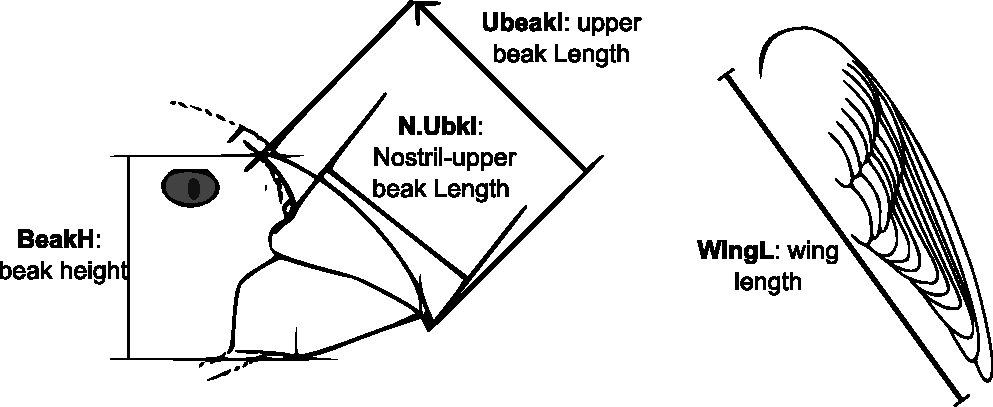
\includegraphics[width = 10cm]{figs/darwinfinch.pdf}
\end{center}

\newpage


%%%%%%%%%%%%%%%%
\section{Description of traits distributions}
%%%%%%%%%%%%%%%%

\subsection{Plot the kernel density of traits}

Plot the distribution of traits values for populations, species, sites and regional scales. First, let try the distribution for all populations of Darwin finches. In R, FALSE and TRUE can be written respectively \texttt{F} and \texttt{T}.

\begin{knitrout}
\definecolor{shadecolor}{rgb}{0.969, 0.969, 0.969}\color{fgcolor}\begin{kframe}
\begin{alltt}
\hlkwd{par}\hlstd{(}\hlkwc{mfrow} \hlstd{=} \hlkwd{c}\hlstd{(}\hlnum{4}\hlstd{,}\hlnum{4}\hlstd{),} \hlkwc{cex} \hlstd{=} \hlnum{0.5}\hlstd{)}
\hlkwd{plotDistri}\hlstd{(traits.finch, sp.finch, ind.plot.finch,}
     \hlkwc{ylim.cex} \hlstd{=} \hlnum{3}\hlstd{,} \hlkwc{plot.ask} \hlstd{= F,} \hlkwc{multipanel} \hlstd{= F,} \hlkwc{leg} \hlstd{= F)}
\end{alltt}


{\ttfamily\noindent\bfseries\color{errorcolor}{\#\# Error: impossible de trouver la fonction "{}plotDistri"{}}}\end{kframe}
\end{knitrout}
The argument \texttt{ylim.cex} define the magnification to be used for range of y axe. To understand the other argument, type \texttt{?plotDistri}.

\newpage

Then we can inverse the second and the third arguments to plot the distribution for all finches species. 

\begin{knitrout}
\definecolor{shadecolor}{rgb}{0.969, 0.969, 0.969}\color{fgcolor}\begin{kframe}
\begin{alltt}
\hlkwd{par}\hlstd{(}\hlkwc{mfrow} \hlstd{=} \hlkwd{c}\hlstd{(}\hlnum{4}\hlstd{,}\hlnum{4}\hlstd{),} \hlkwc{cex} \hlstd{=} \hlnum{0.5}\hlstd{)}
\hlkwd{plotDistri}\hlstd{(traits.finch, ind.plot.finch, sp.finch,}
      \hlkwc{ylim.cex} \hlstd{=} \hlnum{8}\hlstd{,} \hlkwc{plot.ask} \hlstd{= F,} \hlkwc{multipanel} \hlstd{= F,} \hlkwc{leg} \hlstd{= F)}
\end{alltt}


{\ttfamily\noindent\bfseries\color{errorcolor}{\#\# Error: impossible de trouver la fonction "{}plotDistri"{}}}\end{kframe}
\end{knitrout}

Now, see the result for only one trait with the legend (\texttt{leg = TRUE}). \texttt{cex.leg} specify the magnification of legend. 

\begin{knitrout}
\definecolor{shadecolor}{rgb}{0.969, 0.969, 0.969}\color{fgcolor}\begin{kframe}
\begin{alltt}
\hlkwd{par}\hlstd{(}\hlkwc{mfrow} \hlstd{=} \hlkwd{c}\hlstd{(}\hlnum{2}\hlstd{,}\hlnum{3}\hlstd{))}
\hlkwd{plotDistri}\hlstd{(}\hlkwd{as.matrix}\hlstd{(traits.finch[,}\hlnum{1}\hlstd{]), ind.plot.finch, sp.finch,}
     \hlkwc{ylim.cex} \hlstd{=} \hlnum{8}\hlstd{,} \hlkwc{plot.ask} \hlstd{= F,} \hlkwc{multipanel} \hlstd{= F,} \hlkwc{leg} \hlstd{= T,} \hlkwc{cex.leg} \hlstd{=} \hlnum{0.5}\hlstd{)}
\end{alltt}


{\ttfamily\noindent\bfseries\color{errorcolor}{\#\# Error: impossible de trouver la fonction "{}plotDistri"{}}}\end{kframe}
\end{knitrout}

If we want to plot all the sites (regional distribution) or all the species: we can use the following code:
\begin{knitrout}
\definecolor{shadecolor}{rgb}{0.969, 0.969, 0.969}\color{fgcolor}\begin{kframe}
\begin{alltt}
\hlkwd{par}\hlstd{(}\hlkwc{mfrow} \hlstd{=} \hlkwd{c}\hlstd{(}\hlnum{4}\hlstd{,}\hlnum{4}\hlstd{),} \hlkwc{cex} \hlstd{=} \hlnum{0.5}\hlstd{)}
\hlkwd{plotDistri}\hlstd{(traits.finch,} \hlkwd{rep}\hlstd{(}\hlstr{"region"}\hlstd{,} \hlkwc{times} \hlstd{=} \hlkwd{dim}\hlstd{(traits.finch)[}\hlnum{1}\hlstd{]),}
     \hlstd{sp.finch,} \hlkwc{ylim.cex} \hlstd{=} \hlnum{6}\hlstd{,} \hlkwc{plot.ask} \hlstd{= F,} \hlkwc{leg} \hlstd{= F)}
\end{alltt}


{\ttfamily\noindent\bfseries\color{errorcolor}{\#\# Error: impossible de trouver la fonction "{}plotDistri"{}}}\end{kframe}
\end{knitrout}

\begin{knitrout}
\definecolor{shadecolor}{rgb}{0.969, 0.969, 0.969}\color{fgcolor}\begin{kframe}
\begin{alltt}
\hlkwd{plotDistri}\hlstd{(traits.finch,} \hlkwd{rep}\hlstd{(}\hlstr{"toutes_sp"}\hlstd{,} \hlkwc{times} \hlstd{=} \hlkwd{dim}\hlstd{(traits.finch)[}\hlnum{1}\hlstd{]),}
     \hlstd{ind.plot.finch,} \hlkwc{ylim.cex} \hlstd{=} \hlnum{3}\hlstd{,} \hlkwc{plot.ask} \hlstd{= F,} \hlkwc{cex.leg} \hlstd{=} \hlnum{0.5}\hlstd{)}
\end{alltt}


{\ttfamily\noindent\bfseries\color{errorcolor}{\#\# Error: impossible de trouver la fonction "{}plotDistri"{}}}\end{kframe}
\end{knitrout}

Now we can reset the default graphical parameter:
\begin{knitrout}
\definecolor{shadecolor}{rgb}{0.969, 0.969, 0.969}\color{fgcolor}\begin{kframe}
\begin{alltt}
\hlkwd{par}\hlstd{(old.par)}
\end{alltt}
\end{kframe}
\end{knitrout}
\newpage

%%%%%%%%%%%%%%%%
\section{Decomposition of variances}
%%%%%%%%%%%%%%%%

\subsection{Decomposition of within/among species variances using rao diversity}

The Rao function computes $\alpha$, $\beta$ and $\gamma$ -components for taxonomic, functional and/or phylogenetic diversity with:

<<<<<<< HEAD
$$ \gamma = mean (\alpha) + \beta $$
=======
\[ \gamma = mean \alpha + \beta \]



Where: $\gamma$ is the diversity of the regional pool, $\alpha$ is the diversity of the local community and $\beta$ is the turn over between local communities; diversity is estimated using the Rao quadratic entropy indices. Note that this method uses the additive framework of diversity. See the paper of Jost in 2010 (partitioning diversity into independent alpha and beta components) for more details on the differences between additive and multiplicative partitioning of diversity.
>>>>>>> 5f89dfbb4bbfa61805f8e116f94cee418c14cfee


Where: $\gamma$ is the diversity of the regional pool, $\alpha$ is the diversity of the local community and $\beta$ is the turn over between local communities; diversity is estimated using the Rao quadratic entropy indices. Note that this method uses the additive framework of diversity. See the paper of Jost in 2010 (partitioning diversity into independent alpha and beta components) for more details on the differences between additive and multiplicative partitioning of diversity.

\\

\textbf{Reference}: de Bello, F., Lavorel, S., Albert, C.H., Thuiller, W., Grigulis, K., Dolezal, J., Janecek, S. and Leps, J. (2011) Quantifying the relevance of intraspecific trait variability for functional diversity. Methods in Ecology and Evolution, 2, 163-174.


\subsubsection{Multitraits analysis}
First, rao diversity can be calculated on the functional  space (i.e. considering all traits together).

\begin{knitrout}
\definecolor{shadecolor}{rgb}{0.969, 0.969, 0.969}\color{fgcolor}\begin{kframe}
\begin{alltt}
\hlcom{#create individuals community matrix}
\hlstd{comm}\hlkwb{<-}\hlkwd{t}\hlstd{(}\hlkwd{table}\hlstd{(ind.plot.finch,}\hlnum{1}\hlopt{:}\hlkwd{length}\hlstd{(ind.plot.finch)))}
\hlcom{#create species community matrix}
\hlstd{comm.sp}\hlkwb{<-}\hlkwd{table}\hlstd{(sp.finch, ind.plot.finch)}
\hlkwd{class}\hlstd{(comm.sp)}\hlkwb{<-}\hlstr{"matrix"}

\hlstd{traits.finch.sp}\hlkwb{<-}\hlkwd{apply}\hlstd{(} \hlkwd{apply}\hlstd{(traits.finch,} \hlnum{2}\hlstd{, scale ),} \hlnum{2}\hlstd{,}
            \hlkwa{function}\hlstd{(}\hlkwc{x}\hlstd{)} \hlkwd{tapply}\hlstd{(x, sp.finch, mean,} \hlkwc{na.rm} \hlstd{= T))}

\hlstd{mat.dist}\hlkwb{<-}\hlkwd{as.matrix}\hlstd{(}\hlkwd{dist}\hlstd{(traits.finch.sp))}\hlopt{^}\hlnum{2}

\hlstd{res.rao}\hlkwb{<-}\hlkwd{RaoRel}\hlstd{(}\hlkwc{sample} \hlstd{=} \hlkwd{as.matrix}\hlstd{(comm.sp),}
        \hlkwc{dfunc} \hlstd{= mat.dist,} \hlkwc{dphyl} \hlstd{=} \hlkwa{NULL}\hlstd{,}
        \hlkwc{weight} \hlstd{= F,} \hlkwc{Jost} \hlstd{= F,} \hlkwc{structure} \hlstd{=} \hlkwa{NULL}\hlstd{)}

\hlstd{witRao}\hlkwb{<-}\hlstd{res.rao}\hlopt{$}\hlstd{FD}\hlopt{$}\hlstd{Mean_Alpha} \hlcom{#overall within species variance}
\hlstd{betRao}\hlkwb{<-}\hlstd{res.rao}\hlopt{$}\hlstd{FD}\hlopt{$}\hlstd{Beta_add}  \hlcom{#between species variance}
\hlstd{totRao}\hlkwb{<-}\hlstd{res.rao}\hlopt{$}\hlstd{FD}\hlopt{$}\hlstd{Gamma}    \hlcom{#the total variance}

\hlcom{#Check that the total variance is equal}
\hlcom{#to between species + within species variances}
\hlstd{witRao}\hlopt{+}\hlstd{betRao}
\end{alltt}
\begin{verbatim}
## [1] 8.37
\end{verbatim}
\begin{alltt}
\hlstd{totRao}
\end{alltt}
\begin{verbatim}
## [1] 8.37
\end{verbatim}
\end{kframe}
\end{knitrout}

Now let's take the abundance into account to calculate Rao diversity.

\begin{knitrout}
\definecolor{shadecolor}{rgb}{0.969, 0.969, 0.969}\color{fgcolor}\begin{kframe}
\begin{alltt}
\hlstd{res.rao.w}\hlkwb{<-}\hlkwd{RaoRel}\hlstd{(}\hlkwc{sample} \hlstd{=} \hlkwd{as.matrix}\hlstd{(comm.sp),}
         \hlkwc{dfunc} \hlstd{= mat.dist,} \hlkwc{dphyl} \hlstd{=} \hlkwa{NULL}\hlstd{,}
         \hlkwc{weight} \hlstd{= T,} \hlkwc{Jost} \hlstd{= F,} \hlkwc{structure} \hlstd{=} \hlkwa{NULL}\hlstd{)}

\hlstd{witRao.w}\hlkwb{<-}\hlstd{res.rao.w}\hlopt{$}\hlstd{FD}\hlopt{$}\hlstd{Mean_Alpha} \hlcom{#overall within species variance}
\hlstd{betRao.w}\hlkwb{<-}\hlstd{res.rao.w}\hlopt{$}\hlstd{FD}\hlopt{$}\hlstd{Beta_add}  \hlcom{#between species variance}
\hlstd{totRao.w}\hlkwb{<-}\hlstd{res.rao.w}\hlopt{$}\hlstd{FD}\hlopt{$}\hlstd{Gamma}    \hlcom{#the total variance}

\hlstd{witRao.w}
\end{alltt}
\begin{verbatim}
## [1] 7.551
\end{verbatim}
\begin{alltt}
\hlstd{betRao.w}
\end{alltt}
\begin{verbatim}
## [1] 0.3458
\end{verbatim}
\end{kframe}
\end{knitrout}

Plot the results.

\begin{knitrout}
\definecolor{shadecolor}{rgb}{0.969, 0.969, 0.969}\color{fgcolor}\begin{kframe}
\begin{alltt}
\hlkwd{barplot}\hlstd{(}\hlkwd{cbind}\hlstd{(}\hlkwd{c}\hlstd{(witRao.w, betRao.w),} \hlkwd{c}\hlstd{(witRao, betRao)),}
    \hlkwc{names.arg} \hlstd{=} \hlkwd{c}\hlstd{(}\hlstr{"abundance"} \hlstd{,}\hlstr{"presence"}\hlstd{),}
    \hlkwc{legend.text} \hlstd{=} \hlkwd{c}\hlstd{(}\hlstr{"within species"}\hlstd{,} \hlstr{"between species"}\hlstd{),}
    \hlkwc{ylab} \hlstd{=} \hlstr{"Rao"}\hlstd{,} \hlkwc{ylim} \hlstd{=} \hlkwd{c}\hlstd{(}\hlnum{0}\hlstd{,}\hlnum{10}\hlstd{))}
\end{alltt}
\end{kframe}

{\centering 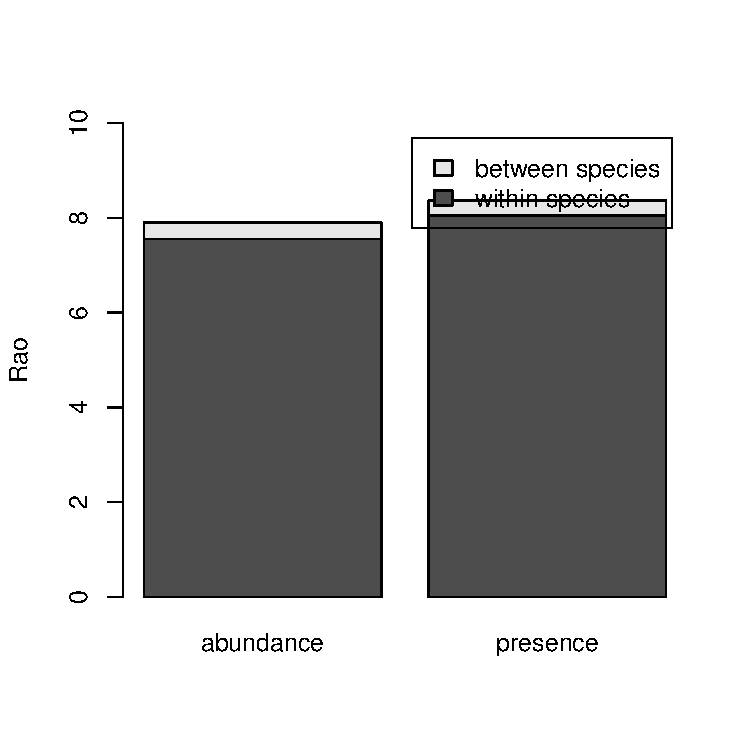
\includegraphics[width=\maxwidth]{figure/unnamed-chunk-18} 

}



\end{knitrout}


\subsubsection{Unitraits analysis}
We can also do this analysis for each trait separately. We need to replace (or exclude) NA values. For this example, we use the package \texttt{mice} to complete the data.

\begin{knitrout}
\definecolor{shadecolor}{rgb}{0.969, 0.969, 0.969}\color{fgcolor}\begin{kframe}
\begin{alltt}
\hlstd{comm}\hlkwb{<-}\hlkwd{t}\hlstd{(}\hlkwd{table}\hlstd{(ind.plot.finch,}\hlnum{1}\hlopt{:}\hlkwd{length}\hlstd{(ind.plot.finch)))}

\hlkwd{require}\hlstd{(mice)}
\hlstd{traits} \hlkwb{=} \hlstd{traits.finch}
\hlstd{mice}\hlkwb{<-}\hlkwd{mice}\hlstd{(traits.finch)}
\hlstd{traits.finch.mice}\hlkwb{<-}\hlkwd{complete}\hlstd{(mice)}
\end{alltt}
\end{kframe}
\end{knitrout}


\begin{knitrout}
\definecolor{shadecolor}{rgb}{0.969, 0.969, 0.969}\color{fgcolor}\begin{kframe}
\begin{alltt}
\hlcom{#Calculate the mean traits value by population using the mice dataset}
\hlstd{traits.finch.mice.sp}\hlkwb{<-}\hlkwd{apply}\hlstd{(}\hlkwd{apply}\hlstd{(traits.finch.mice,} \hlnum{2}\hlstd{, scale ),} \hlnum{2}\hlstd{,}
              \hlkwa{function}\hlstd{(}\hlkwc{x}\hlstd{)} \hlkwd{tapply}\hlstd{(x, sp.finch, mean,} \hlkwc{na.rm} \hlstd{= T))}

\hlstd{trait.rao.w}\hlkwb{<-}\hlkwd{list}\hlstd{()}
\hlstd{witRao.w.bytrait}\hlkwb{<-}\hlkwd{c}\hlstd{()}
\hlstd{betRao.w.bytrait}\hlkwb{<-}\hlkwd{c}\hlstd{()}
\hlkwa{for}\hlstd{(t} \hlkwa{in} \hlnum{1} \hlopt{:} \hlnum{4}\hlstd{)\{}
 \hlstd{trait.rao.w[[t]]}\hlkwb{<-}\hlkwd{RaoRel}\hlstd{(}\hlkwc{sample} \hlstd{=} \hlkwd{as.matrix}\hlstd{(comm.sp),}
              \hlkwc{dfunc} \hlstd{=} \hlkwd{dist}\hlstd{(traits.finch.mice.sp[,t]),}
              \hlkwc{dphyl} \hlstd{=} \hlkwa{NULL}\hlstd{,} \hlkwc{weight} \hlstd{= T,} \hlkwc{Jost} \hlstd{= F,} \hlkwc{structure} \hlstd{=} \hlkwa{NULL}\hlstd{)}
 \hlstd{witRao.w.bytrait}\hlkwb{<-}\hlkwd{c}\hlstd{(witRao.w.bytrait, trait.rao.w[[t]]}\hlopt{$}\hlstd{FD}\hlopt{$}\hlstd{Mean_Alpha)}
 \hlstd{betRao.w.bytrait}\hlkwb{<-}\hlkwd{c}\hlstd{(betRao.w.bytrait, trait.rao.w[[t]]}\hlopt{$}\hlstd{FD}\hlopt{$}\hlstd{Beta_add)}
\hlstd{\}}
\end{alltt}
\end{kframe}
\end{knitrout}

Plot the results by traits.

\begin{knitrout}
\definecolor{shadecolor}{rgb}{0.969, 0.969, 0.969}\color{fgcolor}\begin{kframe}
\begin{alltt}
\hlkwd{barplot}\hlstd{(}\hlkwd{t}\hlstd{(}\hlkwd{cbind}\hlstd{( witRao.w.bytrait, betRao.w.bytrait)),}
    \hlkwc{names.arg} \hlstd{=} \hlkwd{colnames}\hlstd{(traits.finch),}
    \hlkwc{legend.text} \hlstd{=} \hlkwd{c}\hlstd{(}\hlstr{"within species"}\hlstd{,} \hlstr{"between species"}\hlstd{),}
    \hlkwc{ylab} \hlstd{=} \hlstr{"Rao"}\hlstd{,} \hlkwc{ylim} \hlstd{=} \hlkwd{c}\hlstd{(}\hlnum{0}\hlstd{,}\hlnum{1.5}\hlstd{))}
\end{alltt}
\end{kframe}

{\centering 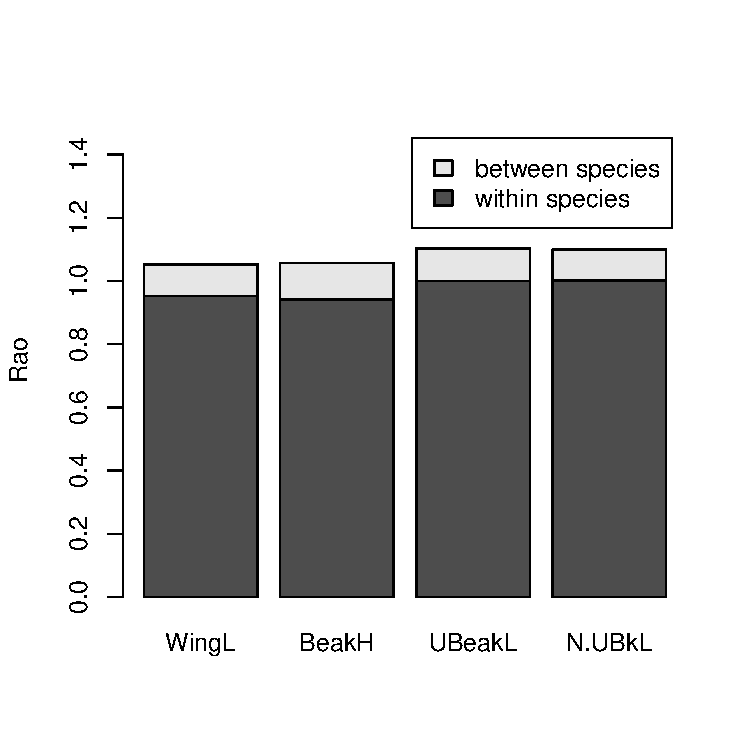
\includegraphics[width=\maxwidth]{figure/unnamed-chunk-21} 

}



\end{knitrout}


\subsection{Decomposition of community trait response to environment into intraspecific trait variability, variability due to species turnover and their covariation.}

\textbf{Reference}: Leps, J., de Bello, F., Smilauer, P. and Dolezal, J. (2011) Community trait response to environment: disentangling species turnover vs intraspecific trait variability effects. Ecography, 34, 856-863.

\begin{knitrout}
\definecolor{shadecolor}{rgb}{0.969, 0.969, 0.969}\color{fgcolor}\begin{kframe}
\begin{alltt}
\hlstd{res.decomp}\hlkwb{<-}\hlkwd{decompCTRE}\hlstd{(}\hlkwc{traits} \hlstd{= traits.finch,} \hlkwc{sp} \hlstd{= sp.finch,}
              \hlkwc{ind.plot} \hlstd{= ind.plot.finch,} \hlkwc{print} \hlstd{=} \hlnum{FALSE}\hlstd{)}
\end{alltt}


{\ttfamily\noindent\bfseries\color{errorcolor}{\#\# Error: impossible de trouver la fonction "{}decompCTRE"{}}}\begin{alltt}
\hlkwd{barplot}\hlstd{(res.decomp)}
\end{alltt}


{\ttfamily\noindent\bfseries\color{errorcolor}{\#\# Error: objet 'res.decomp' introuvable}}\end{kframe}
\end{knitrout}

\begin{knitrout}
\definecolor{shadecolor}{rgb}{0.969, 0.969, 0.969}\color{fgcolor}\begin{kframe}
\begin{alltt}
\hlkwd{par}\hlstd{(}\hlkwc{mfrow} \hlstd{=} \hlkwd{c}\hlstd{(}\hlnum{2}\hlstd{,}\hlnum{2}\hlstd{))}
\hlkwd{barplot}\hlstd{(res.decomp,} \hlkwc{resume} \hlstd{= F)}
\end{alltt}


{\ttfamily\noindent\bfseries\color{errorcolor}{\#\# Error: objet 'res.decomp' introuvable}}\begin{alltt}
\hlkwd{par}\hlstd{(}\hlkwc{mfrow} \hlstd{=} \hlkwd{c}\hlstd{(}\hlnum{1}\hlstd{,}\hlnum{1}\hlstd{))}
\end{alltt}
\end{kframe}
\end{knitrout}

\newpage

\subsection{Decomposition of traits variances using nested factors}

Variance partitioning across nested scales using the decomposition of variance on restricted maximum likelihood (REML) method (lme function).
\\

\textbf{Reference}: Messier, J., McGill, B. and Lechowicz, M. (2010) How do traits vary across ecological scales? A case for trait-based ecology. Ecology Letters, 13, 838-848.

\begin{knitrout}
\definecolor{shadecolor}{rgb}{0.969, 0.969, 0.969}\color{fgcolor}\begin{kframe}
\begin{alltt}
\hlstd{vec}\hlkwb{<-} \hlkwd{seq}\hlstd{(}\hlnum{1}\hlstd{,}\hlkwd{length}\hlstd{(sp.finch)}\hlopt{*}\hlnum{2}\hlstd{,} \hlkwc{by} \hlstd{=} \hlnum{2}\hlstd{)}
\hlstd{genus}\hlkwb{<-}\hlkwd{as.vector}\hlstd{(}\hlkwd{unlist}\hlstd{(}\hlkwd{strsplit}\hlstd{(}\hlkwd{as.vector}\hlstd{(sp.finch),}\hlstr{"_"}\hlstd{))[vec])}
\hlstd{fact}\hlkwb{<-}\hlkwd{cbind}\hlstd{(}\hlkwc{genus} \hlstd{=} \hlkwd{as.factor}\hlstd{(genus),}
      \hlkwc{species} \hlstd{=} \hlkwd{as.factor}\hlstd{(}\hlkwd{as.vector}\hlstd{(sp.finch)),}
      \hlkwc{sites} \hlstd{=} \hlkwd{as.factor}\hlstd{(}\hlkwd{as.vector}\hlstd{(ind.plot.finch)))}

\hlstd{res.partvar.finch}\hlkwb{<-}\hlkwd{partvar}\hlstd{(}\hlkwc{traits} \hlstd{= traits.finch,} \hlkwc{factors} \hlstd{= fact)}

\hlstd{res.partvar.finch}
\end{alltt}
\end{kframe}
\end{knitrout}


\begin{knitrout}
\definecolor{shadecolor}{rgb}{0.969, 0.969, 0.969}\color{fgcolor}\begin{kframe}
\begin{alltt}
\hlkwd{par}\hlstd{(}\hlkwc{mfrow} \hlstd{=} \hlkwd{c}\hlstd{(}\hlnum{2}\hlstd{,}\hlnum{2}\hlstd{),} \hlkwc{mai} \hlstd{=} \hlkwd{c}\hlstd{(}\hlnum{0.2}\hlstd{,}\hlnum{0.2}\hlstd{,}\hlnum{0.2}\hlstd{,}\hlnum{0.2}\hlstd{))} \hlcom{#save graphical parameters}
\hlstd{colors}\hlkwb{<-}\hlkwd{c}\hlstd{(}\hlkwd{rgb}\hlstd{(}\hlnum{102}\hlstd{,}\hlnum{167}\hlstd{,}\hlnum{0}\hlstd{,} \hlkwc{maxColorValue} \hlstd{=} \hlnum{255}\hlstd{),}
     \hlkwd{rgb}\hlstd{(}\hlnum{185}\hlstd{,}\hlnum{210}\hlstd{,}\hlnum{0}\hlstd{,} \hlkwc{maxColorValue} \hlstd{=} \hlnum{255}\hlstd{),}
     \hlkwd{rgb}\hlstd{(}\hlnum{98}\hlstd{,}\hlnum{174}\hlstd{,}\hlnum{255}\hlstd{,} \hlkwc{maxColorValue} \hlstd{=} \hlnum{255}\hlstd{),}
     \hlkwd{rgb}\hlstd{(}\hlnum{158}\hlstd{,}\hlnum{30}\hlstd{,}\hlnum{240}\hlstd{,} \hlkwc{maxColorValue} \hlstd{=} \hlnum{255}\hlstd{))}

\hlkwd{piePartvar}\hlstd{(res.partvar.finch,} \hlkwc{col} \hlstd{= colors)}
\end{alltt}


{\ttfamily\noindent\bfseries\color{errorcolor}{\#\# Error: impossible de trouver la fonction "{}piePartvar"{}}}\begin{alltt}
\hlkwd{par}\hlstd{(old.par)} \hlcom{#reset old graphical parameters}
\end{alltt}
\end{kframe}
\end{knitrout}

\begin{knitrout}
\definecolor{shadecolor}{rgb}{0.969, 0.969, 0.969}\color{fgcolor}\begin{kframe}
\begin{alltt}
\hlkwd{barPartvar}\hlstd{(res.partvar.finch,} \hlkwc{col} \hlstd{= colors,} \hlkwc{leg} \hlstd{=} \hlnum{TRUE}\hlstd{)}
\end{alltt}
<<<<<<< HEAD
\end{kframe}

{\centering 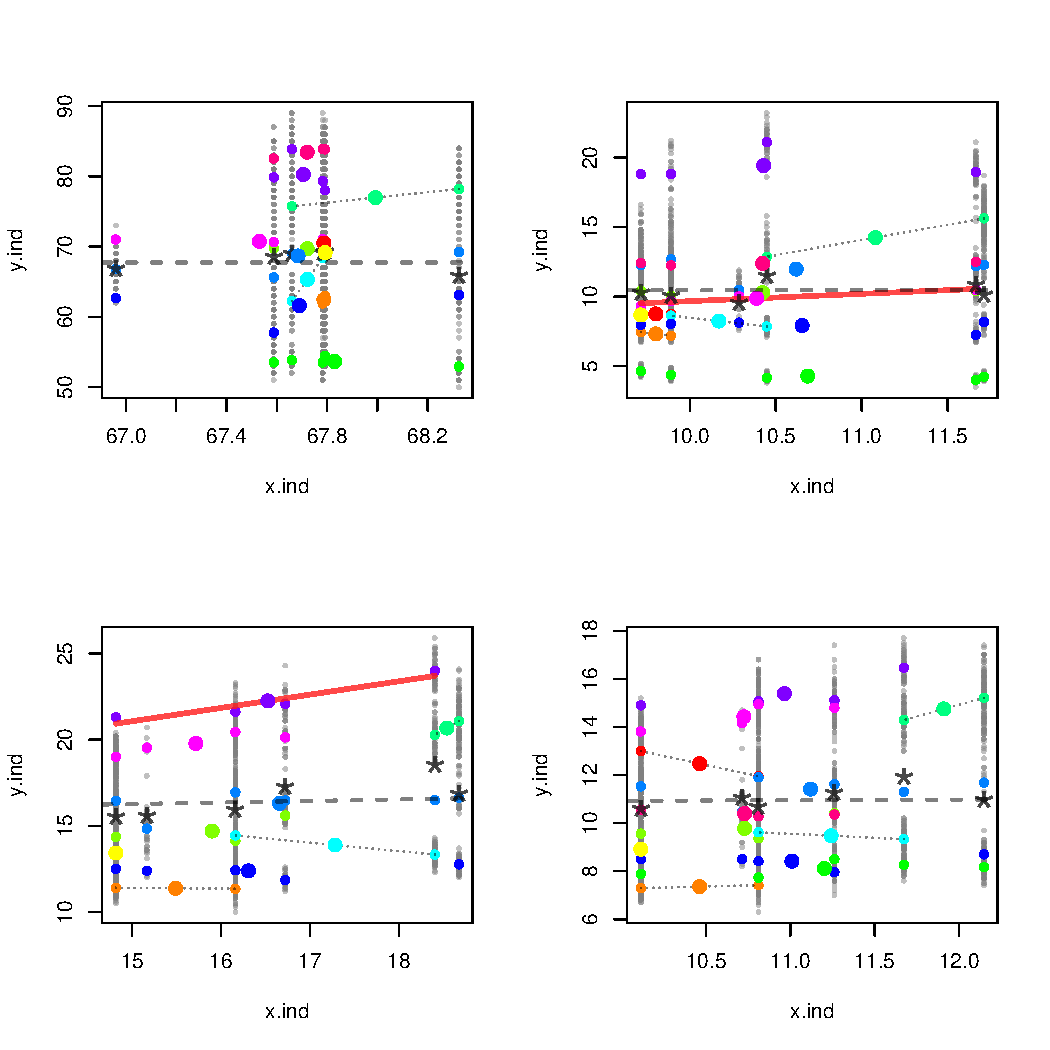
\includegraphics[width=\maxwidth]{figure/unnamed-chunk-26} 

}

=======
>>>>>>> 5f89dfbb4bbfa61805f8e116f94cee418c14cfee


{\ttfamily\noindent\bfseries\color{errorcolor}{\#\# Error: impossible de trouver la fonction "{}barPartvar"{}}}\end{kframe}
\end{knitrout}


\newpage

\subsection{Plot the relation between populational trait means and sites traits means.}

For an example of utilisation see: Cornwell, W.K. and Ackerly, D.D., 2009. Community assembly and shifts in plant trait distributions across an environmental gradient in coastal California. Ecological Monographs, 79, 109-126.

\begin{knitrout}
\definecolor{shadecolor}{rgb}{0.969, 0.969, 0.969}\color{fgcolor}\begin{kframe}
\begin{alltt}
\hlkwd{plotSpPop}\hlstd{(traits.finch, ind.plot.finch, sp.finch,} \hlkwc{silent} \hlstd{=} \hlnum{TRUE}\hlstd{)}
\end{alltt}


{\ttfamily\noindent\bfseries\color{errorcolor}{\#\# Error: impossible de trouver la fonction "{}plotSpPop"{}}}\end{kframe}
\end{knitrout}

If we change the value of two arguments we can see some significant relationships. Here let's try a more permissive threshold: alpha = 10\% instead of 5\% (\texttt{p.val}) and define a lower minimum of values to represent significance  fixed to 3 instead of 10 by default (\texttt{min.ind.signif}). 

\newpage

\begin{knitrout}
\definecolor{shadecolor}{rgb}{0.969, 0.969, 0.969}\color{fgcolor}\begin{kframe}
\begin{alltt}
\hlkwd{plotSpPop}\hlstd{(traits.finch, ind.plot.finch, sp.finch,}
      \hlkwc{p.val} \hlstd{=} \hlnum{0.1}\hlstd{,} \hlkwc{min.ind.signif} \hlstd{=} \hlnum{3}\hlstd{,} \hlkwc{silent} \hlstd{=} \hlnum{TRUE}\hlstd{)}
\end{alltt}


{\ttfamily\noindent\bfseries\color{errorcolor}{\#\# Error: impossible de trouver la fonction "{}plotSpPop"{}}}\end{kframe}
\end{knitrout}

\newpage

For a more simple figure, add the option resume = TRUE. 
\begin{knitrout}
\definecolor{shadecolor}{rgb}{0.969, 0.969, 0.969}\color{fgcolor}\begin{kframe}
\begin{alltt}
\hlkwd{plotSpPop}\hlstd{(traits.finch, ind.plot.finch, sp.finch,}
      \hlkwc{silent} \hlstd{=} \hlnum{TRUE}\hlstd{,} \hlkwc{resume} \hlstd{=} \hlnum{TRUE}\hlstd{,} \hlkwc{col.pop} \hlstd{=} \hlstr{"grey"}\hlstd{)}
\end{alltt}


{\ttfamily\noindent\bfseries\color{errorcolor}{\#\# Error: impossible de trouver la fonction "{}plotSpPop"{}}}\end{kframe}
\end{knitrout}

If you are fed up with colors, try this:
\begin{knitrout}
\definecolor{shadecolor}{rgb}{0.969, 0.969, 0.969}\color{fgcolor}\begin{kframe}
\begin{alltt}
\hlkwd{plotSpPop}\hlstd{(traits.finch, ind.plot.finch, sp.finch,}
      \hlkwc{silent} \hlstd{=} \hlnum{TRUE}\hlstd{,} \hlkwc{resume} \hlstd{=} \hlnum{TRUE}\hlstd{,} \hlkwc{col.pop} \hlstd{=} \hlstr{"grey"}\hlstd{,} \hlkwc{col.sp} \hlstd{=} \hlstr{"black"}\hlstd{)}
\end{alltt}


{\ttfamily\noindent\bfseries\color{errorcolor}{\#\# Error: impossible de trouver la fonction "{}plotSpPop"{}}}\end{kframe}
\end{knitrout}

Again if we change the value of the threshold (\texttt{p.val} = 0.1 and \texttt{min.ind.signif} = 3) we can see some significant relationships.

\begin{knitrout}
\definecolor{shadecolor}{rgb}{0.969, 0.969, 0.969}\color{fgcolor}\begin{kframe}
\begin{alltt}
\hlkwd{plotSpPop}\hlstd{(traits.finch, ind.plot.finch, sp.finch,}
      \hlkwc{silent} \hlstd{=} \hlnum{TRUE}\hlstd{,} \hlkwc{resume} \hlstd{=} \hlnum{TRUE}\hlstd{,} \hlkwc{col.pop} \hlstd{=} \hlstr{"grey"}\hlstd{,} \hlkwc{col.sp} \hlstd{=} \hlstr{"black"}\hlstd{,}
      \hlkwc{p.val} \hlstd{=} \hlnum{0.1}\hlstd{,} \hlkwc{min.ind.signif} \hlstd{=} \hlnum{3}\hlstd{)}
\end{alltt}


{\ttfamily\noindent\bfseries\color{errorcolor}{\#\# Error: impossible de trouver la fonction "{}plotSpPop"{}}}\end{kframe}
\end{knitrout}


\newpage

%%%%%%%%%%%%%%%%
\section{Test of community assembly}
%%%%%%%%%%%%%%%%

\subsection{Ratio of variances: T-statistics}

The function \texttt{Tstat} computes observed T-statistics (T for Traits; Violle et al (2012)) as three ratios of variance, namely $T_{IP/IC}$, $T_{IC/IR}$ and $T_{PC/PR}$. This function can also return the distribution of these three statistics under the three associated null models (respectively \textbf{local}, \textbf{regional.ind} and \textbf{regional.pop}).
\\

\textbf{Reference}: Violle, C., Enquist, B.J., McGill, B.J., Jiang, L., Albert, C., Hulshof, C., Jung, V. and Messier, J. (2012) The return of the variance: intraspecific variability in community ecology. Trends in Ecology and Evolution, 27, 244-252.

\begin{knitrout}
\definecolor{shadecolor}{rgb}{0.969, 0.969, 0.969}\color{fgcolor}\begin{kframe}
\begin{alltt}
\hlstd{res.finch}\hlkwb{<-}\hlkwd{Tstats}\hlstd{(traits.finch,} \hlkwc{ind.plot} \hlstd{= ind.plot.finch,} \hlkwc{sp} \hlstd{= sp.finch,}
         \hlkwc{nperm} \hlstd{=} \hlnum{9}\hlstd{,} \hlkwc{print} \hlstd{=} \hlnum{FALSE}\hlstd{)}
\end{alltt}


{\ttfamily\noindent\bfseries\color{errorcolor}{\#\# Error: argument inutilisé (ind.plot = ind.plot.finch)}}\begin{alltt}
\hlstd{res.finch}
\end{alltt}
<<<<<<< HEAD
\begin{verbatim}
## 	##################
## 	# T-statistiques #
## 	##################
## class: Tstats
## $call: Tstats(traits = traits.finch, ind.plot = ind.plot.finch, sp = sp.finch, 
##     nperm = 9, printprogress = FALSE)
## 
## ###############
## $Tstats: list of observed and null T-statistics
## 
## Observed values
## 	$T_IP.IC: ratio of within-population variance to total within-community variance
## 	$T_IC.IR: community-wide variance relative to the total variance in the regional pool
## 	$T_PC.PR: inter-community variance relative to the total variance in the regional pool
## 
## Null values, number of permutation: 9
## 	$T_IP.IC_nm: distribution of T_IP.IC value under the null model local
## 	$T_IC.IR_nm: distribution of T_IC.IR value under the null model regional.ind 
## 	$T_PC.PR_nm: distribution of T_PC.PR value under the null model regional.pop
## 
## ###############
## $variances: list of observed and null variances
## 
## ###############
## data used
##   data      class      dim   
## 1 $traits   data.frame 2513,4
## 2 $ind.plot factor     2513  
## 3 $sp       factor     2513  
##   content                                             
## 1 traits data                                         
## 2 name of the plot in which the individual is         
## 3 groups (e.g. species) which the individual belong to
## 
## ###############
## others
## 	$namestraits: 4 traits
## [1] "WingL"  "BeakH"  "UBeakL" "N.UBkL"
## 
## 	$sites_richness:
## 	ind.plot
##     DMaj    EspHd FlorChrl  GnovTwr MrchBndl SCruInde 
##       50      267      981      258      270      687
\end{verbatim}
\end{kframe}
=======


{\ttfamily\noindent\bfseries\color{errorcolor}{\#\# Error: objet 'res.finch' introuvable}}\end{kframe}
>>>>>>> 5f89dfbb4bbfa61805f8e116f94cee418c14cfee
\end{knitrout}


\subsubsection{S3 methods for class Tstats}
Tstats class is associated to S3 methods plot, barplot, print and summary. We have already used the print function in the above script line. Now, how to plot the result of the function \texttt{Tstats}?

We can represent observed values thanks to the \texttt{barplot} function.
\begin{knitrout}
\definecolor{shadecolor}{rgb}{0.969, 0.969, 0.969}\color{fgcolor}\begin{kframe}
\begin{alltt}
\hlkwd{barplot}\hlstd{(res.finch,} \hlkwc{ylim} \hlstd{=} \hlkwd{c}\hlstd{(}\hlnum{0}\hlstd{,}\hlnum{3.5}\hlstd{))}
\end{alltt}


{\ttfamily\noindent\bfseries\color{errorcolor}{\#\# Error: objet 'res.finch' introuvable}}\end{kframe}
\end{knitrout}

One can be more interested in the significance  and the effect size available thanks to null model. In that case, the standardized effect size can be easily plot. Note that the function \texttt{ses} can be use directly to calculate standardized effect size without plotting. The Standardized Effect Size (ses) is define as : 

\begin{center}
$$ SES = (I_{obs} – I{_sim}) / \delta_{sim} $$
\end{center}


<<<<<<< HEAD
where $I_{obs}$ is the observed value, $I_{sim}$ the mean of values calculated from the null model and $\delta_{sim}$ the standard deviation of these simulated values.
=======
where $I_obs$ is the observed value, $I_sim$ the mean of values calculated from the null model and $\delta_{sim}$ the standard deviation of these simulated values.
>>>>>>> 5f89dfbb4bbfa61805f8e116f94cee418c14cfee


where $I_obs$ is the observed value, $I_sim$ the mean of values calculated from the null model and $\delta_{sim}$ the standard deviation of these simulated values.


\begin{knitrout}
\definecolor{shadecolor}{rgb}{0.969, 0.969, 0.969}\color{fgcolor}\begin{kframe}
\begin{alltt}
\hlkwd{plot}\hlstd{(res.finch)}
\end{alltt}


{\ttfamily\noindent\bfseries\color{errorcolor}{\#\# Error: objet 'res.finch' introuvable}}\end{kframe}
\end{knitrout}

There is multiple kind of representation avaible.
\begin{knitrout}
\definecolor{shadecolor}{rgb}{0.969, 0.969, 0.969}\color{fgcolor}\begin{kframe}
\begin{alltt}
\hlkwd{plot}\hlstd{(res.finch,} \hlkwc{type} \hlstd{=} \hlstr{"simple"}\hlstd{)}
\end{alltt}


{\ttfamily\noindent\bfseries\color{errorcolor}{\#\# Error: objet 'res.finch' introuvable}}\begin{alltt}
\hlkwd{plot}\hlstd{(res.finch,} \hlkwc{type} \hlstd{=} \hlstr{"simple_range"}\hlstd{)}
\end{alltt}


{\ttfamily\noindent\bfseries\color{errorcolor}{\#\# Error: objet 'res.finch' introuvable}}\begin{alltt}
\hlkwd{plot}\hlstd{(res.finch,} \hlkwc{type} \hlstd{=} \hlstr{"barplot"}\hlstd{)}
\end{alltt}


{\ttfamily\noindent\bfseries\color{errorcolor}{\#\# Error: objet 'res.finch' introuvable}}\end{kframe}
\end{knitrout}

If you want to specifically look at traits or sites statistics, use the argument \texttt{type = "bytraits"} or \texttt{"bysites"}.
\begin{knitrout}
\definecolor{shadecolor}{rgb}{0.969, 0.969, 0.969}\color{fgcolor}\begin{kframe}
\begin{alltt}
\hlkwd{par}\hlstd{(}\hlkwc{mfrow}\hlstd{=}\hlkwd{c}\hlstd{(}\hlnum{2}\hlstd{,}\hlnum{2}\hlstd{))}

\hlkwd{plot}\hlstd{(res.finch,} \hlkwc{type} \hlstd{=} \hlstr{"bytraits"}\hlstd{)}
\end{alltt}
<<<<<<< HEAD
\end{kframe}

{\centering 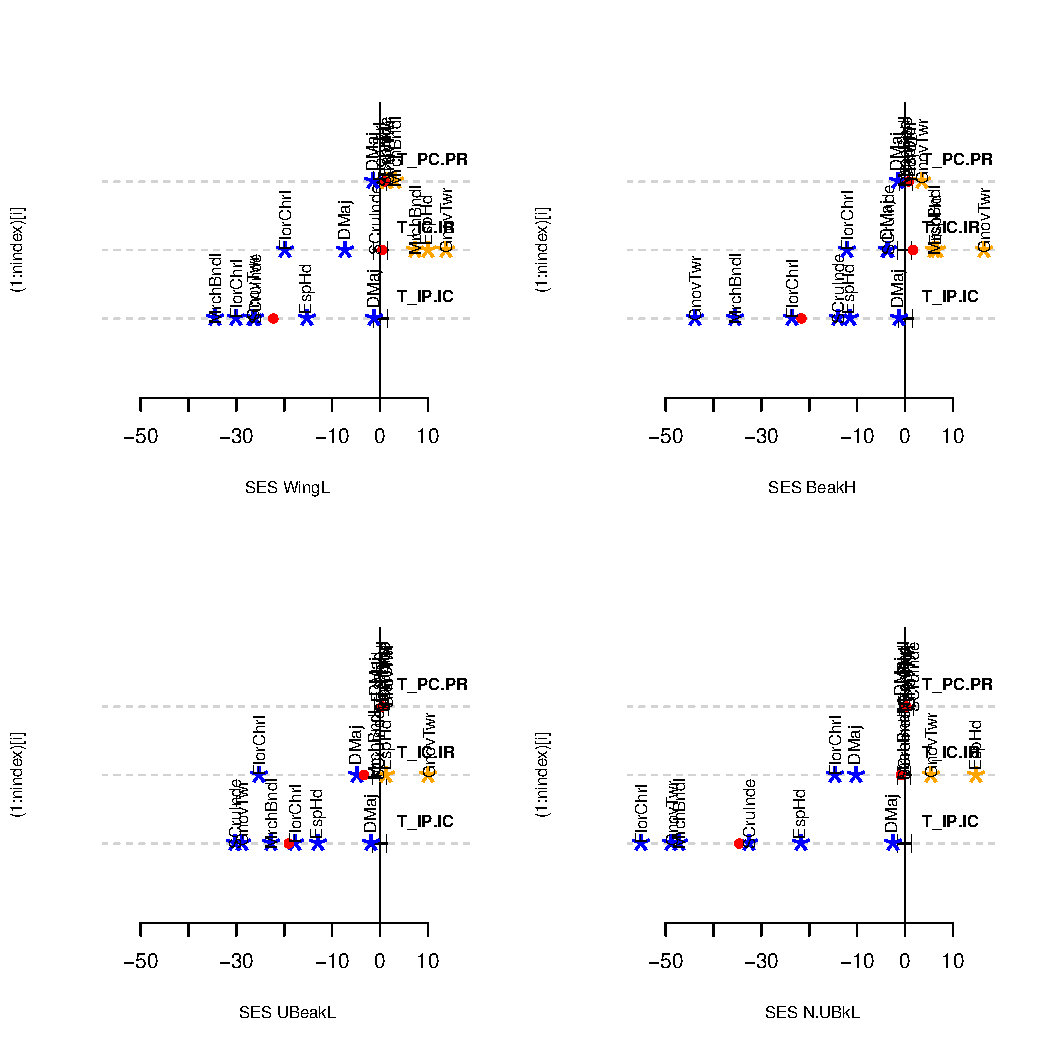
\includegraphics[width=\maxwidth]{figure/unnamed-chunk-361} 

}


\begin{kframe}\begin{alltt}
\hlkwd{plot}\hlstd{(res.finch,} \hlkwc{type} \hlstd{=} \hlstr{"bysites"}\hlstd{)}
\end{alltt}
\end{kframe}

{\centering 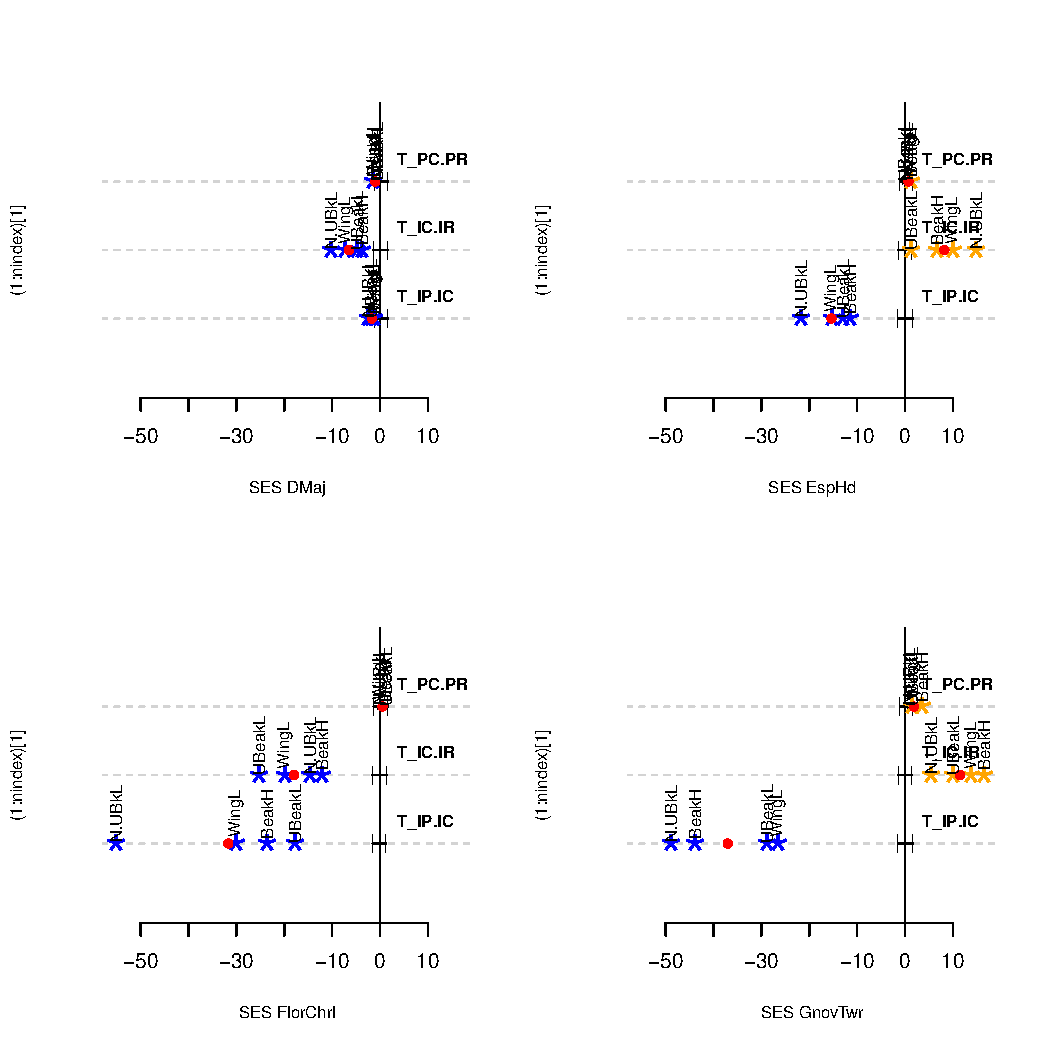
\includegraphics[width=\maxwidth]{figure/unnamed-chunk-362} 

}




{\centering 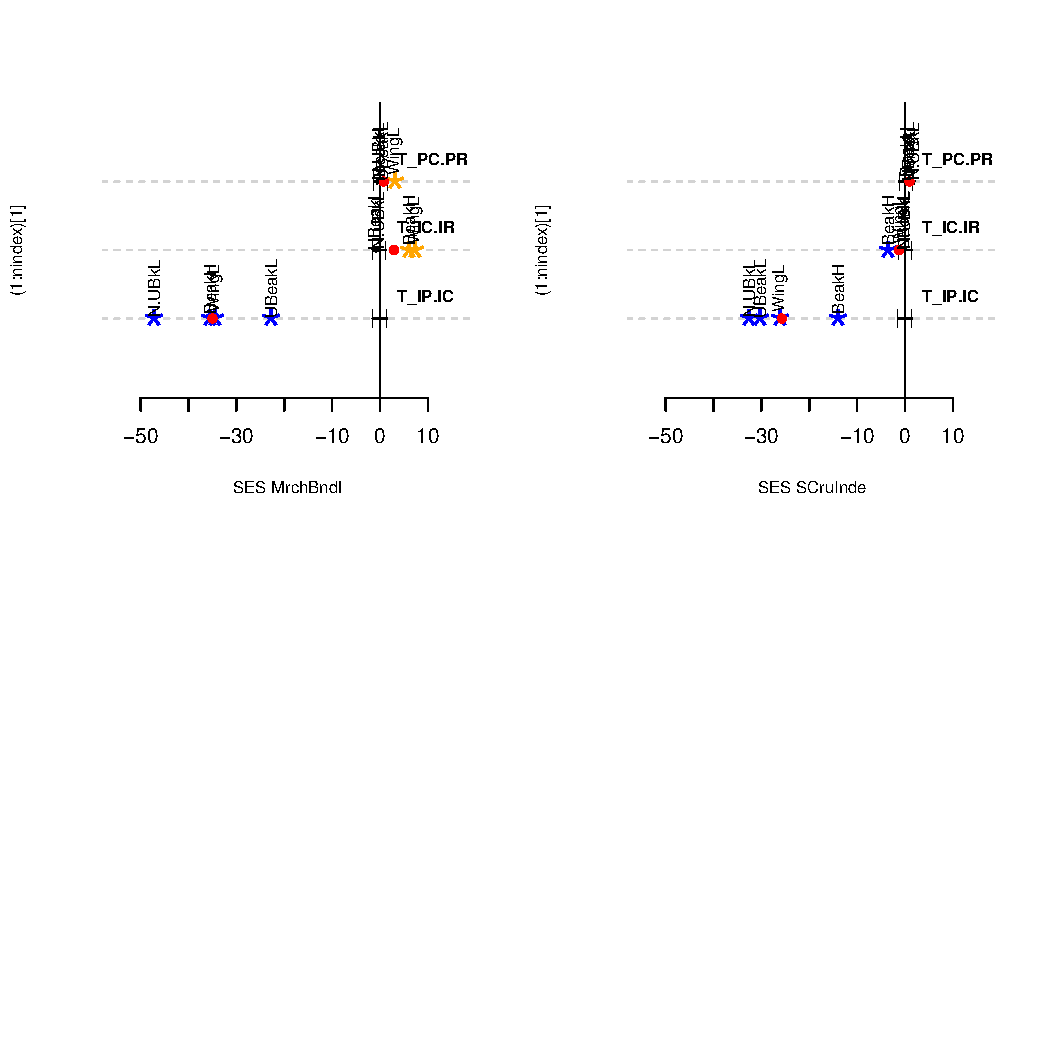
\includegraphics[width=\maxwidth]{figure/unnamed-chunk-363} 

}
=======


{\ttfamily\noindent\bfseries\color{errorcolor}{\#\# Error: objet 'res.finch' introuvable}}\begin{alltt}
\hlkwd{plot}\hlstd{(res.finch,} \hlkwc{type} \hlstd{=} \hlstr{"bysites"}\hlstd{)}
\end{alltt}

>>>>>>> 5f89dfbb4bbfa61805f8e116f94cee418c14cfee

{\ttfamily\noindent\bfseries\color{errorcolor}{\#\# Error: objet 'res.finch' introuvable}}\begin{alltt}
\hlkwd{par}\hlstd{(old.par)} \hlcom{# reset default graphical parameters}
\end{alltt}
\end{kframe}
\end{knitrout}

\newpage

\begin{knitrout}
\definecolor{shadecolor}{rgb}{0.969, 0.969, 0.969}\color{fgcolor}\begin{kframe}
\begin{alltt}
\hlkwd{summary}\hlstd{(res.finch)} \hlcom{#S3 summary method for class Tstats}
\end{alltt}


{\ttfamily\noindent\bfseries\color{errorcolor}{\#\# Error: objet 'res.finch' introuvable}}\end{kframe}
\end{knitrout}


\begin{knitrout}
\definecolor{shadecolor}{rgb}{0.969, 0.969, 0.969}\color{fgcolor}\begin{kframe}
\begin{alltt}
\hlkwd{attributes}\hlstd{(}\hlkwd{sum_Tstats}\hlstd{(res.finch))} \hlcom{#Another mean to summarize Tstatistics}
\end{alltt}


{\ttfamily\noindent\bfseries\color{errorcolor}{\#\# Error: impossible de trouver la fonction "{}sum\_Tstats"{}}}\begin{alltt}
\hlkwd{head}\hlstd{(}\hlkwd{sum_Tstats}\hlstd{(res.finch)}\hlopt{$}\hlstd{p.value,} \hlnum{10}\hlstd{)}
\end{alltt}


{\ttfamily\noindent\bfseries\color{errorcolor}{\#\# Error: impossible de trouver la fonction "{}sum\_Tstats"{}}}\end{kframe}
\end{knitrout}

\newpage

\subsubsection{Plot T-statistics correlations}

We can also see T-statistics correlations and theirs correlation with others variables (e.g. a gradient variable, or the species richness).

\begin{knitrout}
\definecolor{shadecolor}{rgb}{0.969, 0.969, 0.969}\color{fgcolor}\begin{kframe}
\begin{alltt}
\hlkwd{par}\hlstd{(}\hlkwc{mfrow} \hlstd{=} \hlkwd{c}\hlstd{(}\hlnum{2}\hlstd{,}\hlnum{3}\hlstd{))}
\hlkwd{plotCorTstats}\hlstd{(res.finch,} \hlkwc{plot.ask} \hlstd{=} \hlnum{FALSE}\hlstd{,} \hlkwc{multipanel} \hlstd{= F)}
\end{alltt}


{\ttfamily\noindent\bfseries\color{errorcolor}{\#\# Error: impossible de trouver la fonction "{}plotCorTstats"{}}}\end{kframe}
\end{knitrout}

Here we plot T-statistics (in the standardized effect size SES form) in function of species richness by sites.

\begin{knitrout}
\definecolor{shadecolor}{rgb}{0.969, 0.969, 0.969}\color{fgcolor}\begin{kframe}
\begin{alltt}
\hlkwd{par}\hlstd{(}\hlkwc{mfrow} \hlstd{=} \hlkwd{c}\hlstd{(}\hlnum{2}\hlstd{,}\hlnum{2}\hlstd{))}
\hlstd{species.richness}\hlkwb{<-}\hlkwd{table}\hlstd{(ind.plot.finch)}
\hlkwd{plotSESvar}\hlstd{(}\hlkwd{as.listofindex}\hlstd{(}\hlkwd{list}\hlstd{(res.finch)), species.richness,}
       \hlkwc{multipanel} \hlstd{= F)}
\end{alltt}


{\ttfamily\noindent\bfseries\color{errorcolor}{\#\# Error: impossible de trouver la fonction "{}plotSESvar"{}}}\end{kframe}
\end{knitrout}

Same plot with \texttt{resume = TRUE}.

\begin{knitrout}
\definecolor{shadecolor}{rgb}{0.969, 0.969, 0.969}\color{fgcolor}\begin{kframe}
\begin{alltt}
\hlkwd{par}\hlstd{(}\hlkwc{mfrow} \hlstd{=} \hlkwd{c}\hlstd{(}\hlnum{2}\hlstd{,}\hlnum{2}\hlstd{))}
\hlkwd{plotSESvar}\hlstd{(}\hlkwd{as.listofindex}\hlstd{(}\hlkwd{list}\hlstd{(res.finch)), species.richness,}
       \hlkwc{resume} \hlstd{= T,} \hlkwc{multipanel} \hlstd{= F)}
\end{alltt}


{\ttfamily\noindent\bfseries\color{errorcolor}{\#\# Error: impossible de trouver la fonction "{}plotSESvar"{}}}\begin{alltt}
\hlkwd{par}\hlstd{(}\hlkwc{mfrow} \hlstd{=} \hlkwd{c}\hlstd{(}\hlnum{1}\hlstd{,}\hlnum{1}\hlstd{))}
\end{alltt}
\end{kframe}
\end{knitrout}


\newpage
\subsection{Others univariates or multivariates metrics: function \texttt{ComIndex} and \texttt{ComIndexMulti}}

The function \texttt{ComIndex} allow choosing your own function (like mean, range, variance, ...) to calculate customize metrics. Here \texttt{CVNND} refers to the Coefficient of Variation of the Nearest Neighborhood Distance. \texttt{ComIndexMulti} do the same things for multivariate metrics. 

\begin{knitrout}
\definecolor{shadecolor}{rgb}{0.969, 0.969, 0.969}\color{fgcolor}\begin{kframe}
\begin{alltt}
\hlcom{#Define the function s to calculate}
\hlstd{funct}\hlkwb{<-}\hlkwd{c}\hlstd{(}\hlstr{"mean(x, na.rm = T)"}\hlstd{,} \hlstr{"kurtosis(x, na.rm = T)"}\hlstd{,}
     \hlstr{"max(x, na.rm = T) - min(x, na.rm = T)"}\hlstd{,} \hlstr{"CVNND(x)"} \hlstd{)}

\hlcom{#Test against the null model regional.ind}
\hlstd{res.finch.sp_regional.ind}\hlkwb{<-}\hlkwd{ComIndex}\hlstd{(}\hlkwc{traits} \hlstd{= traits.finch,} \hlkwc{index} \hlstd{= funct,} \hlkwc{sp} \hlstd{= sp.finch,}
                           \hlkwc{nullmodels} \hlstd{=} \hlstr{"regional.ind"}\hlstd{,} \hlkwc{ind.plot} \hlstd{= ind.plot.finch,}
                            \hlkwc{nperm} \hlstd{=} \hlnum{9}\hlstd{,} \hlkwc{print} \hlstd{=} \hlnum{FALSE}\hlstd{)}
\end{alltt}


{\ttfamily\noindent\bfseries\color{errorcolor}{\#\# Error: impossible de trouver la fonction "{}ComIndex"{}}}\begin{alltt}
\hlcom{#Test against the null model regional.pop}
\hlcom{#Individuals values are transformed in populational values}
\hlstd{res.finch.sp_regional.pop}\hlkwb{<-}\hlkwd{ComIndex}\hlstd{(}\hlkwc{traits} \hlstd{= traits.finch,} \hlkwc{index} \hlstd{= funct,} \hlkwc{sp} \hlstd{= sp.finch,}
               \hlkwc{nullmodels} \hlstd{=} \hlstr{"regional.pop"}\hlstd{,} \hlkwc{ind.plot} \hlstd{= ind.plot.finch,}
               \hlkwc{nperm} \hlstd{=} \hlnum{9}\hlstd{,} \hlkwc{print} \hlstd{=} \hlnum{FALSE}\hlstd{)}
\end{alltt}


{\ttfamily\noindent\bfseries\color{errorcolor}{\#\# Error: impossible de trouver la fonction "{}ComIndex"{}}}\end{kframe}
\end{knitrout}

These two functions allows to calculate  index by sites for example using \code{"tapply(x, sites, mean)"}.

\begin{knitrout}
\definecolor{shadecolor}{rgb}{0.969, 0.969, 0.969}\color{fgcolor}\begin{kframe}
\begin{alltt}
\hlstd{funct.1}\hlkwb{<-}\hlkwd{c}\hlstd{(}\hlstr{"tapply(x, ind.plot.finch, function(x) mean(x, na.rm = T))"}\hlstd{,}
     \hlstr{"tapply(x, ind.plot.finch, function(x) kurtosis(x, na.rm = T))"}\hlstd{,}
     \hlstr{"tapply(x, ind.plot.finch, function(x) max(x, na.rm = T)-min(x, na.rm = T))"}\hlstd{,}
     \hlstr{"tapply(x, ind.plot.finch, function(x) CVNND(x))"} \hlstd{)}

\hlcom{#The function IndexByGroups permit to easily obtain the above lines }
\hlkwd{IndexByGroups}\hlstd{(funct,} \hlstr{"ind.plot.finch"}\hlstd{)}
\end{alltt}
<<<<<<< HEAD
\begin{verbatim}
## [1] "tapply(x, ind.plot.finch, function(x) mean(x, na.rm = T))"                   
## [2] "tapply(x, ind.plot.finch, function(x) kurtosis(x, na.rm = T))"               
## [3] "tapply(x, ind.plot.finch, function(x) max(x, na.rm = T) - min(x, na.rm = T))"
## [4] "tapply(x, ind.plot.finch, function(x) CVNND(x))"
\end{verbatim}
\begin{alltt}
=======


{\ttfamily\noindent\bfseries\color{errorcolor}{\#\# Error: impossible de trouver la fonction "{}IndexByGroups"{}}}\begin{alltt}
>>>>>>> 5f89dfbb4bbfa61805f8e116f94cee418c14cfee
\hlcom{##Null model local is trivial for these functions}
\hlcom{##because randomization is within community only}

\hlstd{res.finch.ind_loc}\hlkwb{<-}\hlkwd{ComIndex}\hlstd{(}\hlkwc{traits} \hlstd{= traits.finch,} \hlkwc{index} \hlstd{= funct.1,} \hlkwc{sp} \hlstd{= sp.finch,}
               \hlkwc{nullmodels} \hlstd{=} \hlstr{"local"}\hlstd{,} \hlkwc{ind.plot} \hlstd{= ind.plot.finch,}
               \hlkwc{nperm} \hlstd{=} \hlnum{9}\hlstd{,} \hlkwc{print} \hlstd{=} \hlnum{FALSE}\hlstd{)}
<<<<<<< HEAD
=======
\end{alltt}


{\ttfamily\noindent\bfseries\color{errorcolor}{\#\# Error: impossible de trouver la fonction "{}ComIndex"{}}}\begin{alltt}
>>>>>>> 5f89dfbb4bbfa61805f8e116f94cee418c14cfee
\hlstd{res.finch.ind_reg}\hlkwb{<-}\hlkwd{ComIndex}\hlstd{(}\hlkwc{traits} \hlstd{= traits.finch,} \hlkwc{index} \hlstd{= funct.1,} \hlkwc{sp} \hlstd{= sp.finch,}
               \hlkwc{nullmodels} \hlstd{=} \hlstr{"regional.ind"}\hlstd{,} \hlkwc{ind.plot} \hlstd{= ind.plot.finch,}
               \hlkwc{nperm} \hlstd{=} \hlnum{9}\hlstd{,} \hlkwc{print} \hlstd{=} \hlnum{FALSE}\hlstd{)}
\end{alltt}


{\ttfamily\noindent\bfseries\color{errorcolor}{\#\# Error: impossible de trouver la fonction "{}ComIndex"{}}}\end{kframe}
\end{knitrout}


We can calculate index with or without intraspecific variance.

\begin{knitrout}
\definecolor{shadecolor}{rgb}{0.969, 0.969, 0.969}\color{fgcolor}\begin{kframe}
\begin{alltt}
\hlcom{#calculate  of means by population (name_sp_site is a name of a population) }
\hlcom{#determine the site for each population (sites_bypop)}

\hlstd{name_sp_sites} \hlkwb{=} \hlkwd{paste}\hlstd{(sp.finch, ind.plot.finch,} \hlkwc{sep} \hlstd{=} \hlstr{"_"}\hlstd{)}
\hlstd{traits.by.pop}\hlkwb{<-}\hlkwd{apply}\hlstd{(traits.finch,} \hlnum{2} \hlstd{,}
           \hlkwa{function} \hlstd{(}\hlkwc{x}\hlstd{)} \hlkwd{tapply}\hlstd{(x, name_sp_sites, mean ,} \hlkwc{na.rm} \hlstd{= T))}

\hlstd{sites_bypop}\hlkwb{<-}\hlkwd{lapply}\hlstd{(}\hlkwd{strsplit}\hlstd{(}\hlkwd{paste}\hlstd{(}\hlkwd{rownames}\hlstd{(traits.by.pop),} \hlkwc{sep} \hlstd{=} \hlstr{"_"}\hlstd{),} \hlkwc{split} \hlstd{=} \hlstr{"_"}\hlstd{),}
          \hlkwa{function}\hlstd{(}\hlkwc{x}\hlstd{) x[}\hlnum{3}\hlstd{])}

\hlstd{fact}\hlkwb{<-}\hlkwd{unlist}\hlstd{(sites_bypop)}

\hlstd{funct.2}\hlkwb{<-}\hlkwd{c}\hlstd{(}\hlstr{"tapply(x, fact, function(x) mean(x, na.rm = T))"}\hlstd{,}
          \hlstr{"tapply(x, fact, function(x) kurtosis(x, na.rm = T))"}\hlstd{,}
          \hlstr{"tapply(x, fact, function(x) max(x, na.rm = T)-min(x, na.rm = T))"}\hlstd{,}
          \hlstr{"tapply(x, fact, function(x) CVNND(x))"}\hlstd{)}
\end{alltt}
\end{kframe}
\end{knitrout}

Now calculate index with or without intraspecific variance thanks to function \texttt{ComIndex}.
\begin{knitrout}
\definecolor{shadecolor}{rgb}{0.969, 0.969, 0.969}\color{fgcolor}\begin{kframe}
\begin{alltt}
\hlstd{res.finch.withIV}\hlkwb{<-}\hlkwd{ComIndex}\hlstd{(}\hlkwc{traits} \hlstd{= traits.finch,} \hlkwc{index} \hlstd{= funct.1,}
               \hlkwc{sp} \hlstd{= sp.finch,} \hlkwc{nullmodels} \hlstd{=} \hlstr{"regional.ind"}\hlstd{,}
               \hlkwc{ind.plot} \hlstd{= ind.plot.finch,} \hlkwc{nperm} \hlstd{=} \hlnum{9}\hlstd{,} \hlkwc{print} \hlstd{=} \hlnum{FALSE}\hlstd{)}
\end{alltt}


<<<<<<< HEAD
=======
{\ttfamily\noindent\bfseries\color{errorcolor}{\#\# Error: impossible de trouver la fonction "{}ComIndex"{}}}\begin{alltt}
>>>>>>> 5f89dfbb4bbfa61805f8e116f94cee418c14cfee
\hlstd{res.finch.withoutIV}\hlkwb{<-}\hlkwd{ComIndex}\hlstd{(}\hlkwc{traits} \hlstd{= traits.finch,} \hlkwc{index} \hlstd{= funct.2,}
               \hlkwc{sp} \hlstd{= sp.finch,} \hlkwc{nullmodels} \hlstd{=} \hlstr{"regional.pop"}\hlstd{,}
               \hlkwc{ind.plot} \hlstd{= ind.plot.finch,} \hlkwc{nperm} \hlstd{=} \hlnum{9}\hlstd{,} \hlkwc{print} \hlstd{=} \hlnum{FALSE}\hlstd{)}
\end{alltt}


<<<<<<< HEAD
=======
{\ttfamily\noindent\bfseries\color{errorcolor}{\#\# Error: impossible de trouver la fonction "{}ComIndex"{}}}\end{kframe}
\end{knitrout}


>>>>>>> 5f89dfbb4bbfa61805f8e116f94cee418c14cfee
\subsubsection{S3 methods for class ComIndex and ComIndexMulti}
ComIndex and ComIndexMulti class are associated to S3 methods plot, print and summary.

\begin{knitrout}
\definecolor{shadecolor}{rgb}{0.969, 0.969, 0.969}\color{fgcolor}\begin{kframe}
\begin{alltt}
\hlstd{res.finch.withIV}
\end{alltt}
<<<<<<< HEAD
\begin{verbatim}
## 	#################################
## 	# Community metrics calculation #
## 	#################################
## class: ComIndex
## $call: ComIndex(traits = traits.finch, index = funct.1, nullmodels = "regional.ind", 
##     ind.plot = ind.plot.finch, sp = sp.finch, nperm = 9, printprogress = FALSE)
## 
## ###############
## $obs: list of observed values
## 	$tapply(x, ind.plot.finch, function(x) mean(x, na.rm = T))
## 	$tapply(x, ind.plot.finch, function(x) kurtosis(x, na.rm = T))
## 	$tapply(x, ind.plot.finch, function(x) max(x, na.rm = T)-min(x, na.rm = T))
## 	$tapply(x, ind.plot.finch, function(x) CVNND(x))
## 
## ###############
## $null: list of null values, number of permutation: 9 
## 	$tapply(x, ind.plot.finch, function(x) mean(x, na.rm = T))_nm ... null model = regional.ind
## 	$tapply(x, ind.plot.finch, function(x) kurtosis(x, na.rm = T))_nm ... null model = regional.ind
## 	$tapply(x, ind.plot.finch, function(x) max(x, na.rm = T)-min(x, na.rm = T))_nm ... null model = regional.ind
## 	$tapply(x, ind.plot.finch, function(x) CVNND(x))_nm ... null model = regional.ind
## 
## ###############
## data used
##   data      class      dim   
## 1 $traits   data.frame 2513,4
## 2 $ind.plot factor     2513  
## 3 $sp       factor     2513  
##   content                                             
## 1 traits data                                         
## 2 name of the plot in which the individual is         
## 3 groups (e.g. species) which the individual belong to
## 
## ###############
## others
## 	$namestraits: 4 traits
## [1] "WingL"  "BeakH"  "UBeakL" "N.UBkL"
## 
## 	$sites_richness:
## 	    DMaj    EspHd FlorChrl  GnovTwr MrchBndl SCruInde 
##       50      267      981      258      270      687
\end{verbatim}
\begin{alltt}
=======


{\ttfamily\noindent\bfseries\color{errorcolor}{\#\# Error: objet 'res.finch.withIV' introuvable}}\begin{alltt}
>>>>>>> 5f89dfbb4bbfa61805f8e116f94cee418c14cfee
\hlkwd{summary}\hlstd{(res.finch.withIV)}
\end{alltt}


{\ttfamily\noindent\bfseries\color{errorcolor}{\#\# Error: objet 'res.finch.withIV' introuvable}}\begin{alltt}
\hlkwd{plot}\hlstd{(res.finch.withIV)}
\end{alltt}
<<<<<<< HEAD
\end{kframe}

{\centering 
\includegraphics[width=\maxwidth]{figure/unnamed-chunk-461} 

}


\begin{kframe}\begin{alltt}
\hlkwd{plot}\hlstd{(res.finch.withoutIV)}
\end{alltt}
\end{kframe}

{\centering 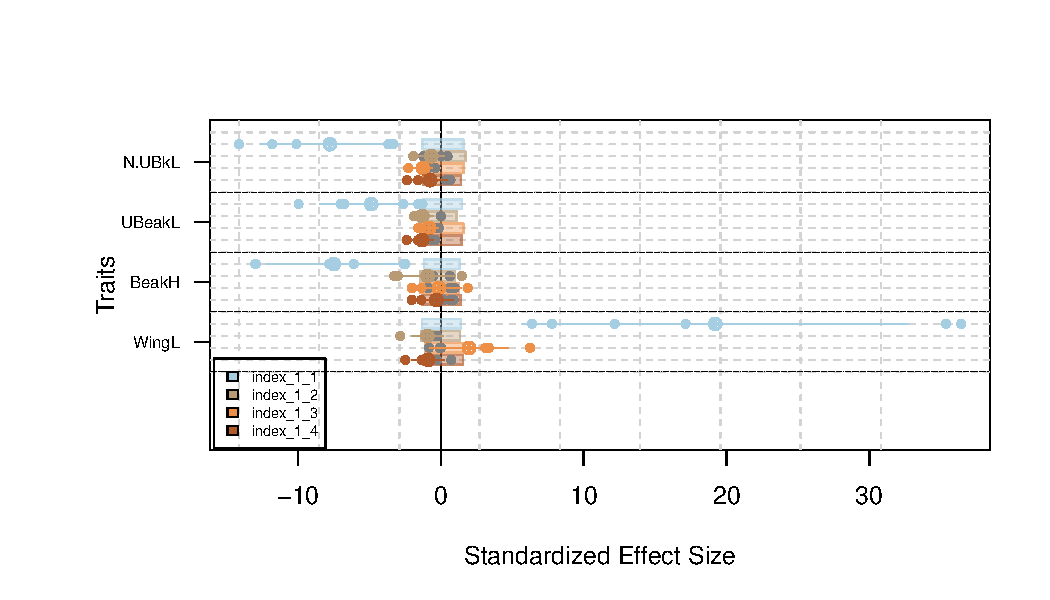
\includegraphics[width=\maxwidth]{figure/unnamed-chunk-462} 

}


=======


{\ttfamily\noindent\bfseries\color{errorcolor}{\#\# Error: objet 'res.finch.withIV' introuvable}}\begin{alltt}
\hlkwd{plot}\hlstd{(res.finch.withoutIV)}
\end{alltt}
>>>>>>> 5f89dfbb4bbfa61805f8e116f94cee418c14cfee


{\ttfamily\noindent\bfseries\color{errorcolor}{\#\# Error: objet 'res.finch.withoutIV' introuvable}}\end{kframe}
\end{knitrout}
Now plot the two analysis together.

\begin{knitrout}
\definecolor{shadecolor}{rgb}{0.969, 0.969, 0.969}\color{fgcolor}\begin{kframe}
\begin{alltt}
\hlkwd{plot}\hlstd{(}\hlkwd{as.listofindex}\hlstd{(}\hlkwd{list}\hlstd{(res.finch.withIV, res.finch.withoutIV)))}
\end{alltt}
<<<<<<< HEAD
\end{kframe}
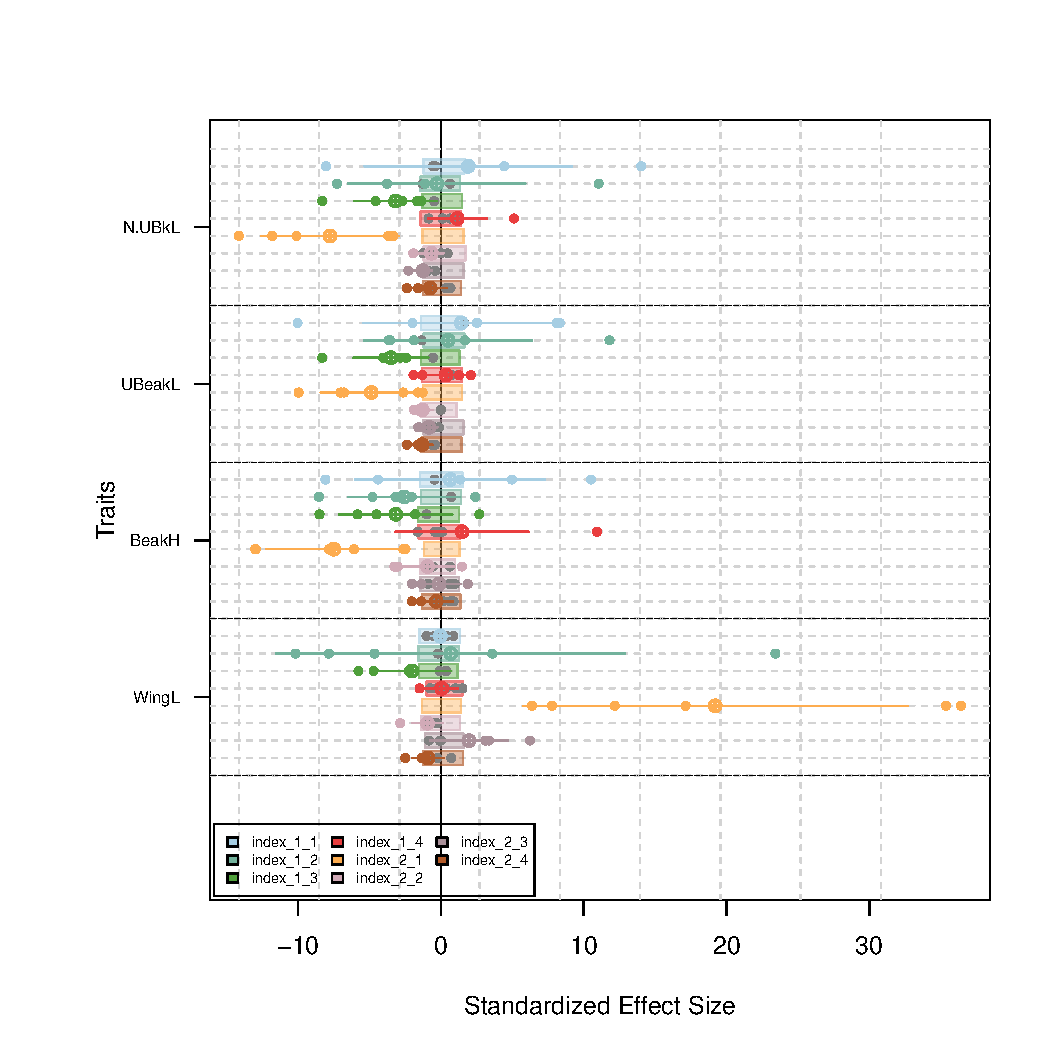
\includegraphics[width=\maxwidth]{figure/unnamed-chunk-47} 
=======
>>>>>>> 5f89dfbb4bbfa61805f8e116f94cee418c14cfee

\end{knitrout}

{\ttfamily\noindent\bfseries\color{errorcolor}{\#\# Error: objet 'res.finch.withIV' introuvable}}\end{kframe}
\end{knitrout}

\subsubsection{Plot Tstats and other uni/multivariates metrics together}
The class listofindex permits to stock different metrics computed using \texttt{Tstats}, \texttt{ComIndex} and \texttt{ComIndexMulti} and compared to different null model. To do that we can use the Standardized Effect Size (ses) define as : 

\begin{center}
$SES = (I_obs – I_sim) / \delta_{sim}$
\end{center}

where $I_obs$ is the observed value, $I_sim$ the mean of values calculated from the null model and $\delta_{sim}$ the standard deviation of these simulated values.


\begin{knitrout}
\definecolor{shadecolor}{rgb}{0.969, 0.969, 0.969}\color{fgcolor}\begin{kframe}
\begin{alltt}
\hlstd{list.ind1}\hlkwb{<-}\hlkwd{list}\hlstd{(res.finch.withIV, res.finch.withoutIV)}
\hlstd{index.list1}\hlkwb{<-}\hlkwd{as.listofindex}\hlstd{(list.ind1)}

\hlkwd{plot}\hlstd{(index.list1)}
\end{alltt}
\end{kframe}
\end{knitrout}

\begin{knitrout}
\definecolor{shadecolor}{rgb}{0.969, 0.969, 0.969}\color{fgcolor}\begin{kframe}
\begin{alltt}
\hlstd{list.ind}\hlkwb{<-}\hlkwd{list}\hlstd{(res.finch.withIV, res.finch.withoutIV, res.finch)}
\end{alltt}


{\ttfamily\noindent\bfseries\color{errorcolor}{\#\# Error: objet 'res.finch.withIV' introuvable}}\begin{alltt}
\hlstd{namesindex.i.l1} \hlkwb{=} \hlkwd{c}\hlstd{(}\hlstr{"mean"}\hlstd{,} \hlstr{"kurtosis"}\hlstd{,} \hlstr{"range"}\hlstd{,} \hlstr{"CVNND"}\hlstd{,}
         \hlstr{"mean.pop"}\hlstd{,} \hlstr{"kurtosis.pop"}\hlstd{,} \hlstr{"range.pop"}\hlstd{,} \hlstr{"CVNND.pop"}\hlstd{,}
         \hlstr{"T_IP.IC"}\hlstd{,} \hlstr{"T_IC.IR"}\hlstd{,} \hlstr{"T_PC.PR"}\hlstd{)}

\hlstd{i.l1}\hlkwb{<-}\hlkwd{as.listofindex}\hlstd{(list.ind,} \hlkwc{namesindex} \hlstd{= namesindex.i.l1)}
\end{alltt}


{\ttfamily\noindent\bfseries\color{errorcolor}{\#\# Error: objet 'list.ind' introuvable}}\begin{alltt}
\hlkwd{class}\hlstd{(i.l1)}
\end{alltt}


{\ttfamily\noindent\bfseries\color{errorcolor}{\#\# Error: objet 'i.l1' introuvable}}\end{kframe}
\end{knitrout}

The plot type \texttt{bytraits} allows plotting all SES traits values for all sites or all traits
\begin{knitrout}
\definecolor{shadecolor}{rgb}{0.969, 0.969, 0.969}\color{fgcolor}\begin{kframe}
\begin{alltt}
\hlkwd{par}\hlstd{(}\hlkwc{mfrow} \hlstd{=} \hlkwd{c}\hlstd{(}\hlnum{2}\hlstd{,}\hlnum{3}\hlstd{))}
\hlkwd{plot}\hlstd{(i.l1,}\hlkwc{type} \hlstd{=} \hlstr{"bysites"}\hlstd{)}
\end{alltt}
<<<<<<< HEAD
\end{kframe}
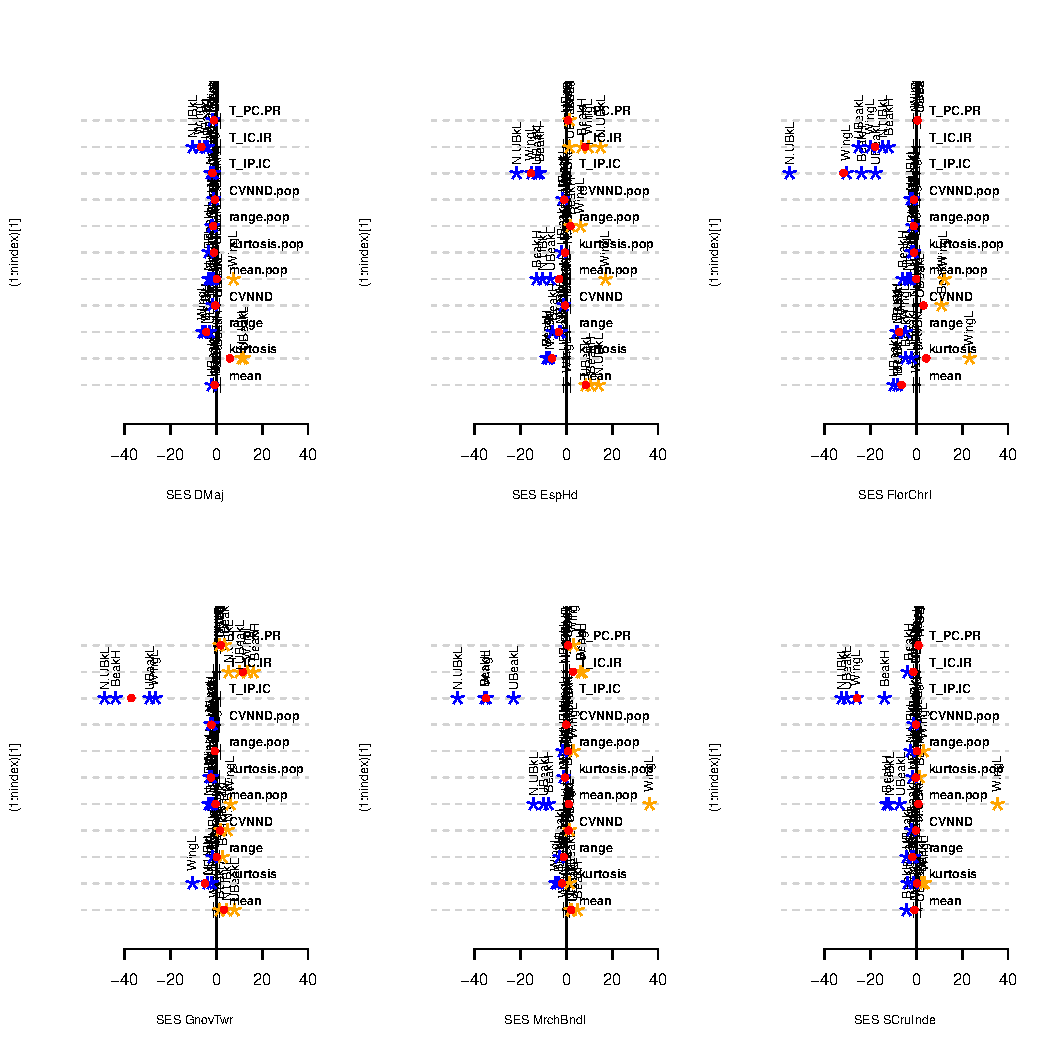
\includegraphics[width=\maxwidth]{figure/unnamed-chunk-501} 
\begin{kframe}\begin{alltt}
\hlkwd{par}\hlstd{(}\hlkwc{mfrow} \hlstd{=} \hlkwd{c}\hlstd{(}\hlnum{2}\hlstd{,}\hlnum{2}\hlstd{))}
\hlkwd{plot}\hlstd{(i.l1,}\hlkwc{type} \hlstd{=} \hlstr{"bytraits"}\hlstd{)}
\end{alltt}
\end{kframe}
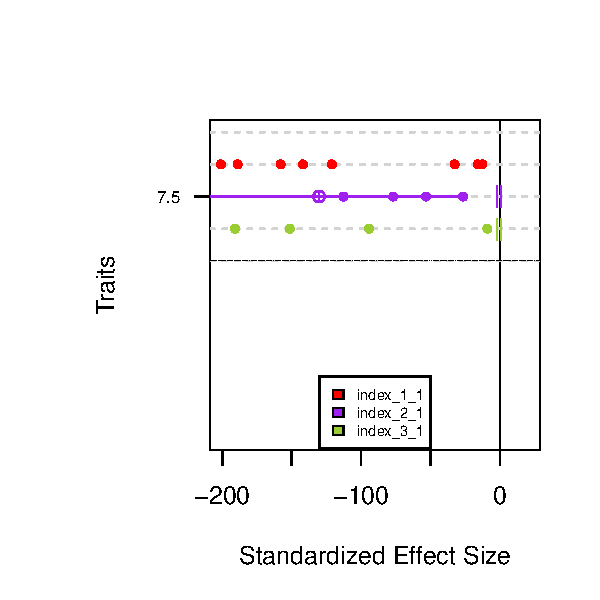
\includegraphics[width=\maxwidth]{figure/unnamed-chunk-502} 
\begin{kframe}\begin{alltt}
=======


{\ttfamily\noindent\bfseries\color{errorcolor}{\#\# Error: objet 'i.l1' introuvable}}\begin{alltt}
\hlkwd{par}\hlstd{(}\hlkwc{mfrow} \hlstd{=} \hlkwd{c}\hlstd{(}\hlnum{2}\hlstd{,}\hlnum{2}\hlstd{))}
\hlkwd{plot}\hlstd{(i.l1,}\hlkwc{type} \hlstd{=} \hlstr{"bytraits"}\hlstd{)}
\end{alltt}


{\ttfamily\noindent\bfseries\color{errorcolor}{\#\# Error: objet 'i.l1' introuvable}}\begin{alltt}
>>>>>>> 5f89dfbb4bbfa61805f8e116f94cee418c14cfee
\hlkwd{par}\hlstd{(}\hlkwc{mfrow} \hlstd{=} \hlkwd{c}\hlstd{(}\hlnum{1}\hlstd{,}\hlnum{1}\hlstd{))}
\end{alltt}
\end{kframe}
\end{knitrout}

The other plot types are the same as plot.Tstats.

\begin{knitrout}
\definecolor{shadecolor}{rgb}{0.969, 0.969, 0.969}\color{fgcolor}\begin{kframe}
\begin{alltt}
\hlkwd{plot}\hlstd{(i.l1)}
\end{alltt}
<<<<<<< HEAD
\end{kframe}
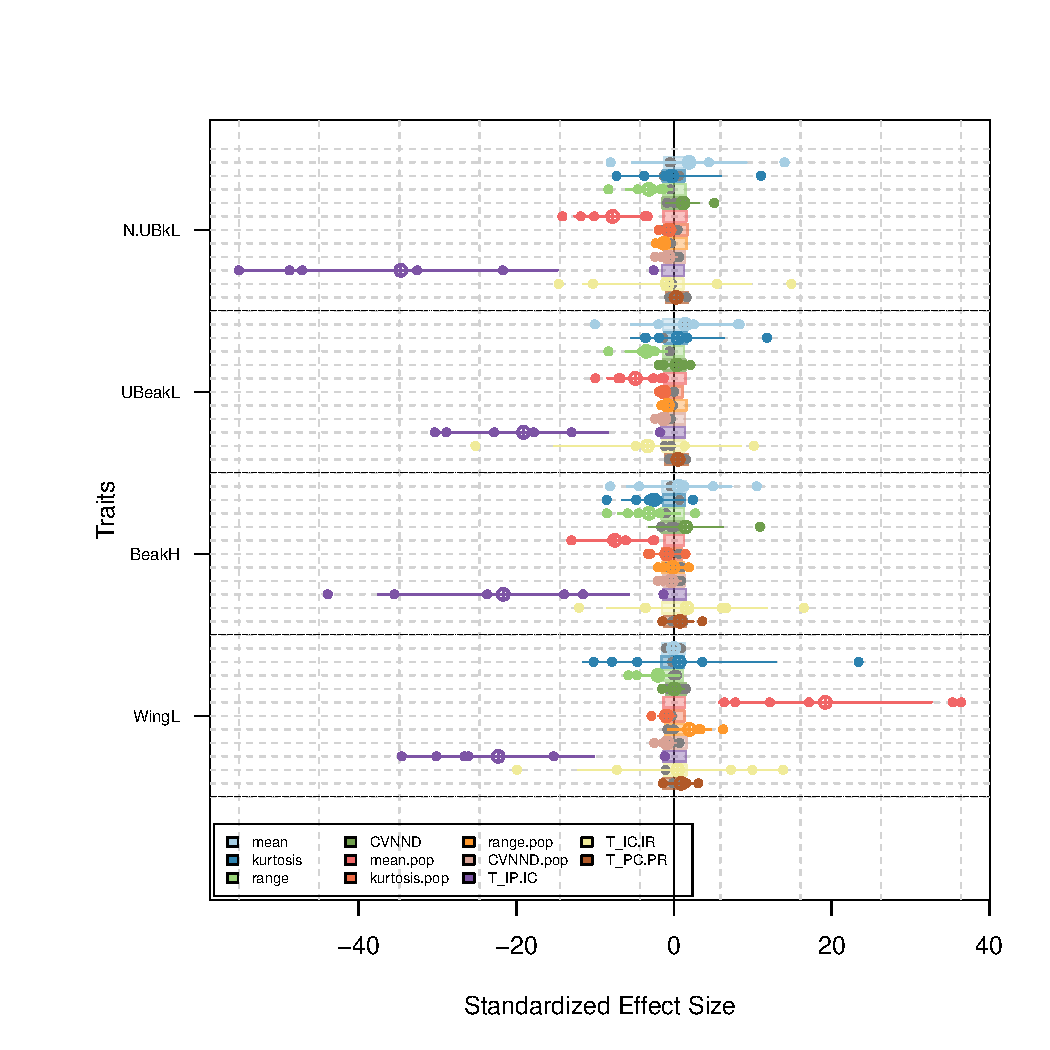
\includegraphics[width=\maxwidth]{figure/unnamed-chunk-511} 
\begin{kframe}\begin{alltt}
\hlkwd{plot}\hlstd{(i.l1,}\hlkwc{type} \hlstd{=} \hlstr{"simple_range"}\hlstd{)}
\end{alltt}
\end{kframe}

\includegraphics[width=\maxwidth]{figure/unnamed-chunk-512} 
\begin{kframe}\begin{alltt}
\hlkwd{plot}\hlstd{(i.l1,}\hlkwc{type} \hlstd{=} \hlstr{"normal"}\hlstd{)}
\end{alltt}
\end{kframe}

\includegraphics[width=\maxwidth]{figure/unnamed-chunk-513} 
\begin{kframe}\begin{alltt}
\hlkwd{plot}\hlstd{(i.l1,}\hlkwc{type} \hlstd{=} \hlstr{"barplot"}\hlstd{)}
\end{alltt}
\end{kframe}
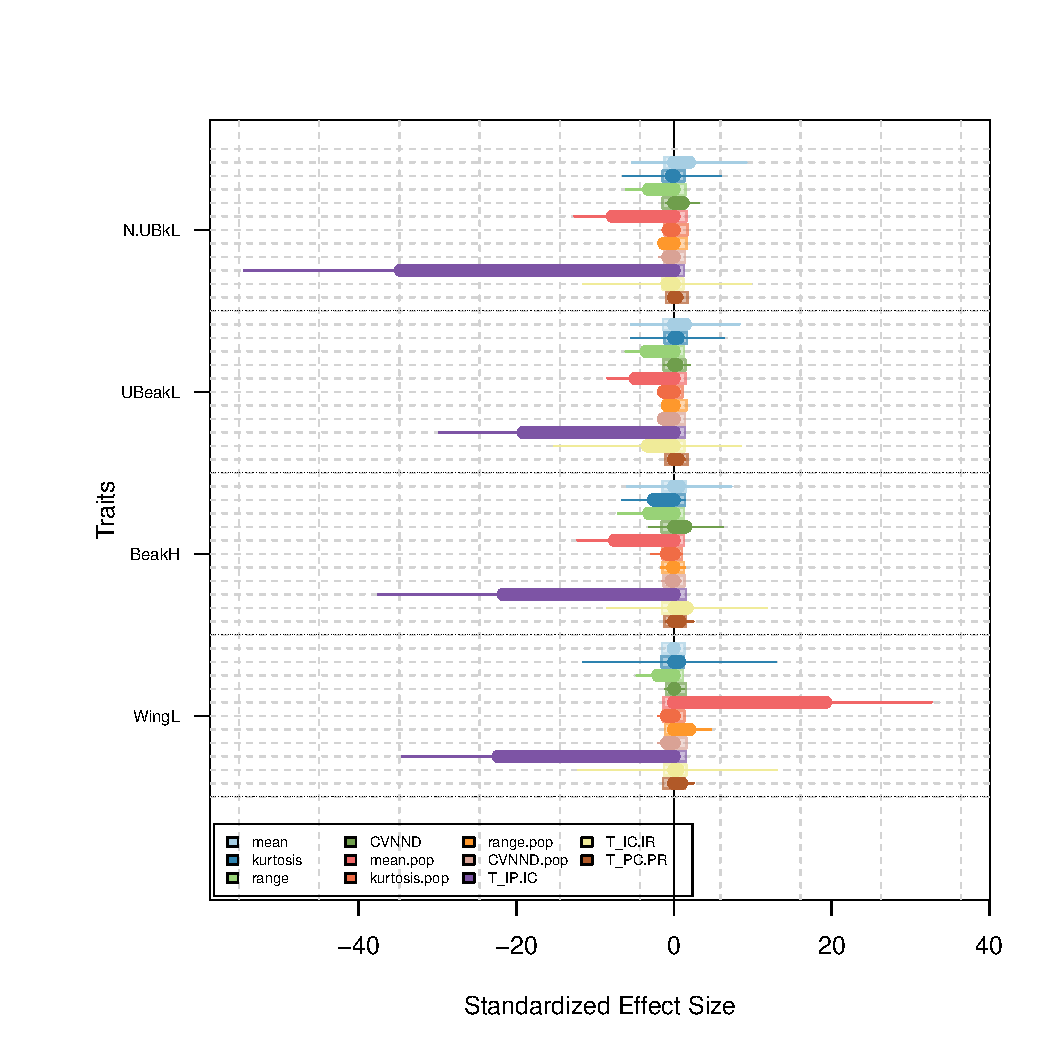
\includegraphics[width=\maxwidth]{figure/unnamed-chunk-514} 

=======


{\ttfamily\noindent\bfseries\color{errorcolor}{\#\# Error: objet 'i.l1' introuvable}}\begin{alltt}
\hlkwd{plot}\hlstd{(i.l1,}\hlkwc{type} \hlstd{=} \hlstr{"simple_range"}\hlstd{)}
\end{alltt}


{\ttfamily\noindent\bfseries\color{errorcolor}{\#\# Error: objet 'i.l1' introuvable}}\begin{alltt}
\hlkwd{plot}\hlstd{(i.l1,}\hlkwc{type} \hlstd{=} \hlstr{"normal"}\hlstd{)}
\end{alltt}


{\ttfamily\noindent\bfseries\color{errorcolor}{\#\# Error: objet 'i.l1' introuvable}}\begin{alltt}
\hlkwd{plot}\hlstd{(i.l1,}\hlkwc{type} \hlstd{=} \hlstr{"barplot"}\hlstd{)}
\end{alltt}


{\ttfamily\noindent\bfseries\color{errorcolor}{\#\# Error: objet 'i.l1' introuvable}}\begin{alltt}
\hlkwd{par}\hlstd{(}\hlkwc{mfrow} \hlstd{=} \hlkwd{c}\hlstd{(}\hlnum{1}\hlstd{,}\hlnum{1}\hlstd{))}
\end{alltt}
\end{kframe}
>>>>>>> 5f89dfbb4bbfa61805f8e116f94cee418c14cfee
\end{knitrout}



\newpage

\subsection{More information on multivariates index}

For most multivariate functions we need to replace (or exclude) NA values. For this example, we use the package \texttt{mice} to complete the data.

\begin{knitrout}
\definecolor{shadecolor}{rgb}{0.969, 0.969, 0.969}\color{fgcolor}\begin{kframe}
\begin{alltt}
\hlstd{comm}\hlkwb{<-}\hlkwd{t}\hlstd{(}\hlkwd{table}\hlstd{(ind.plot.finch,}\hlnum{1}\hlopt{:}\hlkwd{length}\hlstd{(ind.plot.finch)))}

\hlkwd{require}\hlstd{(mice)}
\hlstd{traits} \hlkwb{=} \hlstd{traits.finch}
\hlstd{mice}\hlkwb{<-}\hlkwd{mice}\hlstd{(traits.finch)}
\hlstd{traits.finch.mice}\hlkwb{<-}\hlkwd{complete}\hlstd{(mice)}
\end{alltt}
\end{kframe}
\end{knitrout}

A simple example to illustrate the concept of the function \texttt{ComIndexMulti}

\begin{knitrout}
\definecolor{shadecolor}{rgb}{0.969, 0.969, 0.969}\color{fgcolor}\begin{kframe}
\begin{alltt}
\hlstd{n_sp_plot}\hlkwb{<-}\hlkwd{as.factor}\hlstd{(}\hlkwd{paste}\hlstd{(sp.finch, ind.plot.finch,} \hlkwc{sep} \hlstd{=} \hlstr{"_"}\hlstd{))}
\hlstd{res.sum.1}\hlkwb{<-}\hlkwd{ComIndexMulti}\hlstd{(traits.finch,}
              \hlkwc{index} \hlstd{=} \hlkwd{c}\hlstd{(}\hlstr{"sum(scale(x), na.rm = T)"}\hlstd{,} \hlstr{"sum(x, na.rm = T)"}\hlstd{),}
              \hlkwc{by.factor} \hlstd{= n_sp_plot,} \hlkwc{nullmodels} \hlstd{=} \hlstr{"regional.ind"}\hlstd{,}
              \hlkwc{ind.plot} \hlstd{= ind.plot.finch,} \hlkwc{nperm} \hlstd{=} \hlnum{9}\hlstd{,} \hlkwc{sp} \hlstd{= sp.finch)}
\end{alltt}


{\ttfamily\noindent\bfseries\color{errorcolor}{\#\# Error: impossible de trouver la fonction "{}ComIndexMulti"{}}}\begin{alltt}
\hlstd{res.sum.1}
\end{alltt}
<<<<<<< HEAD
\begin{verbatim}
## 	#################################
## 	# Community metrics calculation #
## 	#################################
## class: ComIndexMulti
## $call: ComIndexMulti(traits = traits.finch, index = c("sum(scale(x), na.rm = T)", 
##     "sum(x, na.rm = T)"), by.factor = n_sp_plot, nullmodels = "regional.ind", 
##     ind.plot = ind.plot.finch, sp = sp.finch, nperm = 9)
## 
## ###############
## $obs: list of observed values
## 	$sum(scale(x), na.rm = T)
## 	$sum(x, na.rm = T)
## 
## ###############
## $null: list of null values, number of permutation: NA 
## 	$sum(scale(x), na.rm = T)_nm ... null model = regional.ind
## 	$sum(x, na.rm = T)_nm ... null model = regional.ind
## 
## ###############
## data used
##   data      class      dim   
## 1 $traits   data.frame 2513,4
## 2 $ind.plot factor     2513  
## 3 $sp       factor     2513  
##   content                                             
## 1 traits data                                         
## 2 name of the plot in which the individual is         
## 3 groups (e.g. species) which the individual belong to
## 
## ###############
## others
## 	$namestraits: 4 traits
## [1] "WingL"  "BeakH"  "UBeakL" "N.UBkL"
## 
## 	$sites_richness:
## 	    DMaj    EspHd FlorChrl  GnovTwr MrchBndl SCruInde 
##       50      267      981      258      270      687
\end{verbatim}
\end{kframe}
=======


{\ttfamily\noindent\bfseries\color{errorcolor}{\#\# Error: objet 'res.sum.1' introuvable}}\end{kframe}
>>>>>>> 5f89dfbb4bbfa61805f8e116f94cee418c14cfee
\end{knitrout}

\newpage
A more interesting example using the function \texttt{hypervolume} from the package ... \texttt{hypervolume} (Blonder et al., 2014). We show here several results which differed in there factor that delimit the group to calculate different hypervolume (argument \texttt{byfactor}). 

First, let's try the \texttt{hypervolume} function one finch data.
\begin{knitrout}
\definecolor{shadecolor}{rgb}{0.969, 0.969, 0.969}\color{fgcolor}\begin{kframe}
\begin{alltt}
\hlstd{hv}\hlkwb{<-}\hlkwd{hypervolume}\hlstd{(traits.finch.mice,}
        \hlkwc{reps} \hlstd{=} \hlnum{100}\hlstd{,}\hlkwc{bandwidth} \hlstd{=} \hlnum{0.2}\hlstd{,}
        \hlkwc{verbose} \hlstd{= F,} \hlkwc{warnings} \hlstd{= F)}
\hlkwd{plot}\hlstd{(hv)}
\end{alltt}
\end{kframe}
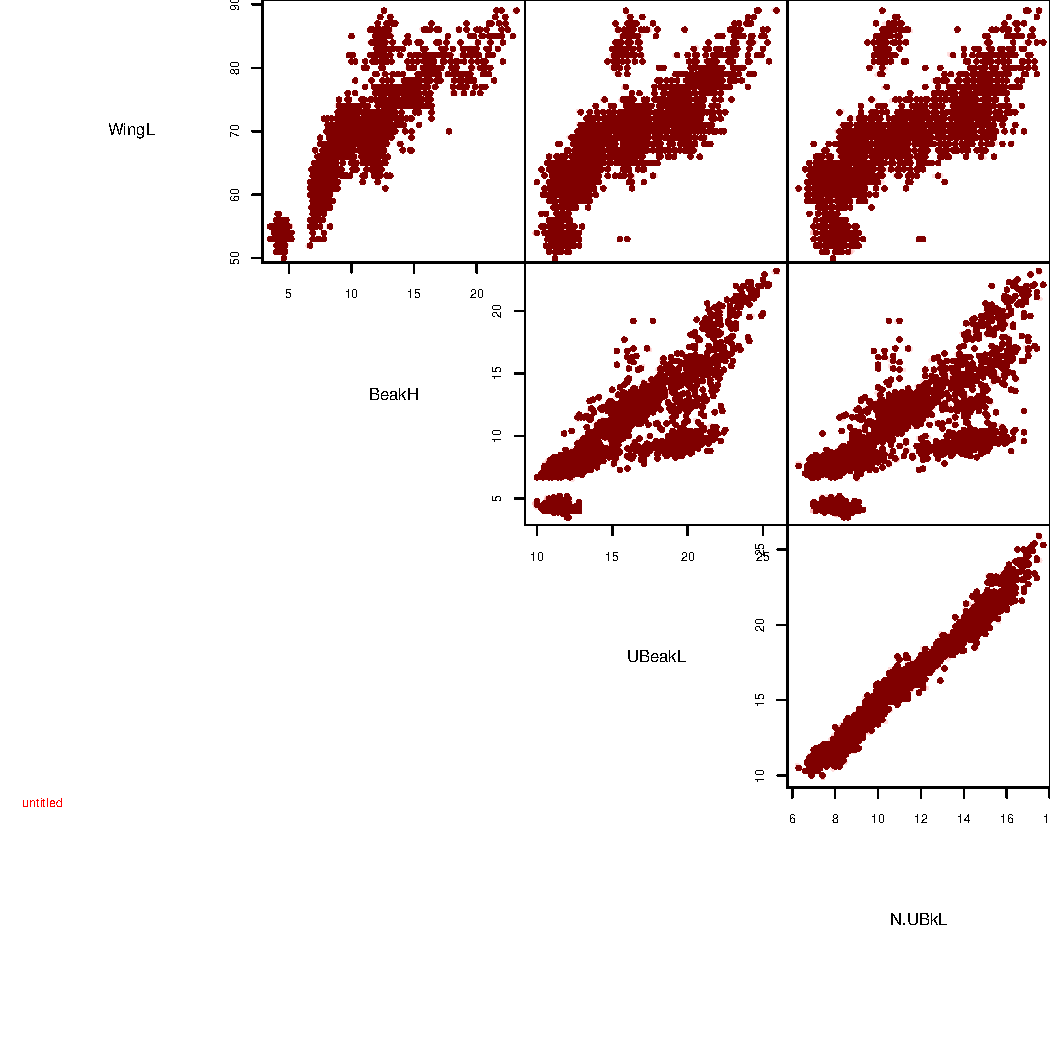
\includegraphics[width=\maxwidth]{figure/unnamed-chunk-54} 

\end{knitrout}

Now, we can do the same analysis for each species.

\begin{knitrout}
\definecolor{shadecolor}{rgb}{0.969, 0.969, 0.969}\color{fgcolor}\begin{kframe}
\begin{alltt}
\hlstd{hv.list}\hlkwb{<-}\hlkwd{new}\hlstd{(}\hlstr{"HypervolumeList"}\hlstd{)}
\hlstd{hv.list2}\hlkwb{<-}\hlkwd{list}\hlstd{()}

\hlkwa{for}\hlstd{(i} \hlkwa{in} \hlnum{1}\hlopt{:} \hlkwd{length}\hlstd{(}\hlkwd{table}\hlstd{(sp.finch))) \{}
 \hlstd{hv.list2[[i]]}\hlkwb{<-}\hlkwd{hypervolume}\hlstd{(traits.finch.mice[sp.finch} \hlopt{==} \hlkwd{levels}\hlstd{(sp.finch)[i], ],}
        \hlkwc{reps} \hlstd{=} \hlnum{1000}\hlstd{,}\hlkwc{bandwidth} \hlstd{=} \hlnum{0.2}\hlstd{,}
        \hlkwc{verbose} \hlstd{= F,} \hlkwc{warnings} \hlstd{= F)}
\hlstd{\}}

\hlstd{hv.list}\hlopt{@}\hlkwc{HVList}\hlkwb{<-}\hlstd{hv.list2}
\hlkwd{require}\hlstd{(adegenet)}
\end{alltt}


{\ttfamily\noindent\itshape\color{messagecolor}{\#\# Loading required package: adegenet\\\#\#\ \ \ \ ==========================\\\#\#\ \ \ \  adegenet 1.4-2 is loaded\\\#\#\ \ \ \ ==========================\\\#\# \\\#\#\ \ - to start, type '?adegenet'\\\#\#\ \ - to browse adegenet website, type 'adegenetWeb()'\\\#\#\ \ - to post questions/comments: adegenet-forum@lists.r-forge.r-project.org}}\begin{alltt}
\hlstd{colorhv}\hlkwb{<-}\hlkwd{transp}\hlstd{(}\hlkwd{funky}\hlstd{(}\hlkwd{nlevels}\hlstd{(sp.finch)),} \hlkwc{alpha} \hlstd{=} \hlnum{0.8}\hlstd{)}

\hlkwd{plot}\hlstd{(hv.list,} \hlkwc{colors} \hlstd{= colorhv,} \hlkwc{darkfactor} \hlstd{=} \hlnum{0.8}\hlstd{)}
\end{alltt}
\end{kframe}
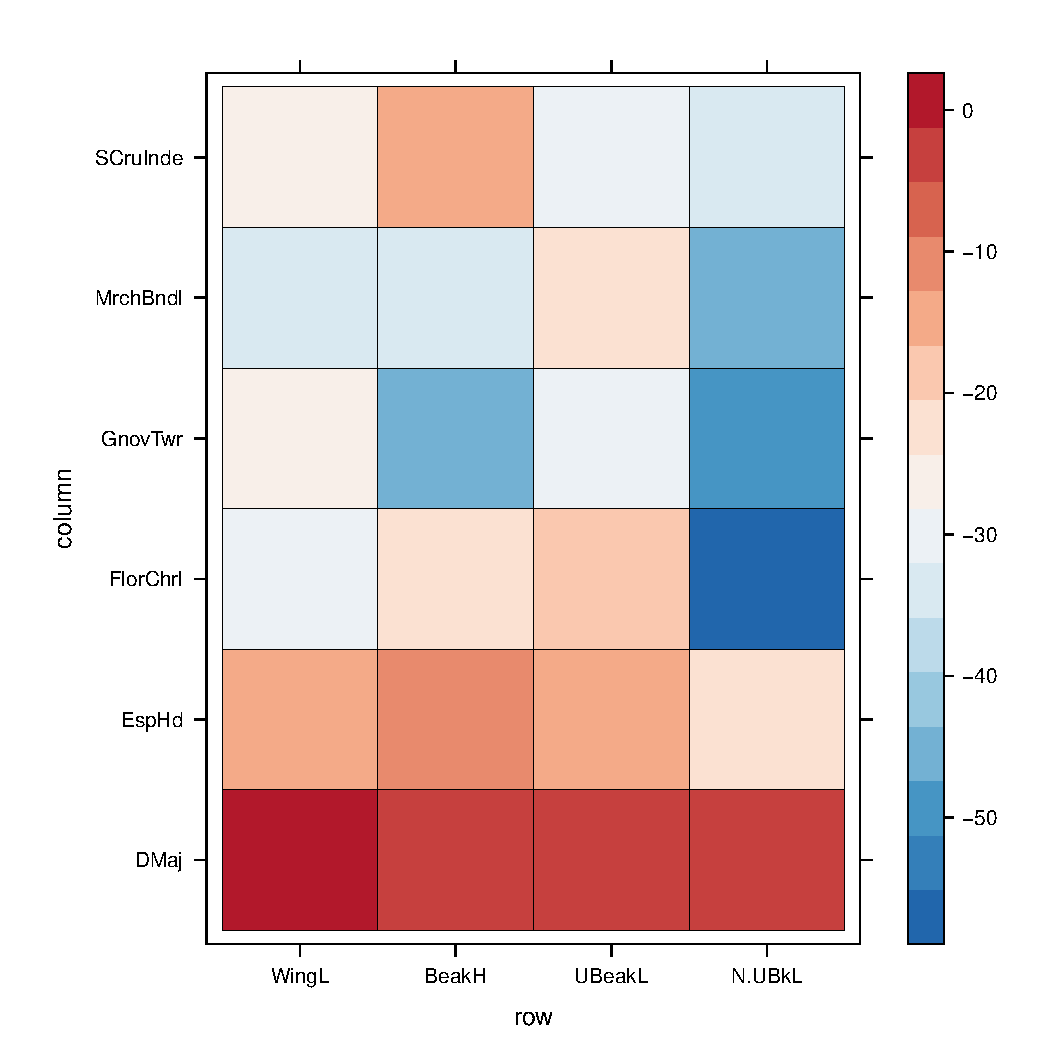
\includegraphics[width=\maxwidth]{figure/unnamed-chunk-551} 
\begin{kframe}\begin{alltt}
\hlkwd{plot}\hlstd{(hv.list,} \hlkwc{colors} \hlstd{= colorhv,} \hlkwc{darkfactor} \hlstd{=} \hlnum{0.8}\hlstd{,} \hlkwc{showdata} \hlstd{= F,} \hlkwc{npmax} \hlstd{=} \hlnum{200}\hlstd{,} \hlkwc{cex.random} \hlstd{=} \hlnum{1}\hlstd{)}
\end{alltt}
\end{kframe}
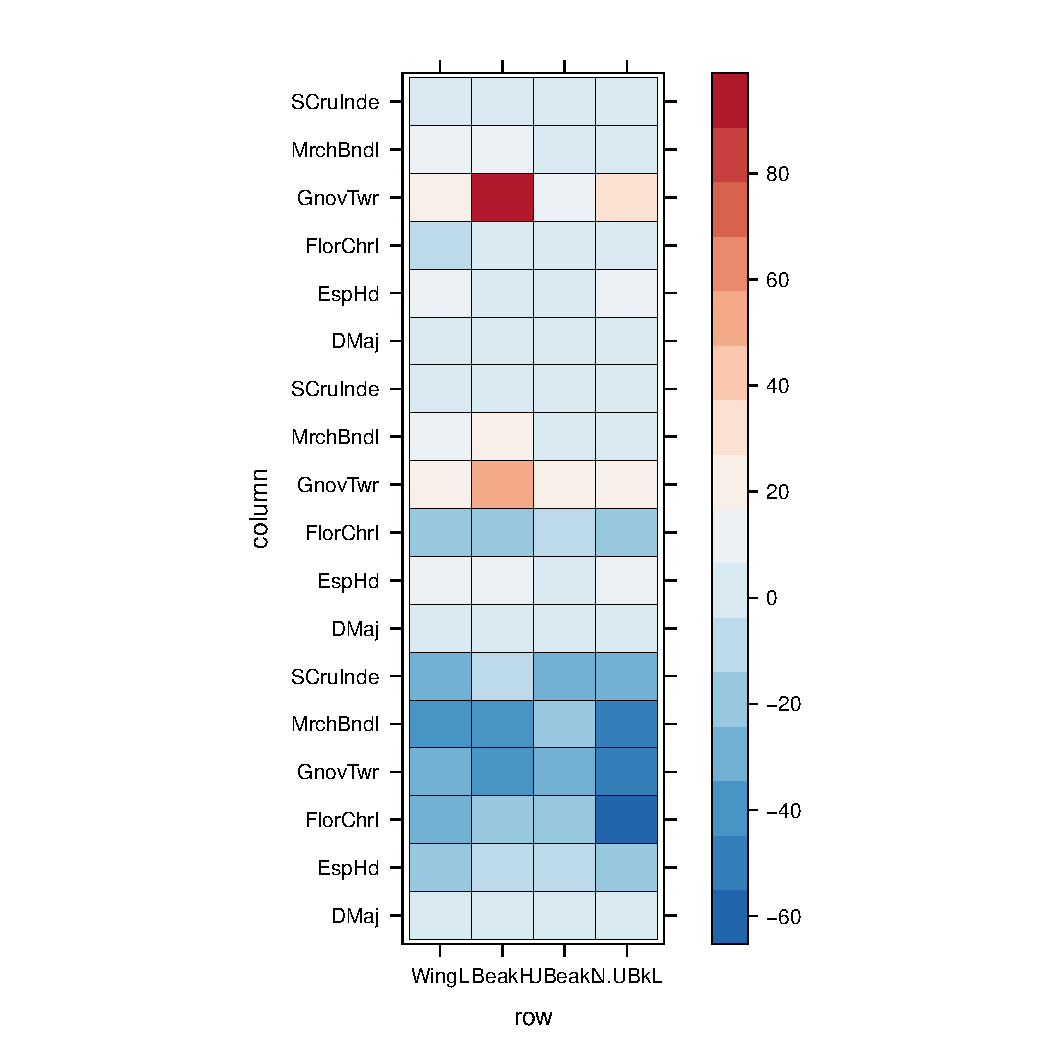
\includegraphics[width=\maxwidth]{figure/unnamed-chunk-552} 

\end{knitrout}

\begin{knitrout}
\definecolor{shadecolor}{rgb}{0.969, 0.969, 0.969}\color{fgcolor}\begin{kframe}
\begin{alltt}
\hlkwd{summary}\hlstd{(hv.list)}
\end{alltt}
\end{kframe}
\end{knitrout}

The standard example of the \texttt{hypervolume} package also use finch data but at the species level.

\begin{knitrout}
\definecolor{shadecolor}{rgb}{0.969, 0.969, 0.969}\color{fgcolor}\begin{kframe}
\begin{alltt}
\hlstd{doHypervolumeFinchDemo}\hlkwb{=}\hlnum{TRUE}
\hlkwd{demo}\hlstd{(}\hlstr{'finch'}\hlstd{,} \hlkwc{package} \hlstd{=} \hlstr{'hypervolume'}\hlstd{)}
\end{alltt}
\begin{verbatim}
## 
## 
## 	demo(finch)
## 	---- ~~~~~
## 
## > if (exists('doHypervolumeFinchDemo')==TRUE)
## + {
## +   data(finch)
## +   
## +   species_list = unique(finch$Species)
## +   num_species = length(species_list)
## +   
## +   hv_finches_list = new("HypervolumeList")
## +   hv_finches_list@HVList = vector(mode="list",length=num_species)
## +   
## +   # compute hypervolumes for each species
## +   for (i in 1:num_species)
## +   {
## +     this_species = subset(finch, Species==species_list[i])
## +     # keep the trait data
## +     this_species_log <- log10(this_species[,2:ncol(this_species)])
## +     # make a hypervolume using auto-bandwidth
## +     hv_finches_list@HVList[[i]] <- hypervolume(this_species_log, bandwidth=estimate_bandwidth(this_species_log),
## +                                                reps=10000, quantile=0, name=as.character(species_list[i]), warn=FALSE)
## +   }
## +   
## +   # compute all pairwise overlaps
## +   overlap = matrix(NA, nrow=num_species, ncol=num_species)
## +   dimnames(overlap)=list(species_list, species_list)
## +   for (i in 1:num_species)
## +   {
## +     for (j in i:num_species)
## +     {
## +       if (i!=j)
## +       {
## +         # compute set operations on each pair
## +         this_set = hypervolume_set(hv_finches_list@HVList[[i]], hv_finches_list@HVList[[j]],reduction_factor=0.5, check_memory=FALSE)
## +         # calculate a Sorensen overlap index (2 x shared volume / sum of |hv1| + |hv2|)
## +         overlap[i,j] = 2 * this_set@HVList$Intersection@Volume / (hv_finches_list@HVList[[i]]@Volume + hv_finches_list@HVList[[j]]@Volume)
## +       }
## +     }   
## +   }
## +   
## + 
## +   
## +   # show all hypervolumes
## +   plot(hv_finches_list,npmax=500,darkfactor=0.5,cex.legend=0.25,cex.names=0.75)
## +   
## +   # show pairwise overlaps - note that actually very few species overlap in nine dimensions
## +   op <- par(mar=c(10,10,1,1))
## +   image(x=1:nrow(overlap), y=1:nrow(overlap), z=overlap,axes=F,xlab='',ylab='',col=rainbow(5))
## +   box()
## +   axis(side=1, at=1:(length(dimnames(overlap)[[1]])),dimnames(overlap)[[1]],las=2,cex.axis=0.75)
## +   axis(side=2, at=1:(length(dimnames(overlap)[[2]])),dimnames(overlap)[[2]],las=1,cex.axis=0.75)
## +   par(op)
## +   
## +   rm(doHypervolumeFinchDemo)
## + } else
## + {
## +   message('Demo does not run by default to meet CRAN runtime requirements.')
## +   message('This demo requires approximately 3 minutes to run.')  
## +   message('To run the demo, type')
## +   message('\tdoHypervolumeFinchDemo=TRUE')
## +   message('\tdemo(finch)')
## +   message('at the R command line prompt.')
## + }
## Evaluating probability density...
## Building tree... done.
## Querying tree... 5.26316e-006  0.0526368  0.105268  0.1579  0.210532  0.263163  0.315795  0.368426  0.421058  0.473689  0.526321  0.578953  0.631584  0.684216  0.736847  0.789479  0.842111  0.894742  0.947374  done.
## Finished evaluating probability density.
## Beginning volume calculation... done. 
## Quantile requested: 0.00   obtained: 0.00
## Evaluating probability density...
## Building tree... done.
## Querying tree... 7.69231e-006  0.0769308  0.153854  0.230777  0.3077  0.384623  0.461546  0.538469  0.615392  0.692315  0.769238  0.846162  0.923085  done.
## Finished evaluating probability density.
## Beginning volume calculation... done. 
## Quantile requested: 0.00   obtained: 0.00
## Evaluating probability density...
## Building tree... done.
## Querying tree... 1.23457e-006  0.0123469  0.0246926  0.0370383  0.049384  0.0617296  0.0740753  0.086421  0.0987667  0.111112  0.123458  0.135804  0.148149  0.160495  0.172841  0.185186  0.197532  0.209878  0.222223  0.234569  0.246915  0.25926  0.271606  0.283952  0.296298  0.308643  0.320989  0.333335  0.34568  0.358026  0.370372  0.382717  0.395063  0.407409  0.419754  0.4321  0.444446  0.456791  0.469137  0.481483  0.493828  0.506174  0.51852  0.530865  0.543211  0.555557  0.567902  0.580248  0.592594  0.60494  0.617285  0.629631  0.641977  0.654322  0.666668  0.679014  0.691359  0.703705  0.716051  0.728396  0.740742  0.753088  0.765433  0.777779  0.790125  0.80247  0.814816  0.827162  0.839507  0.851853  0.864199  0.876544  0.88889  0.901236  0.913581  0.925927  0.938273  0.950619  0.962964  0.97531  0.987656  done.
## Finished evaluating probability density.
## Beginning volume calculation... done. 
## Quantile requested: 0.00   obtained: 0.00
## Evaluating probability density...
## Building tree... done.
## Querying tree... 4.54545e-006  0.0454591  0.0909136  0.136368  0.181823  0.227277  0.272732  0.318186  0.363641  0.409095  0.45455  0.500005  0.545459  0.590914  0.636368  0.681823  0.727277  0.772732  0.818186  0.863641  0.909095  0.95455  done.
## Finished evaluating probability density.
## Beginning volume calculation... done. 
## Quantile requested: 0.00   obtained: 0.00
## Evaluating probability density...
## Building tree... done.
## Querying tree... 9.09091e-006  0.0909182  0.181827  0.272736  0.363645  0.454555  0.545464  0.636373  0.727282  0.818191  0.9091  done.
## Finished evaluating probability density.
## Beginning volume calculation... done. 
## Quantile requested: 0.00   obtained: 0.00
## Retaining 30687 points in hv1 and 39679 points in hv2.
## Beginning ball queries... 
## Building tree... done.
## Querying tree... 2.52022e-005  0.252048  0.50407  0.756093  done.
## Building tree... done.
## Querying tree... 3.25871e-005  0.325903  0.651774  0.977645  done.
## Finished ball queries. 
## Retaining 57681 points in hv1 and 56195 points in hv2.
## Beginning ball queries... 
## Building tree... done.
## Querying tree... 1.77952e-005  0.17797  0.355921  0.533873  0.711825  0.889777  done.
## Building tree... done.
## Querying tree... 1.73367e-005  0.173385  0.346752  0.520119  0.693487  0.866854  done.
## Finished ball queries. 
## Retaining 1264 points in hv1 and 61558 points in hv2.
## Beginning ball queries... 
## Building tree... done.
## Querying tree... 1.62448e-005  0.162465  0.324913  0.487362  0.64981  0.812258  0.974707  done.
## Building tree... done.
## Querying tree... 0.000791139  done.
## Finished ball queries. 
## Retaining 428 points in hv1 and 31481 points in hv2.
## Beginning ball queries... 
## Building tree... done.
## Querying tree... 3.17652e-005  0.317684  0.635336  0.952988  done.
## Building tree... done.
## Querying tree... 0.00233645  done.
## Finished ball queries. 
## Retaining 39679 points in hv1 and 29896 points in hv2.
## Beginning ball queries... 
## Building tree... done.
## Querying tree... 3.34493e-005  0.334526  0.669019  done.
## Building tree... done.
## Querying tree... 2.52022e-005  0.252048  0.50407  0.756093  done.
## Finished ball queries. 
## Retaining 1635 points in hv1 and 61558 points in hv2.
## Beginning ball queries... 
## Building tree... done.
## Querying tree... 1.62448e-005  0.162465  0.324913  0.487362  0.64981  0.812258  0.974707  done.
## Building tree... done.
## Querying tree... 0.000611621  done.
## Finished ball queries. 
## Retaining 553 points in hv1 and 31481 points in hv2.
## Beginning ball queries... 
## Building tree... done.
## Querying tree... 3.17652e-005  0.317684  0.635336  0.952988  done.
## Building tree... done.
## Querying tree... 0.00180832  done.
## Finished ball queries. 
## Retaining 1232 points in hv1 and 61558 points in hv2.
## Beginning ball queries... 
## Building tree... done.
## Querying tree... 1.62448e-005  0.162465  0.324913  0.487362  0.64981  0.812258  0.974707  done.
## Building tree... done.
## Querying tree... 0.000811688  done.
## Finished ball queries. 
## Retaining 416 points in hv1 and 31481 points in hv2.
## Beginning ball queries... 
## Building tree... done.
## Querying tree... 3.17652e-005  0.317684  0.635336  0.952988  done.
## Building tree... done.
## Querying tree... 0.00240385  done.
## Finished ball queries. 
## Retaining 20829 points in hv1 and 31481 points in hv2.
## Beginning ball queries... 
## Building tree... done.
## Querying tree... 3.17652e-005  0.317684  0.635336  0.952988  done.
## Building tree... done.
## Querying tree... 4.801e-005  0.480148  0.960248  done.
## Finished ball queries.
\end{verbatim}
\end{kframe}
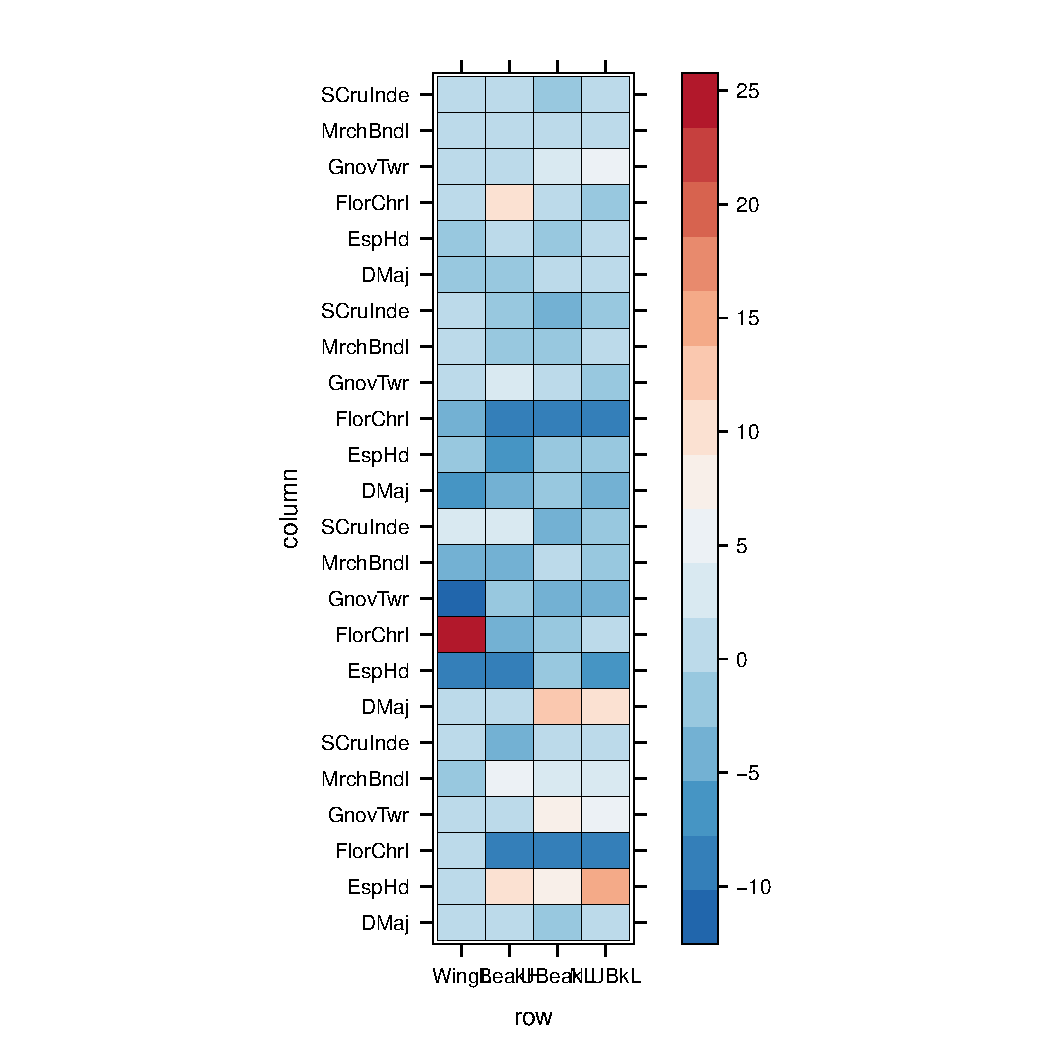
\includegraphics[width=\maxwidth]{figure/unnamed-chunk-571} 

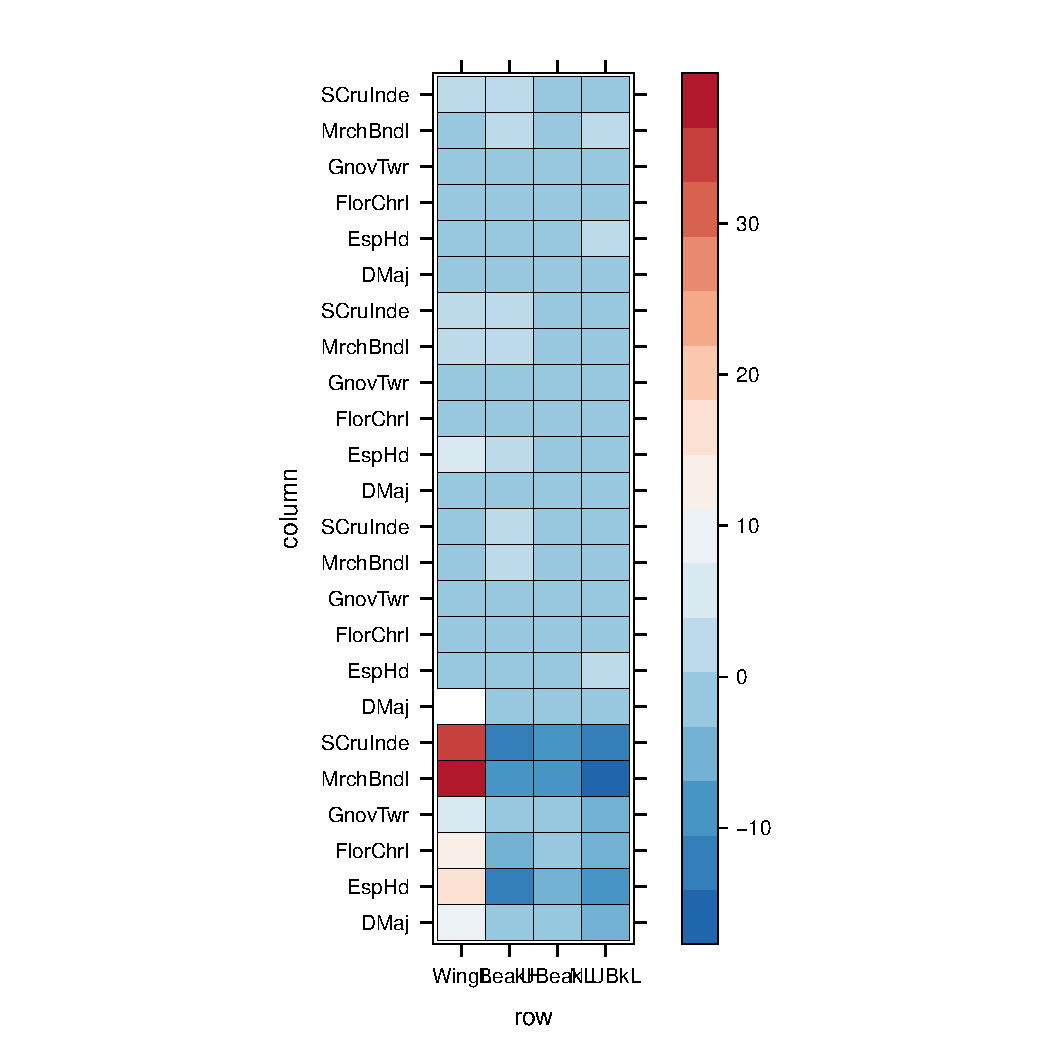
\includegraphics[width=\maxwidth]{figure/unnamed-chunk-572} 

\end{knitrout}
End of Hypervolume finch demo

\texttt{ComIndexMulti} takes the same arguments as \texttt{ComIndex} and an argument by factor to apply the index on different factors.

\begin{knitrout}
\definecolor{shadecolor}{rgb}{0.969, 0.969, 0.969}\color{fgcolor}\begin{kframe}
\begin{alltt}
\hlcom{#all individual are put in the same group: calculate the hypervolume without by.factor}
\hlstd{hv.1}\hlkwb{<-}\hlkwd{ComIndexMulti}\hlstd{(traits.finch.mice,}
             \hlkwc{index} \hlstd{=} \hlkwd{c}\hlstd{(}\hlstr{"as.numeric(try(hypervolume(na.omit(x), reps = 100, 
                 bandwidth = 0.2, verbose = F, warnings = F)@Volume))"}\hlstd{),}
             \hlkwc{by.factor} \hlstd{=} \hlkwd{rep}\hlstd{(}\hlnum{1}\hlstd{,}\hlkwd{length}\hlstd{(n_sp_plot)),} \hlkwc{nullmodels} \hlstd{=} \hlstr{"regional.ind"}\hlstd{,}
             \hlkwc{ind.plot} \hlstd{= ind.plot.finch,} \hlkwc{nperm} \hlstd{=} \hlnum{9}\hlstd{,} \hlkwc{sp} \hlstd{= sp.finch)}
\end{alltt}


{\ttfamily\noindent\bfseries\color{errorcolor}{\#\# Error: impossible de trouver la fonction "{}ComIndexMulti"{}}}\begin{alltt}
\hlstd{hv.2}\hlkwb{<-}\hlkwd{ComIndexMulti}\hlstd{(traits.finch.mice,}
             \hlkwc{index} \hlstd{=} \hlkwd{c}\hlstd{(}\hlstr{"as.numeric(try(hypervolume(na.omit(x), reps = 100, 
                 bandwidth = 0.2, verbose = F, warnings = F)@Volume))"}\hlstd{),}
             \hlkwc{by.factor} \hlstd{= n_sp_plot,} \hlkwc{nullmodels} \hlstd{=} \hlstr{"regional.ind"}\hlstd{,}
             \hlkwc{ind.plot} \hlstd{= ind.plot.finch,} \hlkwc{nperm} \hlstd{=} \hlnum{9}\hlstd{,} \hlkwc{sp} \hlstd{= sp.finch,} \hlkwc{print} \hlstd{=} \hlnum{FALSE}\hlstd{)}
\end{alltt}


<<<<<<< HEAD
=======
{\ttfamily\noindent\bfseries\color{errorcolor}{\#\# Error: impossible de trouver la fonction "{}ComIndexMulti"{}}}\begin{alltt}
>>>>>>> 5f89dfbb4bbfa61805f8e116f94cee418c14cfee
\hlstd{hv.3}\hlkwb{<-}\hlkwd{ComIndexMulti}\hlstd{(traits.finch.mice,}
             \hlkwc{index} \hlstd{=} \hlkwd{c}\hlstd{(}\hlstr{"as.numeric(try(hypervolume(na.omit(x), reps = 100,
                 bandwidth = 0.2, verbose = F, warnings = F)@Volume))"}\hlstd{),}
             \hlkwc{by.factor} \hlstd{= ind.plot.finch,} \hlkwc{nullmodels} \hlstd{=}\hlstr{"regional.ind"}\hlstd{,}
             \hlkwc{ind.plot} \hlstd{= ind.plot.finch,} \hlkwc{nperm} \hlstd{=} \hlnum{9}\hlstd{,} \hlkwc{sp} \hlstd{= sp.finch,} \hlkwc{print} \hlstd{=} \hlnum{FALSE}\hlstd{)}
\end{alltt}


<<<<<<< HEAD
=======
{\ttfamily\noindent\bfseries\color{errorcolor}{\#\# Error: impossible de trouver la fonction "{}ComIndexMulti"{}}}\begin{alltt}
>>>>>>> 5f89dfbb4bbfa61805f8e116f94cee418c14cfee
\hlstd{hv.4}\hlkwb{<-}\hlkwd{ComIndexMulti}\hlstd{(traits.finch.mice,}
             \hlkwc{index} \hlstd{=} \hlkwd{c}\hlstd{(}\hlstr{"as.numeric(try(hypervolume(na.omit(x), reps = 100, 
                 bandwidth = 0.2, verbose = F, warnings = F)@Volume))"}\hlstd{),}
             \hlkwc{by.factor} \hlstd{= sp.finch,} \hlkwc{nullmodels} \hlstd{=} \hlstr{"regional.ind"}\hlstd{,}
             \hlkwc{ind.plot} \hlstd{= ind.plot.finch,} \hlkwc{nperm} \hlstd{=} \hlnum{9}\hlstd{,} \hlkwc{sp} \hlstd{= sp.finch,} \hlkwc{print} \hlstd{=} \hlnum{FALSE}\hlstd{)}
\end{alltt}


<<<<<<< HEAD
=======
{\ttfamily\noindent\bfseries\color{errorcolor}{\#\# Error: impossible de trouver la fonction "{}ComIndexMulti"{}}}\begin{alltt}
>>>>>>> 5f89dfbb4bbfa61805f8e116f94cee418c14cfee
\hlstd{list.ind.multi}\hlkwb{<-}\hlkwd{as.listofindex}\hlstd{(}\hlkwd{list}\hlstd{(hv.2, hv.3, hv.4))}
\end{alltt}


{\ttfamily\noindent\bfseries\color{errorcolor}{\#\# Error: objet 'hv.2' introuvable}}\begin{alltt}
\hlstd{ses.list.multi}\hlkwb{<-}\hlkwd{ses.listofindex}\hlstd{(list.ind.multi)}
\end{alltt}


{\ttfamily\noindent\bfseries\color{errorcolor}{\#\# Error: objet 'list.ind.multi' introuvable}}\begin{alltt}
\hlstd{ses.list.multi}
\end{alltt}


{\ttfamily\noindent\bfseries\color{errorcolor}{\#\# Error: objet 'ses.list.multi' introuvable}}\end{kframe}
\end{knitrout}

\begin{knitrout}
\definecolor{shadecolor}{rgb}{0.969, 0.969, 0.969}\color{fgcolor}\begin{kframe}
\begin{alltt}
\hlkwd{plot}\hlstd{(list.ind.multi)}
\end{alltt}
<<<<<<< HEAD
\end{kframe}

{\centering 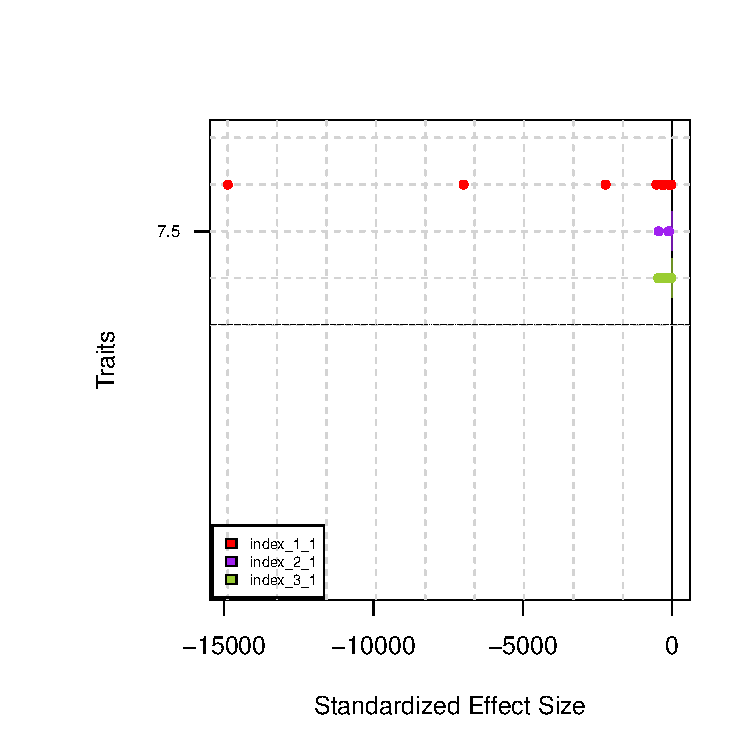
\includegraphics[width=\maxwidth]{figure/unnamed-chunk-591} 
=======

>>>>>>> 5f89dfbb4bbfa61805f8e116f94cee418c14cfee

{\ttfamily\noindent\bfseries\color{errorcolor}{\#\# Error: erreur d'évaluation de l'argument 'x' lors de la sélection d'une méthode pour la fonction 'plot' : Erreur : objet 'list.ind.multi' introuvable}}\begin{alltt}
\hlcom{#Try a zoom on the area near zero}
\hlkwd{plot}\hlstd{(list.ind.multi,} \hlkwc{xlim} \hlstd{=} \hlkwd{c}\hlstd{(}\hlopt{-}\hlnum{200}\hlstd{,}\hlnum{20}\hlstd{))}
\end{alltt}
<<<<<<< HEAD
\end{kframe}

{\centering 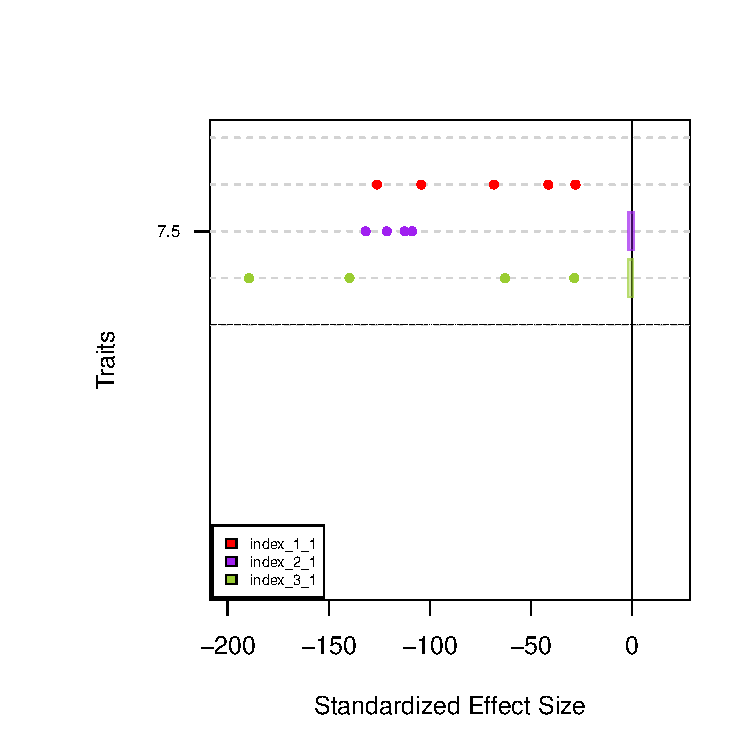
\includegraphics[width=\maxwidth]{figure/unnamed-chunk-592} 

}



=======


{\ttfamily\noindent\bfseries\color{errorcolor}{\#\# Error: erreur d'évaluation de l'argument 'x' lors de la sélection d'une méthode pour la fonction 'plot' : Erreur : objet 'list.ind.multi' introuvable}}\end{kframe}
>>>>>>> 5f89dfbb4bbfa61805f8e116f94cee418c14cfee
\end{knitrout}

Compare hypervolume to Villéger's metrics convex hull.

\begin{knitrout}
\definecolor{shadecolor}{rgb}{0.969, 0.969, 0.969}\color{fgcolor}\begin{kframe}
\begin{alltt}
\hlkwd{require}\hlstd{(}\hlstr{"geometry"}\hlstd{)}
\end{alltt}


{\ttfamily\noindent\itshape\color{messagecolor}{\#\# Loading required package: geometry\\\#\# Loading required package: magic\\\#\# Loading required package: abind}}\begin{alltt}
\hlstd{FA}\hlkwb{<-}\hlkwd{as.character}\hlstd{(}\hlstr{"FA"}\hlstd{)}
\hlstd{funct}\hlkwb{<-}\hlkwd{c}\hlstd{(}\hlstr{"round(convhulln(x,FA)$vol,6)"}\hlstd{)}

\hlcom{##Null model local is trivial for this function}
\hlcom{##because randomization is within community only}
\hlstd{Fdis.finch}\hlkwb{<-}\hlkwd{ComIndexMulti}\hlstd{(traits.finch.mice,}
             \hlkwc{index} \hlstd{= funct,}
             \hlkwc{by.factor} \hlstd{= ind.plot.finch,} \hlkwc{nullmodels} \hlstd{=} \hlstr{"local"}\hlstd{,}
             \hlkwc{ind.plot} \hlstd{= ind.plot.finch,} \hlkwc{nperm} \hlstd{=} \hlnum{9}\hlstd{,} \hlkwc{sp} \hlstd{= sp.finch)}
\end{alltt}


{\ttfamily\noindent\bfseries\color{errorcolor}{\#\# Error: impossible de trouver la fonction "{}ComIndexMulti"{}}}\begin{alltt}
\hlstd{list.ind.multi2}\hlkwb{<-}\hlkwd{as.listofindex}\hlstd{(}\hlkwd{list}\hlstd{(hv.3, Fdis.finch))}
\end{alltt}


{\ttfamily\noindent\bfseries\color{errorcolor}{\#\# Error: objet 'hv.3' introuvable}}\begin{alltt}
\hlstd{ses.list.multi2}\hlkwb{<-}\hlkwd{ses.listofindex}\hlstd{(list.ind.multi2)}
\end{alltt}


{\ttfamily\noindent\bfseries\color{errorcolor}{\#\# Error: objet 'list.ind.multi2' introuvable}}\end{kframe}
\end{knitrout}

\begin{knitrout}
\definecolor{shadecolor}{rgb}{0.969, 0.969, 0.969}\color{fgcolor}\begin{kframe}
\begin{alltt}
\hlkwd{plot}\hlstd{(list.ind.multi2)}
\end{alltt}
<<<<<<< HEAD
\end{kframe}
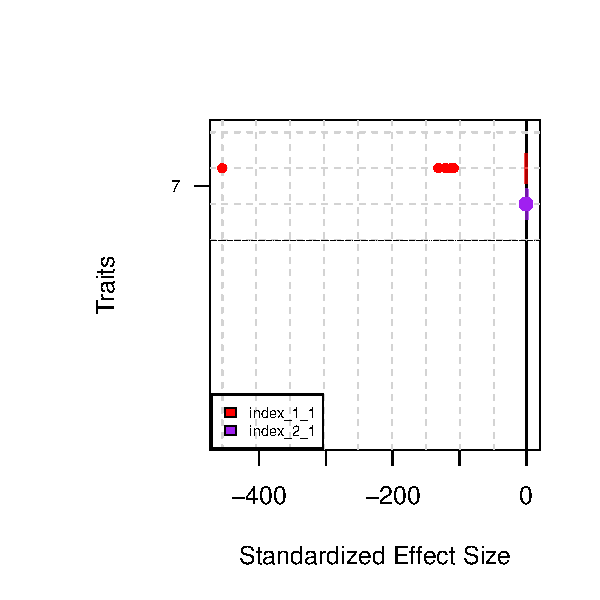
\includegraphics[width=\maxwidth]{figure/unnamed-chunk-61} 
=======
>>>>>>> 5f89dfbb4bbfa61805f8e116f94cee418c14cfee


{\ttfamily\noindent\bfseries\color{errorcolor}{\#\# Error: erreur d'évaluation de l'argument 'x' lors de la sélection d'une méthode pour la fonction 'plot' : Erreur : objet 'list.ind.multi2' introuvable}}\end{kframe}
\end{knitrout}

\section{Others graphical functions}

Use rasterVis to obtain more color schemes. 
\begin{knitrout}
\definecolor{shadecolor}{rgb}{0.969, 0.969, 0.969}\color{fgcolor}\begin{kframe}


{\ttfamily\noindent\itshape\color{messagecolor}{\#\# Loading required package: rasterVis\\\#\# Loading required package: raster\\\#\# Loading required package: sp\\\#\# \\\#\# Attaching package: 'raster'\\\#\# \\\#\# The following object is masked from 'package:magic':\\\#\# \\\#\#\ \ \ \  shift\\\#\# \\\#\# The following objects are masked from 'package:ape':\\\#\# \\\#\#\ \ \ \  rotate, zoom\\\#\# \\\#\# The following object is masked from 'package:nlme':\\\#\# \\\#\#\ \ \ \  getData\\\#\# \\\#\# Loading required package: latticeExtra\\\#\# Loading required package: RColorBrewer\\\#\# Loading required package: hexbin}}\end{kframe}
\end{knitrout}

Plot the p-value or the ses values using the function \texttt{levelplot}.

\begin{knitrout}
\definecolor{shadecolor}{rgb}{0.969, 0.969, 0.969}\color{fgcolor}\begin{kframe}
\begin{alltt}
\hlkwd{levelplot}\hlstd{(}\hlkwd{t}\hlstd{(}\hlkwd{sum_Tstats}\hlstd{(res.finch)}\hlopt{$}\hlstd{p.value),}
     \hlkwc{colorkey} \hlstd{= my.ckey,} \hlkwc{par.settings} \hlstd{= my.theme,}\hlkwc{border} \hlstd{=} \hlstr{"black"}\hlstd{)}
\end{alltt}
<<<<<<< HEAD
\end{kframe}
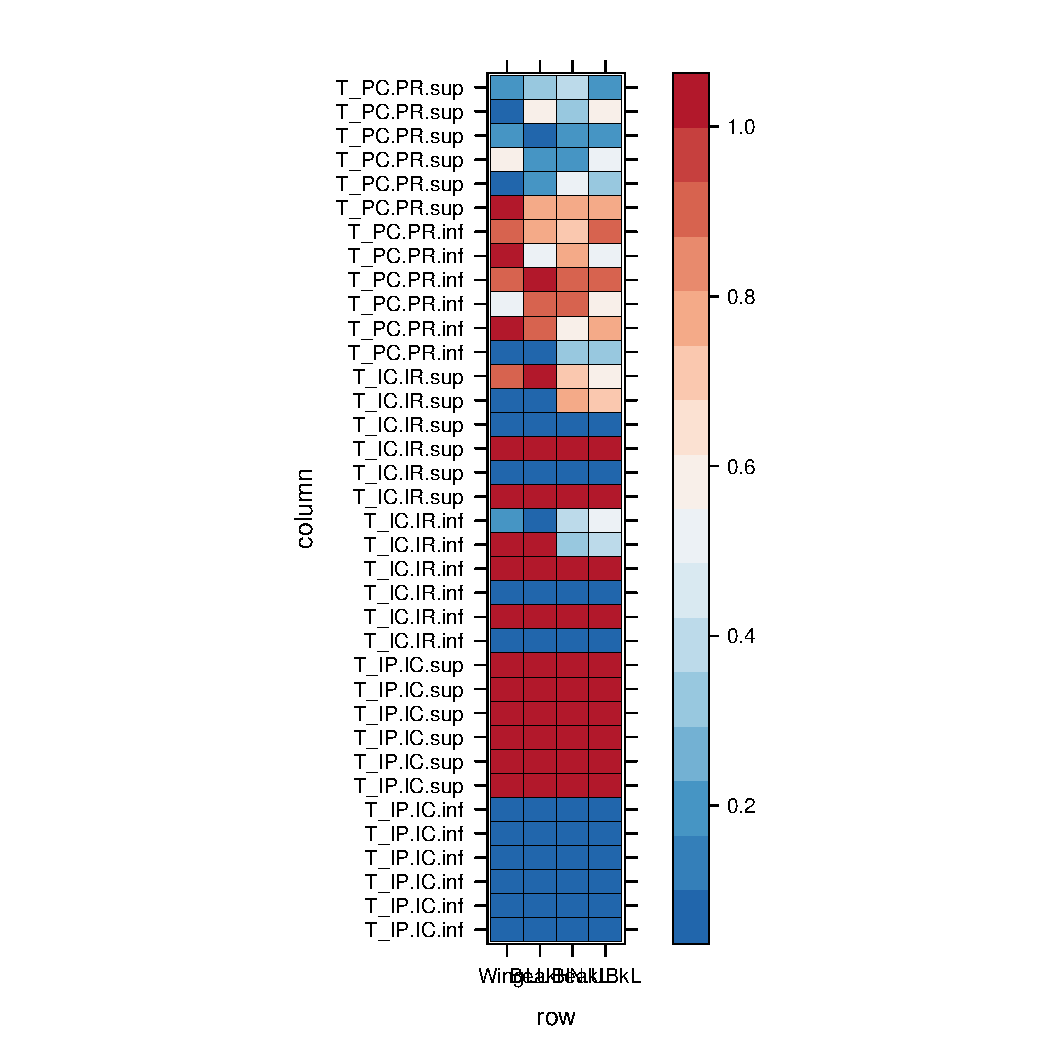
\includegraphics[width=\maxwidth]{figure/unnamed-chunk-63} 
=======
>>>>>>> 5f89dfbb4bbfa61805f8e116f94cee418c14cfee


{\ttfamily\noindent\bfseries\color{errorcolor}{\#\# Error: erreur d'évaluation de l'argument 'x' lors de la sélection d'une méthode pour la fonction 'levelplot' : Erreur dans t(sum\_Tstats(res.finch)\$p.value) : \\\#\#\ \  erreur d'évaluation de l'argument 'x' lors de la sélection d'une méthode pour la fonction 't' : Erreur : impossible de trouver la fonction "{}sum\_Tstats"{}}}\end{kframe}
\end{knitrout}


\begin{knitrout}
\definecolor{shadecolor}{rgb}{0.969, 0.969, 0.969}\color{fgcolor}\begin{kframe}
\begin{alltt}
\hlkwd{levelplot}\hlstd{(}\hlkwd{t}\hlstd{(}\hlkwd{ses}\hlstd{(res.finch}\hlopt{$}\hlstd{Tstats}\hlopt{$}\hlstd{T_IP.IC, res.finch}\hlopt{$}\hlstd{Tstats}\hlopt{$}\hlstd{T_IP.IC_nm)}\hlopt{$}\hlstd{ses),}
     \hlkwc{colorkey} \hlstd{= my.ckey,} \hlkwc{par.settings} \hlstd{= my.theme,}\hlkwc{border} \hlstd{=} \hlstr{"black"}\hlstd{)}
\end{alltt}
<<<<<<< HEAD
\end{kframe}
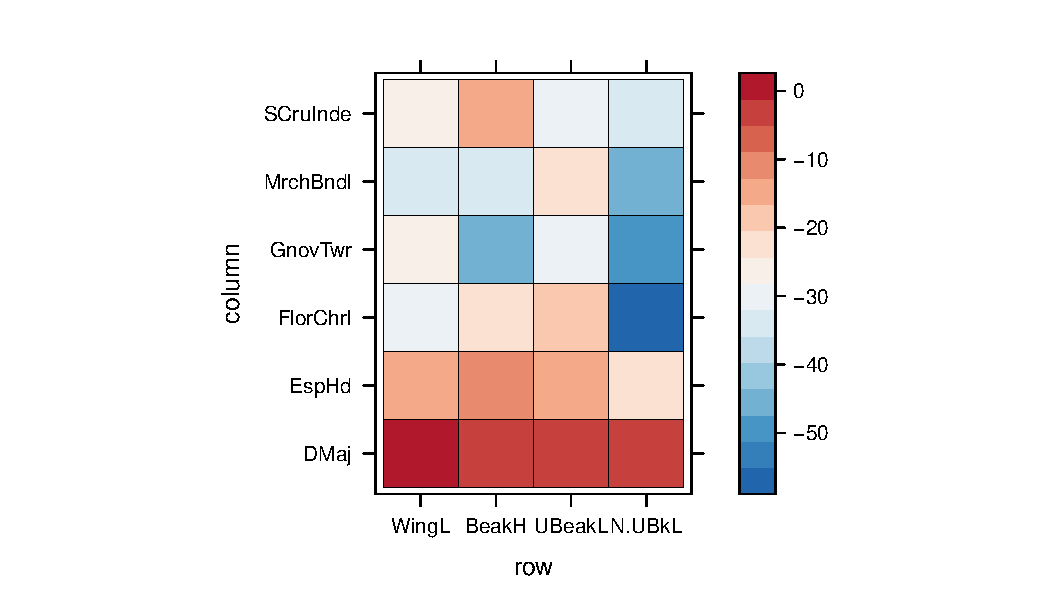
\includegraphics[width=\maxwidth]{figure/unnamed-chunk-641} 
\begin{kframe}\begin{alltt}
=======


{\ttfamily\noindent\bfseries\color{errorcolor}{\#\# Error: erreur d'évaluation de l'argument 'x' lors de la sélection d'une méthode pour la fonction 'levelplot' : Erreur dans t(ses(res.finch\$Tstats\$T\_IP.IC, res.finch\$Tstats\$T\_IP.IC\_nm)\$ses) : \\\#\#\ \  erreur d'évaluation de l'argument 'x' lors de la sélection d'une méthode pour la fonction 't' : Erreur dans is.vector(obs) : objet 'res.finch' introuvable\\\#\# Calls: ses -> is.vector}}\begin{alltt}
>>>>>>> 5f89dfbb4bbfa61805f8e116f94cee418c14cfee
\hlkwd{levelplot}\hlstd{(}\hlkwd{cbind}\hlstd{(}\hlkwd{t}\hlstd{(}\hlkwd{ses}\hlstd{(res.finch}\hlopt{$}\hlstd{Tstats}\hlopt{$}\hlstd{T_IP.IC, res.finch}\hlopt{$}\hlstd{Tstats}\hlopt{$}\hlstd{T_IP.IC_nm)}\hlopt{$}\hlstd{ses),}
        \hlkwd{t}\hlstd{(}\hlkwd{ses}\hlstd{(res.finch}\hlopt{$}\hlstd{Tstats}\hlopt{$}\hlstd{T_IC.IR, res.finch}\hlopt{$}\hlstd{Tstats}\hlopt{$}\hlstd{T_IP.IC_nm)}\hlopt{$}\hlstd{ses),}
        \hlkwd{t}\hlstd{(}\hlkwd{ses}\hlstd{(res.finch}\hlopt{$}\hlstd{Tstats}\hlopt{$}\hlstd{T_PC.PR, res.finch}\hlopt{$}\hlstd{Tstats}\hlopt{$}\hlstd{T_IP.IC_nm)}\hlopt{$}\hlstd{ses))}
     \hlstd{,} \hlkwc{colorkey} \hlstd{= my.ckey,} \hlkwc{par.settings} \hlstd{= my.theme,}\hlkwc{border} \hlstd{=} \hlstr{"black"}\hlstd{)}
\end{alltt}
<<<<<<< HEAD
\end{kframe}
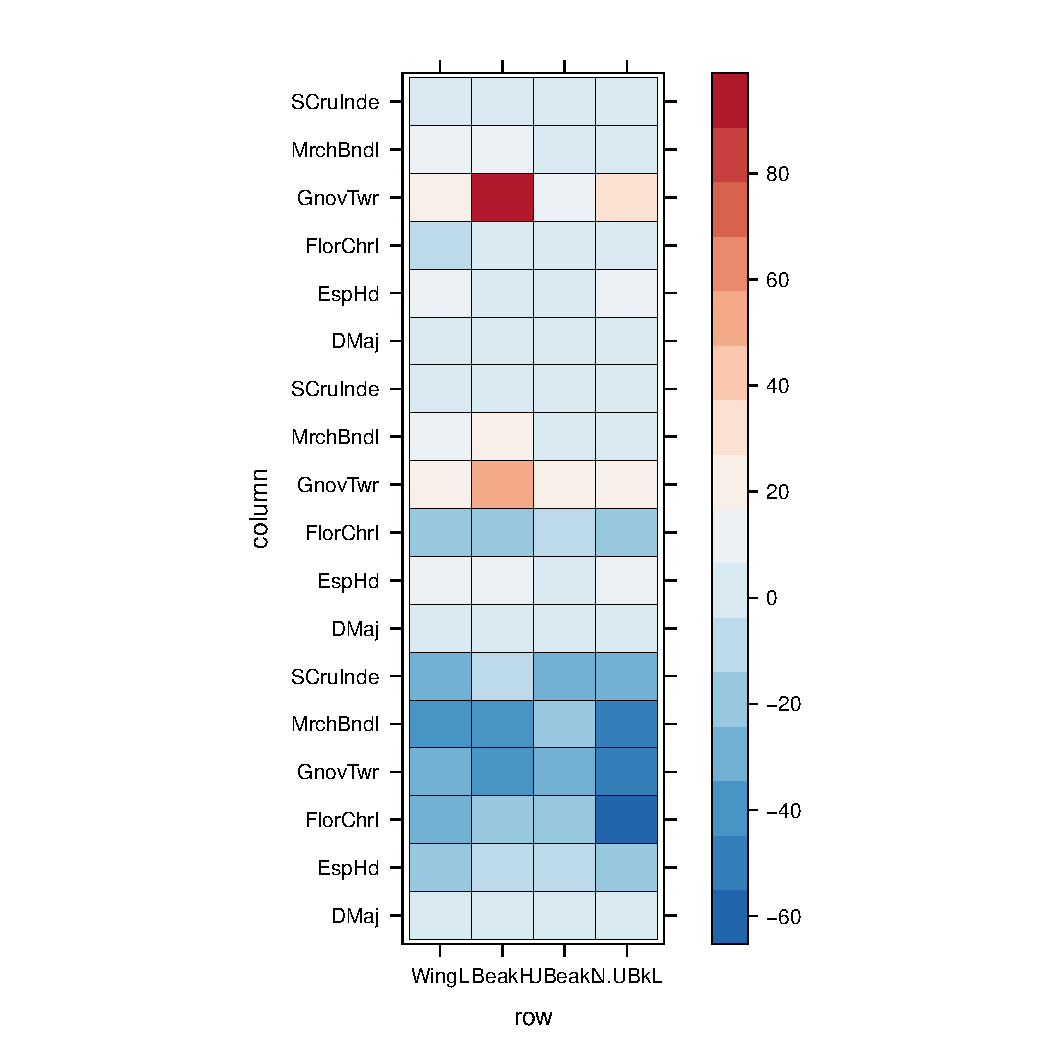
\includegraphics[width=\maxwidth]{figure/unnamed-chunk-642} 
=======
>>>>>>> 5f89dfbb4bbfa61805f8e116f94cee418c14cfee


{\ttfamily\noindent\bfseries\color{errorcolor}{\#\# Error: erreur d'évaluation de l'argument 'x' lors de la sélection d'une méthode pour la fonction 'levelplot' : Erreur dans t(ses(res.finch\$Tstats\$T\_IP.IC, res.finch\$Tstats\$T\_IP.IC\_nm)\$ses) : \\\#\#\ \  erreur d'évaluation de l'argument 'x' lors de la sélection d'une méthode pour la fonction 't' : Erreur dans is.vector(obs) : objet 'res.finch' introuvable\\\#\# Calls: ses -> is.vector\\\#\# Calls: cbind -> t}}\end{kframe}
\end{knitrout}

Another example using \texttt{ses.listofindex}. The first plot represent "ses" values and the second one the result of a test with H0: observed index value are greater than what we can expect using the null model (alpha = 2.5\%).

\begin{knitrout}
\definecolor{shadecolor}{rgb}{0.969, 0.969, 0.969}\color{fgcolor}\begin{kframe}
\begin{alltt}
\hlstd{ses.list}\hlkwb{<-}\hlkwd{ses.listofindex}\hlstd{(i.l1)}
\end{alltt}


{\ttfamily\noindent\bfseries\color{errorcolor}{\#\# Error: objet 'i.l1' introuvable}}\begin{alltt}
\hlkwd{levelplot}\hlstd{(}\hlkwd{t}\hlstd{(}\hlkwd{rbind}\hlstd{(ses.list[[}\hlnum{1}\hlstd{]]}\hlopt{$}\hlstd{ses, ses.list[[}\hlnum{2}\hlstd{]]}\hlopt{$}\hlstd{ses,}
         \hlstd{ses.list[[}\hlnum{3}\hlstd{]]}\hlopt{$}\hlstd{ses, ses.list[[}\hlnum{4}\hlstd{]]}\hlopt{$}\hlstd{ses)),}
     \hlkwc{colorkey} \hlstd{= my.ckey,} \hlkwc{par.settings} \hlstd{= my.theme,}\hlkwc{border} \hlstd{=} \hlstr{"black"}\hlstd{)}
\end{alltt}
<<<<<<< HEAD
\end{kframe}
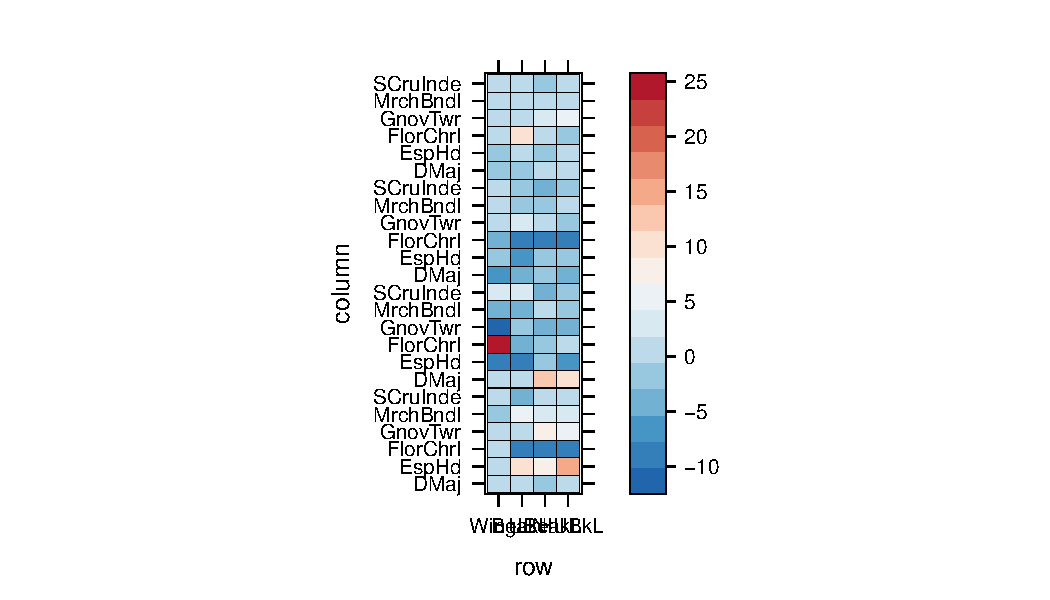
\includegraphics[width=\maxwidth]{figure/unnamed-chunk-651} 
\begin{kframe}\begin{alltt}
=======


{\ttfamily\noindent\bfseries\color{errorcolor}{\#\# Error: erreur d'évaluation de l'argument 'x' lors de la sélection d'une méthode pour la fonction 'levelplot' : Erreur dans t(rbind(ses.list[[1]]\$ses, ses.list[[2]]\$ses, ses.list[[3]]\$ses,\ \ : \\\#\#\ \  erreur d'évaluation de l'argument 'x' lors de la sélection d'une méthode pour la fonction 't' : Erreur dans rbind(ses.list[[1]]\$ses, ses.list[[2]]\$ses, ses.list[[3]]\$ses,\ \ : \\\#\#\ \  objet 'ses.list' introuvable}}\begin{alltt}
>>>>>>> 5f89dfbb4bbfa61805f8e116f94cee418c14cfee
\hlkwd{levelplot}\hlstd{(}\hlkwd{t}\hlstd{(}\hlkwd{rbind}\hlstd{(ses.list[[}\hlnum{1}\hlstd{]]}\hlopt{$}\hlstd{ses}\hlopt{>}\hlstd{ses.list[[}\hlnum{1}\hlstd{]]}\hlopt{$}\hlstd{ses.sup,}
         \hlstd{ses.list[[}\hlnum{2}\hlstd{]]}\hlopt{$}\hlstd{ses}\hlopt{>}\hlstd{ses.list[[}\hlnum{2}\hlstd{]]}\hlopt{$}\hlstd{ses.sup,}
         \hlstd{ses.list[[}\hlnum{3}\hlstd{]]}\hlopt{$}\hlstd{ses}\hlopt{>}\hlstd{ses.list[[}\hlnum{3}\hlstd{]]}\hlopt{$}\hlstd{ses.sup,}
         \hlstd{ses.list[[}\hlnum{4}\hlstd{]]}\hlopt{$}\hlstd{ses}\hlopt{>}\hlstd{ses.list[[}\hlnum{4}\hlstd{]]}\hlopt{$}\hlstd{ses.sup)),}
     \hlkwc{colorkey} \hlstd{= my.ckey,} \hlkwc{par.settings} \hlstd{= my.theme,}\hlkwc{border} \hlstd{=} \hlstr{"black"}\hlstd{)}
\end{alltt}
<<<<<<< HEAD
\end{kframe}
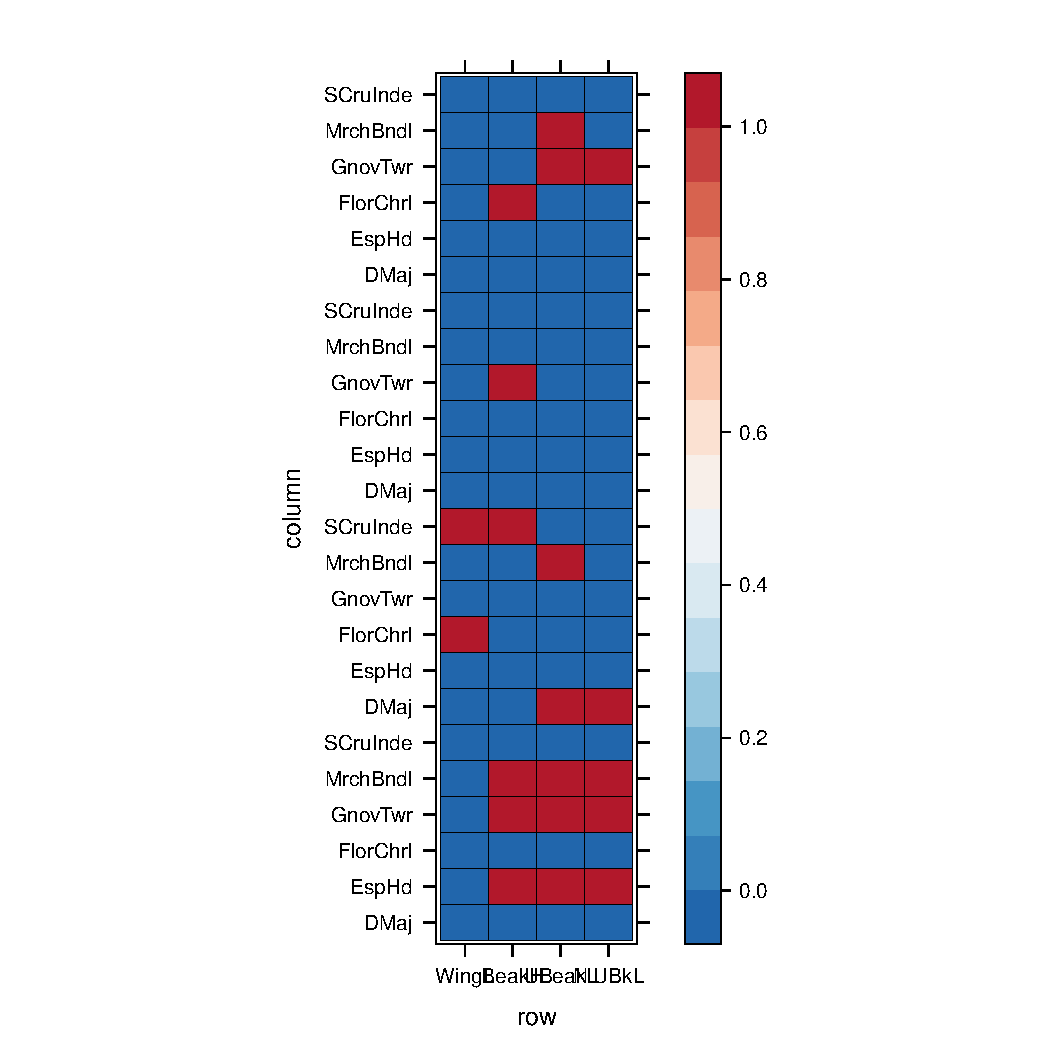
\includegraphics[width=\maxwidth]{figure/unnamed-chunk-652} 
=======
>>>>>>> 5f89dfbb4bbfa61805f8e116f94cee418c14cfee


{\ttfamily\noindent\bfseries\color{errorcolor}{\#\# Error: erreur d'évaluation de l'argument 'x' lors de la sélection d'une méthode pour la fonction 'levelplot' : Erreur dans t(rbind(ses.list[[1]]\$ses > ses.list[[1]]\$ses.sup, ses.list[[2]]\$ses >\ \ : \\\#\#\ \  erreur d'évaluation de l'argument 'x' lors de la sélection d'une méthode pour la fonction 't' : Erreur dans rbind(ses.list[[1]]\$ses > ses.list[[1]]\$ses.sup, ses.list[[2]]\$ses >\ \ : \\\#\#\ \  objet 'ses.list' introuvable}}\end{kframe}
\end{knitrout}

Compare metrics calculate on individual against metrics calculate after populationnal meaning
\begin{knitrout}
\definecolor{shadecolor}{rgb}{0.969, 0.969, 0.969}\color{fgcolor}\begin{kframe}
\begin{alltt}
\hlstd{ses.ind}\hlkwb{<-}\hlkwd{t}\hlstd{(}\hlkwd{rbind}\hlstd{(ses.list[[}\hlnum{1}\hlstd{]]}\hlopt{$}\hlstd{ses,}
      \hlstd{ses.list[[}\hlnum{2}\hlstd{]]}\hlopt{$}\hlstd{ses,}
      \hlstd{ses.list[[}\hlnum{3}\hlstd{]]}\hlopt{$}\hlstd{ses,}
      \hlstd{ses.list[[}\hlnum{4}\hlstd{]]}\hlopt{$}\hlstd{ses))}
\end{alltt}


{\ttfamily\noindent\bfseries\color{errorcolor}{\#\# Error: erreur d'évaluation de l'argument 'x' lors de la sélection d'une méthode pour la fonction 't' : Erreur dans rbind(ses.list[[1]]\$ses, ses.list[[2]]\$ses, ses.list[[3]]\$ses,\ \ : \\\#\#\ \  objet 'ses.list' introuvable}}\begin{alltt}
\hlstd{ses.sp}\hlkwb{<-}\hlkwd{t}\hlstd{(}\hlkwd{rbind}\hlstd{(ses.list[[}\hlnum{5}\hlstd{]]}\hlopt{$}\hlstd{ses,}
     \hlstd{ses.list[[}\hlnum{6}\hlstd{]]}\hlopt{$}\hlstd{ses,}
     \hlstd{ses.list[[}\hlnum{7}\hlstd{]]}\hlopt{$}\hlstd{ses,}
     \hlstd{ses.list[[}\hlnum{8}\hlstd{]]}\hlopt{$}\hlstd{ses))}
\end{alltt}


{\ttfamily\noindent\bfseries\color{errorcolor}{\#\# Error: erreur d'évaluation de l'argument 'x' lors de la sélection d'une méthode pour la fonction 't' : Erreur dans rbind(ses.list[[5]]\$ses, ses.list[[6]]\$ses, ses.list[[7]]\$ses,\ \ : \\\#\#\ \  objet 'ses.list' introuvable}}\begin{alltt}
\hlkwd{levelplot}\hlstd{(ses.ind,} \hlkwc{colorkey} \hlstd{= my.ckey,}
     \hlkwc{par.settings} \hlstd{= my.theme,}\hlkwc{border} \hlstd{=} \hlstr{"black"}\hlstd{)}
\end{alltt}
<<<<<<< HEAD
\end{kframe}
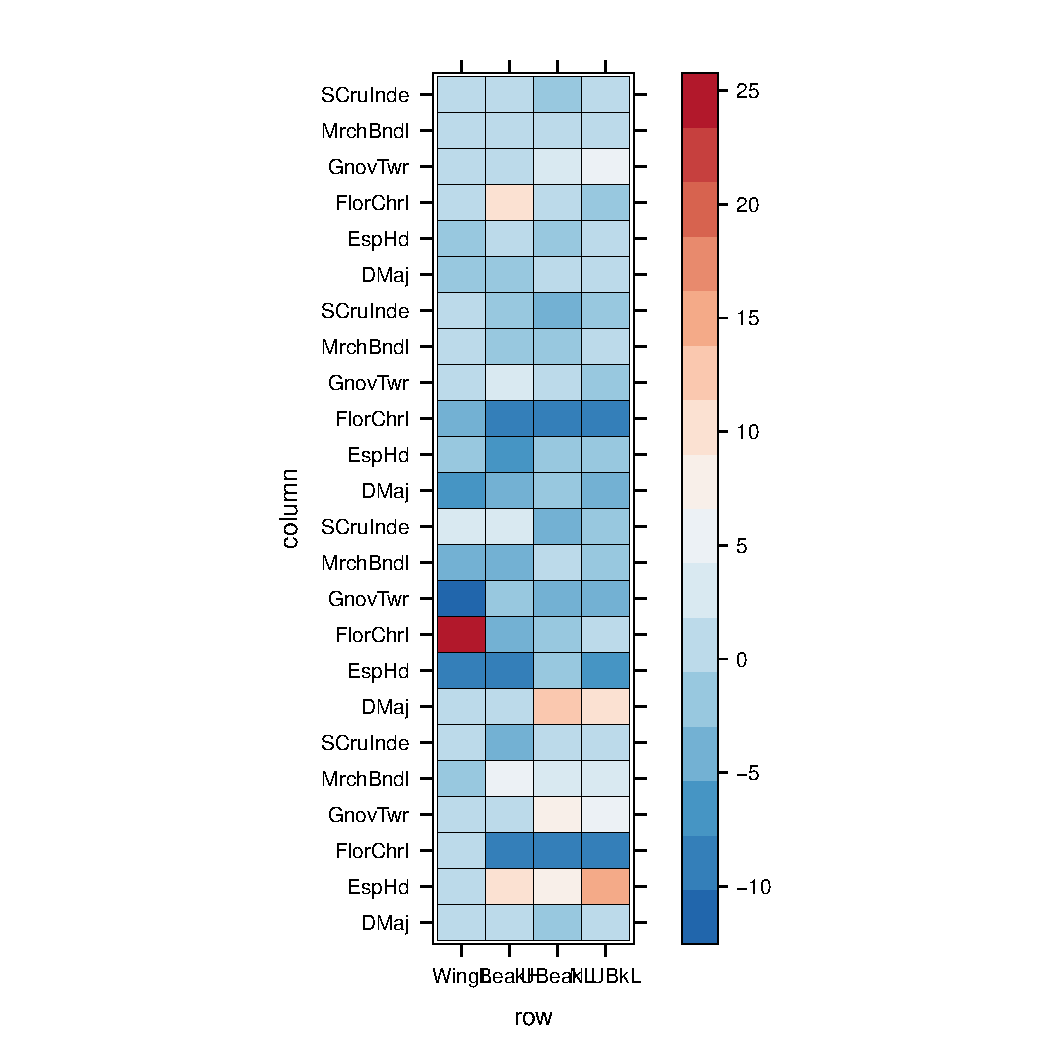
\includegraphics[width=\maxwidth]{figure/unnamed-chunk-661} 
\begin{kframe}\begin{alltt}
\hlkwd{levelplot}\hlstd{(ses.sp,} \hlkwc{colorkey} \hlstd{= my.ckey,}
     \hlkwc{par.settings} \hlstd{= my.theme,}\hlkwc{border} \hlstd{=} \hlstr{"black"}\hlstd{)}
\end{alltt}
\end{kframe}
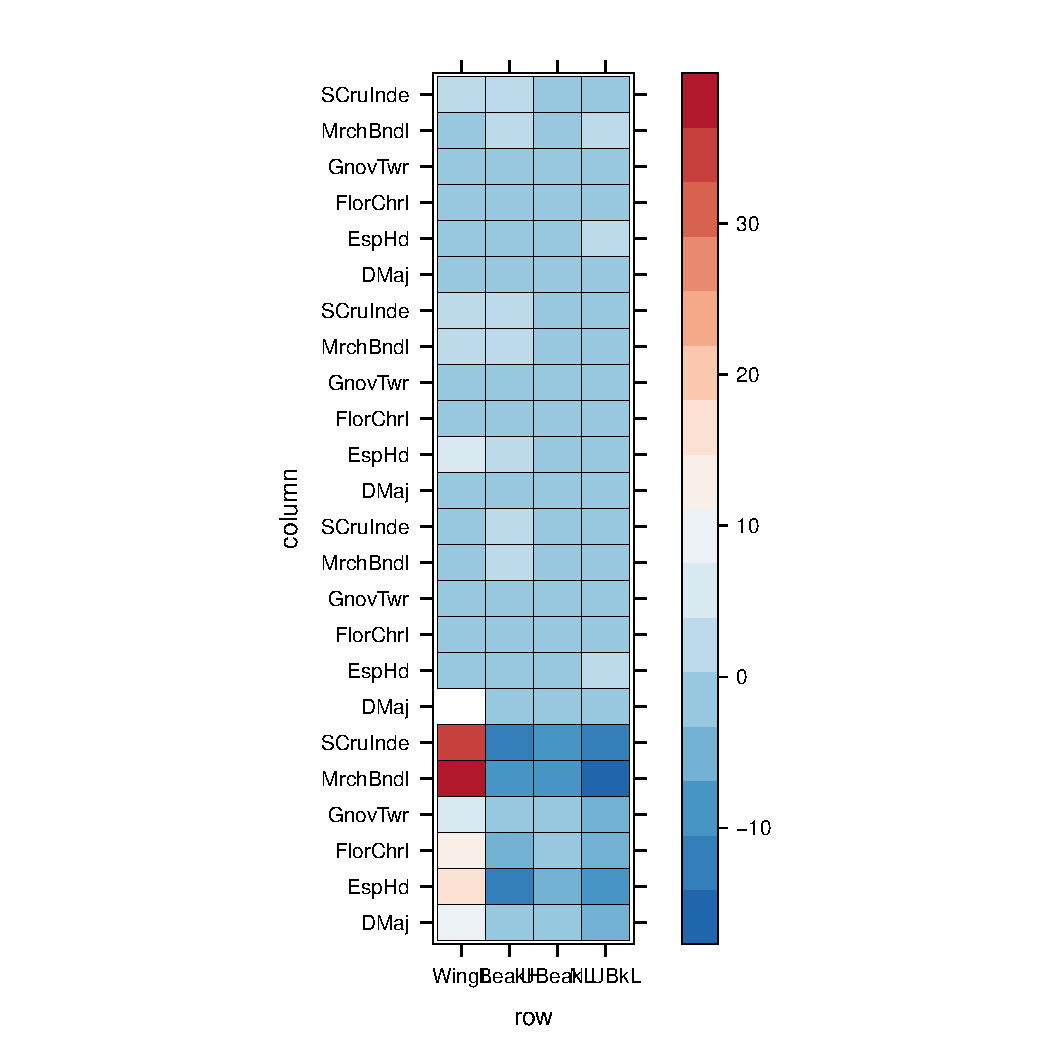
\includegraphics[width=\maxwidth]{figure/unnamed-chunk-662} 
=======


{\ttfamily\noindent\bfseries\color{errorcolor}{\#\# Error: erreur d'évaluation de l'argument 'x' lors de la sélection d'une méthode pour la fonction 'levelplot' : Erreur : objet 'ses.ind' introuvable}}\begin{alltt}
\hlkwd{levelplot}\hlstd{(ses.sp,} \hlkwc{colorkey} \hlstd{= my.ckey,}
     \hlkwc{par.settings} \hlstd{= my.theme,}\hlkwc{border} \hlstd{=} \hlstr{"black"}\hlstd{)}
\end{alltt}
>>>>>>> 5f89dfbb4bbfa61805f8e116f94cee418c14cfee


{\ttfamily\noindent\bfseries\color{errorcolor}{\#\# Error: erreur d'évaluation de l'argument 'x' lors de la sélection d'une méthode pour la fonction 'levelplot' : Erreur : objet 'ses.sp' introuvable}}\end{kframe}
\end{knitrout}

\section{Multivariate analysis of metrics}
To finish, we can do a multivariate analysis of the metrics obtain during this tutorial using the package \texttt{ade4}. Analysis dudi 1 puts together all traits by meaning the SES values for each metrics in each sites whereas analysis dudi 2 analyses all combination of traits / sites / metrics.

\begin{knitrout}
\definecolor{shadecolor}{rgb}{0.969, 0.969, 0.969}\color{fgcolor}\begin{kframe}
\begin{alltt}
\hlkwd{library}\hlstd{(ade4)}

 \hlstd{matfordudi}\hlkwb{<-}\hlkwd{matrix}\hlstd{(}\hlkwc{nrow} \hlstd{=} \hlkwd{length}\hlstd{(}\hlkwd{colMeans}\hlstd{(ses.list[[}\hlnum{1}\hlstd{]]}\hlopt{$}\hlstd{ses)),} \hlkwc{ncol} \hlstd{=} \hlkwd{length}\hlstd{(}\hlkwd{names}\hlstd{(ses.list)))}
\end{alltt}


{\ttfamily\noindent\bfseries\color{errorcolor}{\#\# Error: objet 'ses.list' introuvable}}\begin{alltt}
 \hlkwa{for}\hlstd{(i} \hlkwa{in} \hlnum{1}\hlopt{:} \hlkwd{length}\hlstd{(}\hlkwd{names}\hlstd{(ses.list)))\{}
  \hlstd{matfordudi[,i]}\hlkwb{<-}\hlkwd{colMeans}\hlstd{(ses.list[[i]]}\hlopt{$}\hlstd{ses)}
 \hlstd{\}}
\end{alltt}


{\ttfamily\noindent\bfseries\color{errorcolor}{\#\# Error: objet 'ses.list' introuvable}}\begin{alltt}
 \hlkwd{colnames}\hlstd{(matfordudi)}\hlkwb{<-}\hlkwd{names}\hlstd{(ses.list)}
\end{alltt}


{\ttfamily\noindent\bfseries\color{errorcolor}{\#\# Error: objet 'ses.list' introuvable}}\begin{alltt}
 \hlkwd{rownames}\hlstd{(matfordudi)}\hlkwb{<-}\hlkwd{colnames}\hlstd{(traits.finch)}
\end{alltt}


{\ttfamily\noindent\bfseries\color{errorcolor}{\#\# Error: objet 'matfordudi' introuvable}}\begin{alltt}
 \hlstd{matfordudi2}\hlkwb{<-}\hlkwd{matrix}\hlstd{(}\hlkwc{nrow} \hlstd{=} \hlkwd{length}\hlstd{(}\hlkwd{as.vector}\hlstd{(ses.list[[}\hlnum{1}\hlstd{]]}\hlopt{$}\hlstd{ses)),} \hlkwc{ncol} \hlstd{=} \hlkwd{length}\hlstd{(}\hlkwd{names}\hlstd{(ses.list)))}
\end{alltt}


{\ttfamily\noindent\bfseries\color{errorcolor}{\#\# Error: erreur d'évaluation de l'argument 'x' lors de la sélection d'une méthode pour la fonction 'as.vector' : Erreur : objet 'ses.list' introuvable}}\begin{alltt}
 \hlkwa{for}\hlstd{(i} \hlkwa{in} \hlnum{1}\hlopt{:} \hlkwd{length}\hlstd{(}\hlkwd{names}\hlstd{(ses.list)))\{}
  \hlstd{matfordudi2[,i]}\hlkwb{<-}\hlkwd{as.vector}\hlstd{(ses.list[[i]]}\hlopt{$}\hlstd{ses)}
 \hlstd{\}}
\end{alltt}


{\ttfamily\noindent\bfseries\color{errorcolor}{\#\# Error: objet 'ses.list' introuvable}}\begin{alltt}
 \hlkwd{colnames}\hlstd{(matfordudi2)}\hlkwb{<-}\hlkwd{names}\hlstd{(ses.list)}
\end{alltt}


{\ttfamily\noindent\bfseries\color{errorcolor}{\#\# Error: objet 'ses.list' introuvable}}\end{kframe}
\end{knitrout}

\begin{knitrout}
\definecolor{shadecolor}{rgb}{0.969, 0.969, 0.969}\color{fgcolor}\begin{kframe}
\begin{alltt}
\hlcom{#Use mice for the purpose of this example}
\hlstd{matfordudi}\hlkwb{<-}\hlkwd{complete}\hlstd{(}\hlkwd{mice}\hlstd{(matfordudi))}
\end{alltt}


{\ttfamily\noindent\bfseries\color{errorcolor}{\#\# Error: objet 'matfordudi' introuvable}}\begin{alltt}
\hlstd{matfordudi2}\hlkwb{<-}\hlkwd{complete}\hlstd{(}\hlkwd{mice}\hlstd{(matfordudi2))}
\end{alltt}


{\ttfamily\noindent\bfseries\color{errorcolor}{\#\# Error: objet 'matfordudi2' introuvable}}\end{kframe}
\end{knitrout}


\begin{knitrout}
\definecolor{shadecolor}{rgb}{0.969, 0.969, 0.969}\color{fgcolor}\begin{kframe}
\begin{alltt}
\hlstd{res.dudi}\hlkwb{<-}\hlkwd{dudi.pca}\hlstd{(}\hlkwd{t}\hlstd{(matfordudi),} \hlkwc{scan} \hlstd{= F,} \hlkwc{nf} \hlstd{=} \hlnum{2}\hlstd{)}
\end{alltt}


{\ttfamily\noindent\bfseries\color{errorcolor}{\#\# Error: erreur d'évaluation de l'argument 'x' lors de la sélection d'une méthode pour la fonction 't' : Erreur : objet 'matfordudi' introuvable}}\begin{alltt}
\hlkwd{s.corcircle}\hlstd{(res.dudi}\hlopt{$}\hlstd{co)}
\end{alltt}


{\ttfamily\noindent\bfseries\color{errorcolor}{\#\# Error: objet 'res.dudi' introuvable}}\begin{alltt}
\hlkwd{s.label}\hlstd{(res.dudi}\hlopt{$}\hlstd{li,} \hlkwc{add.plot} \hlstd{= T,} \hlkwc{clabel} \hlstd{=} \hlnum{0}\hlstd{,} \hlkwc{pch} \hlstd{=} \hlnum{16}\hlstd{)}
\end{alltt}


{\ttfamily\noindent\bfseries\color{errorcolor}{\#\# Error: objet 'res.dudi' introuvable}}\begin{alltt}
\hlkwd{s.label}\hlstd{(res.dudi}\hlopt{$}\hlstd{li}\hlopt{+}\hlnum{0.05}\hlstd{,} \hlkwc{add.plot} \hlstd{= T,} \hlkwc{boxes} \hlstd{= F)}
\end{alltt}
<<<<<<< HEAD
\end{kframe}
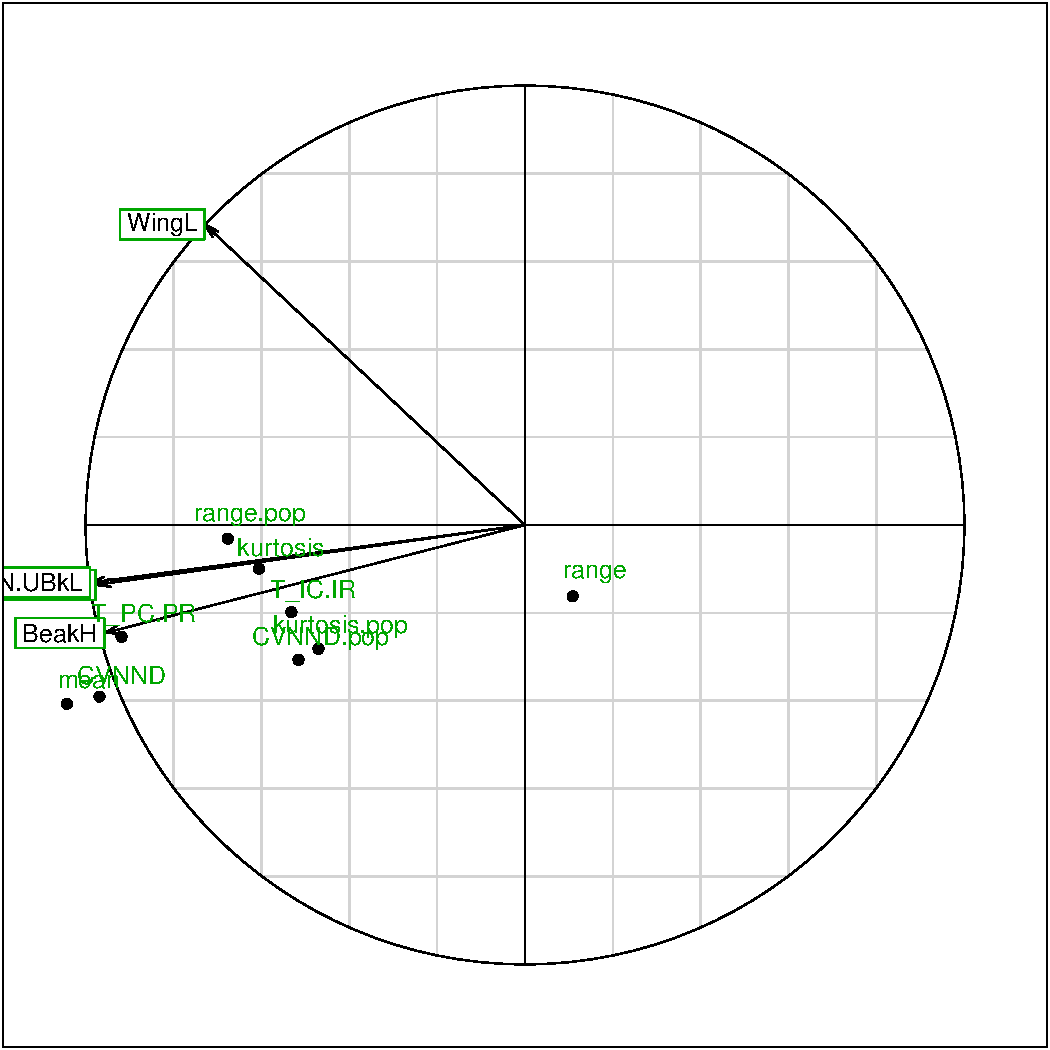
\includegraphics[width=\maxwidth]{figure/unnamed-chunk-691} 
\begin{kframe}\begin{alltt}
=======


{\ttfamily\noindent\bfseries\color{errorcolor}{\#\# Error: objet 'res.dudi' introuvable}}\begin{alltt}
>>>>>>> 5f89dfbb4bbfa61805f8e116f94cee418c14cfee
\hlstd{res.dudi2}\hlkwb{<-}\hlkwd{dudi.pca}\hlstd{(matfordudi2,} \hlkwc{scan} \hlstd{= F,} \hlkwc{nf} \hlstd{=} \hlnum{2}\hlstd{)}
\end{alltt}


{\ttfamily\noindent\bfseries\color{errorcolor}{\#\# Error: objet 'matfordudi2' introuvable}}\begin{alltt}
\hlkwd{scatter}\hlstd{(res.dudi2)}
\end{alltt}
<<<<<<< HEAD
\end{kframe}
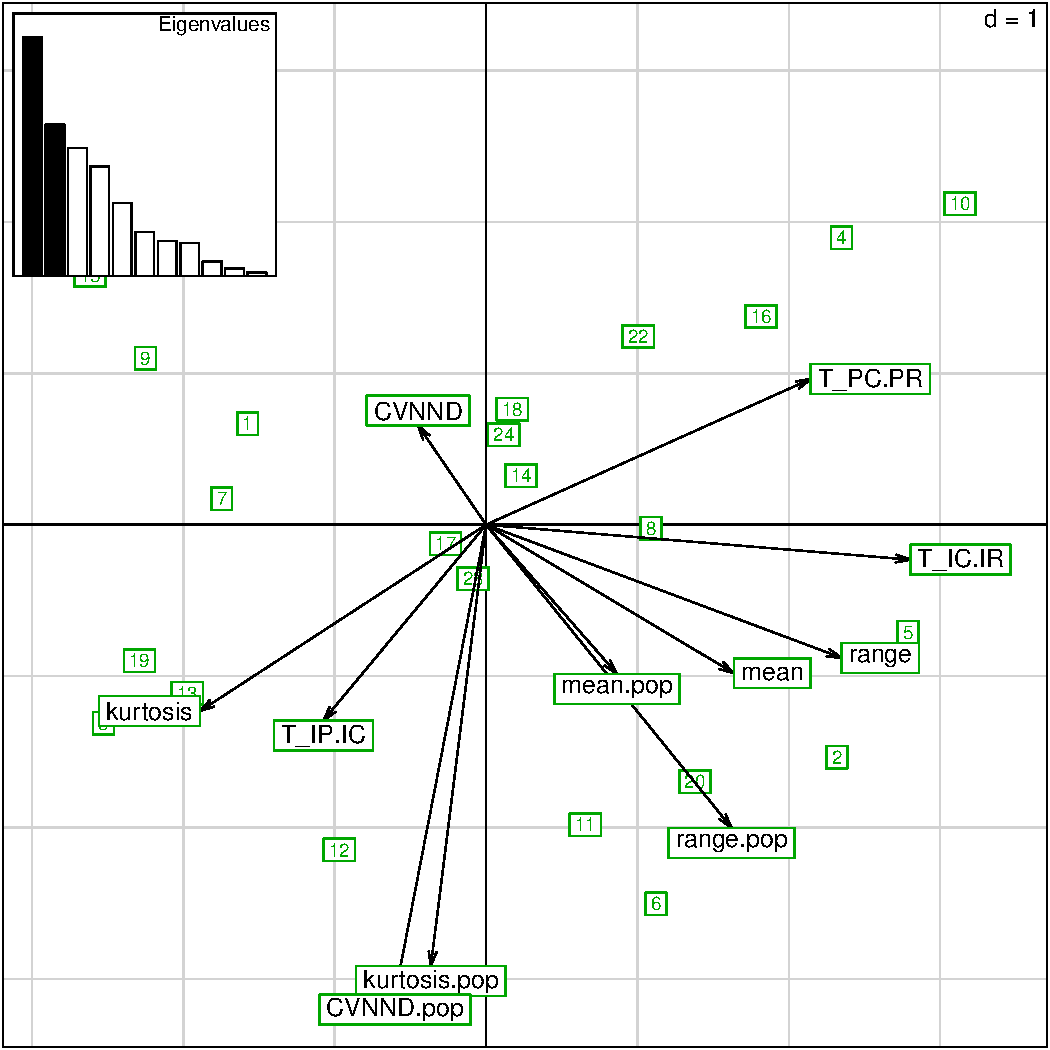
\includegraphics[width=\maxwidth]{figure/unnamed-chunk-692} 
\begin{kframe}\begin{alltt}
\hlkwd{s.corcircle}\hlstd{(res.dudi2}\hlopt{$}\hlstd{co)}
\end{alltt}
\end{kframe}
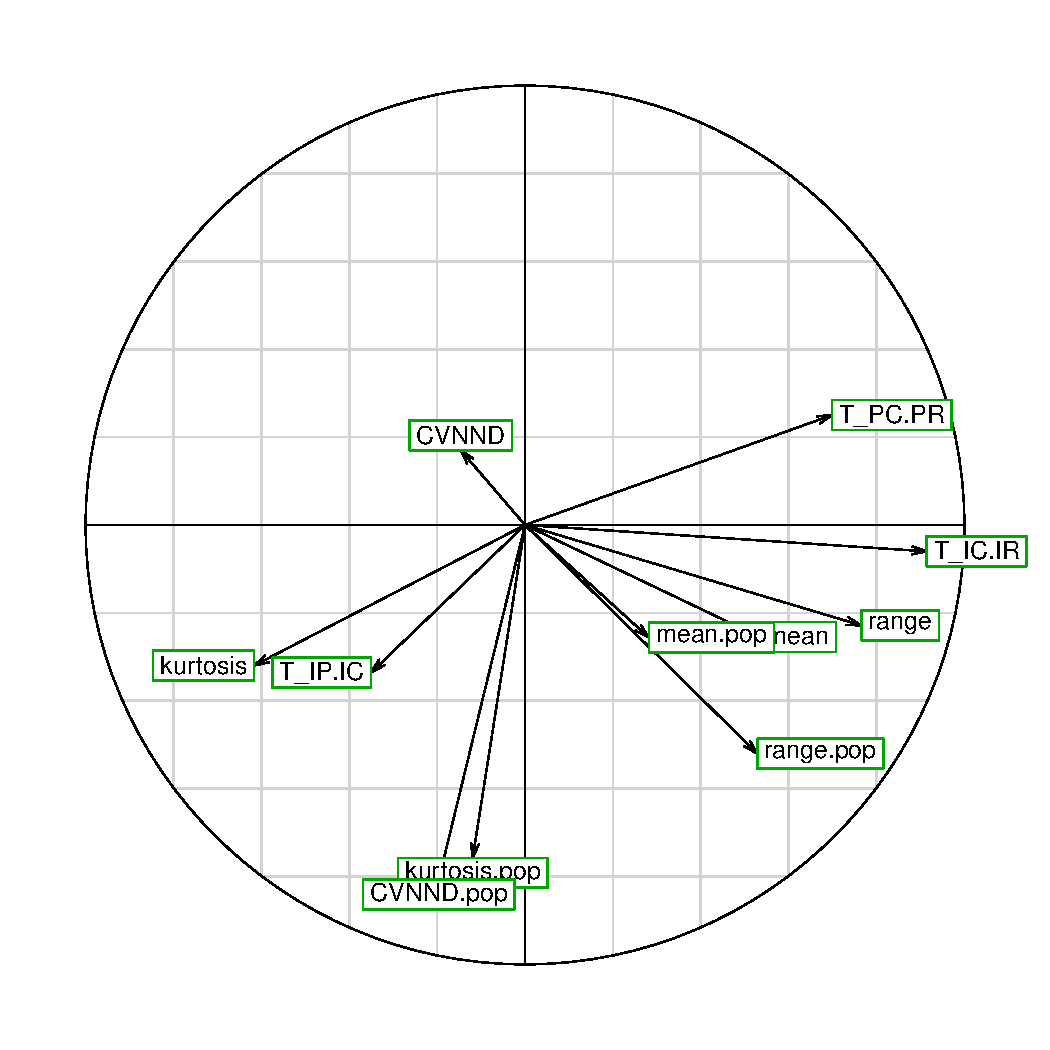
\includegraphics[width=\maxwidth]{figure/unnamed-chunk-693} 
\begin{kframe}\begin{alltt}
\hlkwd{s.class}\hlstd{(res.dudi2}\hlopt{$}\hlstd{li,} \hlkwd{as.factor}\hlstd{(}\hlkwd{c}\hlstd{(}\hlkwd{rep}\hlstd{(}\hlstr{"WingL"}\hlstd{,}\hlnum{6}\hlstd{),} \hlkwd{rep}\hlstd{(}\hlstr{"BeakH"}\hlstd{,}\hlnum{6}\hlstd{),} \hlkwd{rep}\hlstd{(}\hlstr{"UBeakL"}\hlstd{,}\hlnum{6}\hlstd{),} \hlkwd{rep}\hlstd{(}\hlstr{"N.UBkL"}\hlstd{,}\hlnum{6}\hlstd{))),} \hlkwc{col} \hlstd{=} \hlkwd{funky}\hlstd{(}\hlnum{4}\hlstd{))}
\end{alltt}
\end{kframe}
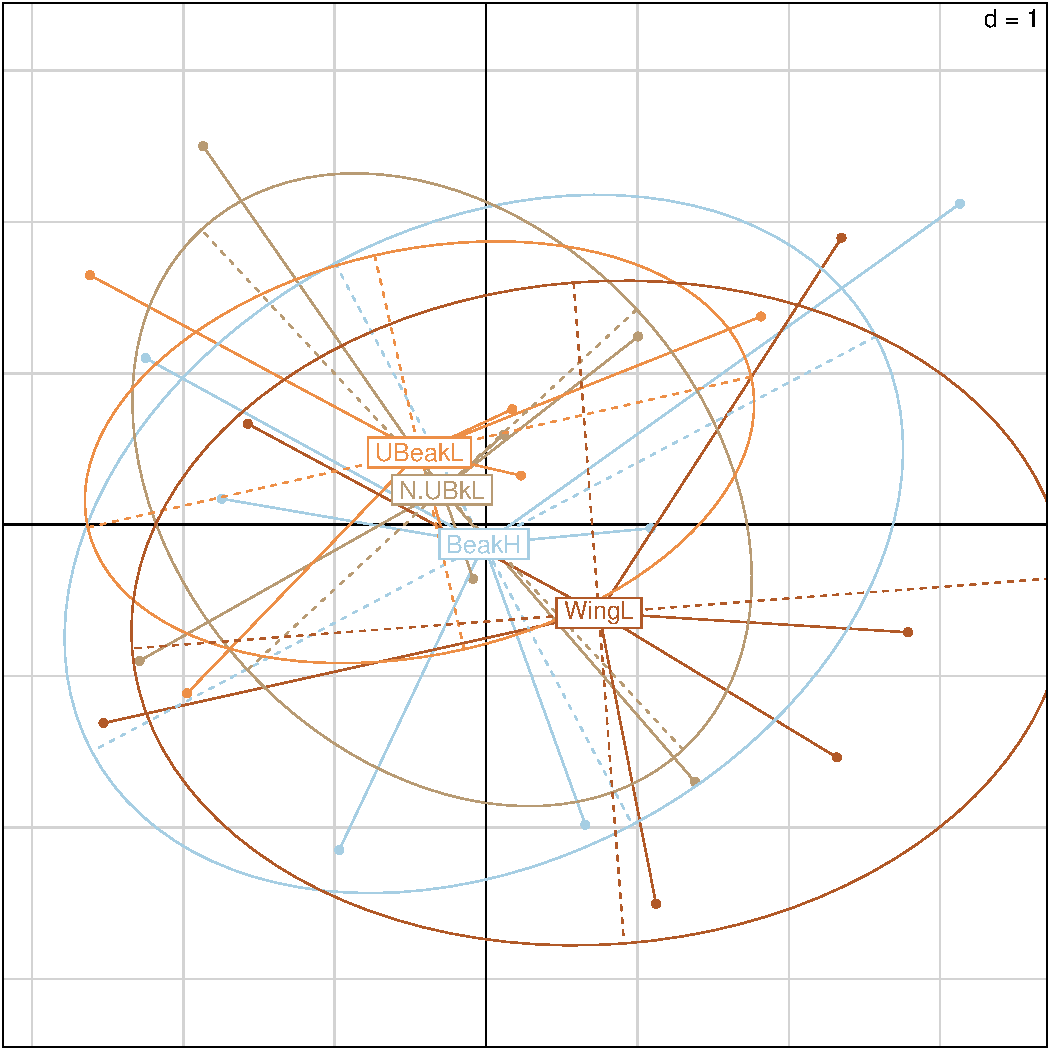
\includegraphics[width=\maxwidth]{figure/unnamed-chunk-694} 
\begin{kframe}\begin{alltt}
\hlkwd{s.class}\hlstd{(res.dudi2}\hlopt{$}\hlstd{li,} \hlkwd{as.factor}\hlstd{(}\hlkwd{rep}\hlstd{(}\hlkwd{c}\hlstd{(}\hlstr{"DMaj"}\hlstd{,}\hlstr{"EspHd"}\hlstd{,}\hlstr{"FlorChrl"}\hlstd{,}\hlstr{"GnovTwr"}\hlstd{,}\hlstr{"MrchBndl"}\hlstd{,}\hlstr{"SCruInde"}\hlstd{),}\hlnum{4} \hlstd{)),} \hlkwc{col} \hlstd{=} \hlkwd{funky}\hlstd{(}\hlnum{6}\hlstd{))}
\end{alltt}
\end{kframe}
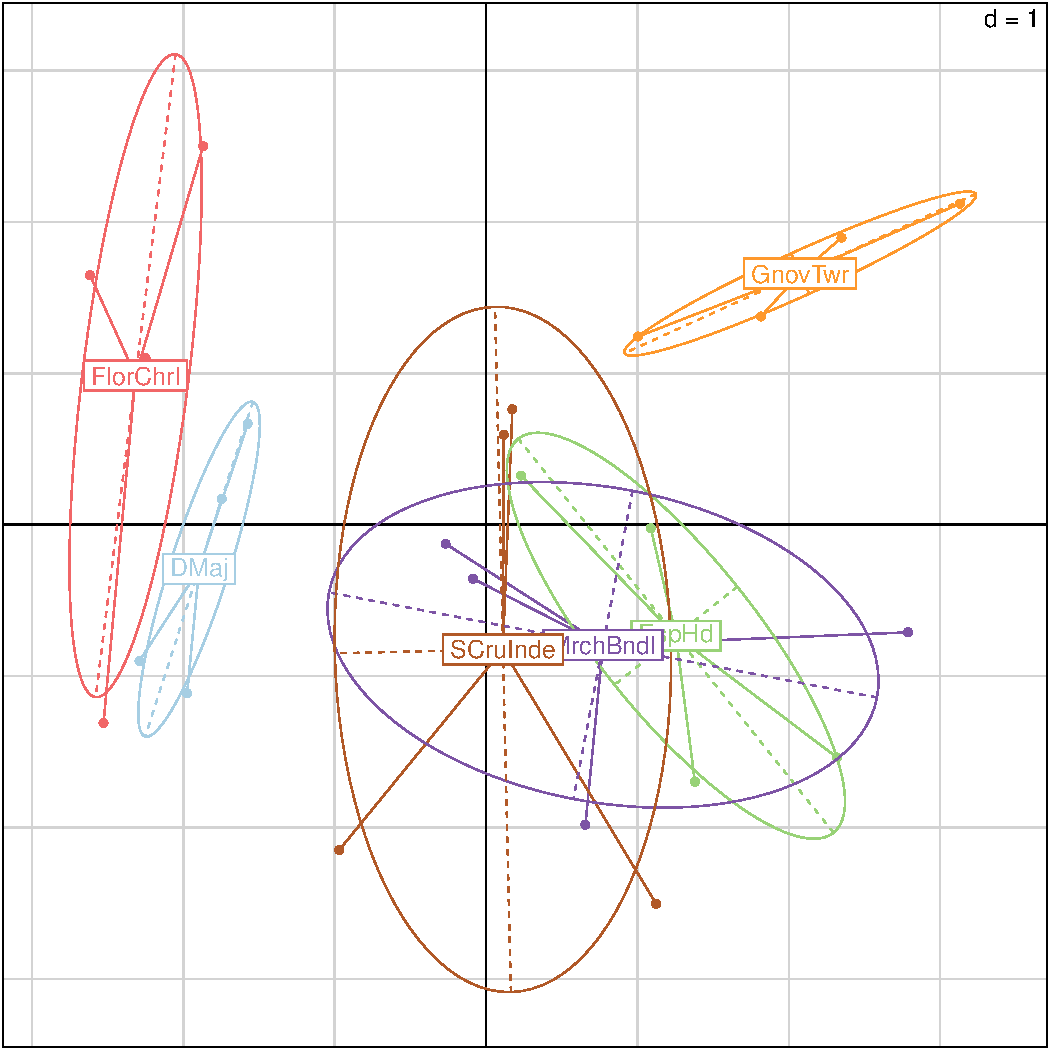
\includegraphics[width=\maxwidth]{figure/unnamed-chunk-695} 
=======


{\ttfamily\noindent\bfseries\color{errorcolor}{\#\# Error: objet 'res.dudi2' introuvable}}\begin{alltt}
\hlkwd{s.corcircle}\hlstd{(res.dudi2}\hlopt{$}\hlstd{co)}
\end{alltt}


{\ttfamily\noindent\bfseries\color{errorcolor}{\#\# Error: objet 'res.dudi2' introuvable}}\begin{alltt}
\hlkwd{s.class}\hlstd{(res.dudi2}\hlopt{$}\hlstd{li,} \hlkwd{as.factor}\hlstd{(}\hlkwd{c}\hlstd{(}\hlkwd{rep}\hlstd{(}\hlstr{"WingL"}\hlstd{,}\hlnum{6}\hlstd{),} \hlkwd{rep}\hlstd{(}\hlstr{"BeakH"}\hlstd{,}\hlnum{6}\hlstd{),} \hlkwd{rep}\hlstd{(}\hlstr{"UBeakL"}\hlstd{,}\hlnum{6}\hlstd{),} \hlkwd{rep}\hlstd{(}\hlstr{"N.UBkL"}\hlstd{,}\hlnum{6}\hlstd{))),} \hlkwc{col} \hlstd{=} \hlkwd{funky}\hlstd{(}\hlnum{4}\hlstd{))}
\end{alltt}


{\ttfamily\noindent\bfseries\color{errorcolor}{\#\# Error: objet 'res.dudi2' introuvable}}\begin{alltt}
\hlkwd{s.class}\hlstd{(res.dudi2}\hlopt{$}\hlstd{li,} \hlkwd{as.factor}\hlstd{(}\hlkwd{rep}\hlstd{(}\hlkwd{c}\hlstd{(}\hlstr{"DMaj"}\hlstd{,}\hlstr{"EspHd"}\hlstd{,}\hlstr{"FlorChrl"}\hlstd{,}\hlstr{"GnovTwr"}\hlstd{,}\hlstr{"MrchBndl"}\hlstd{,}\hlstr{"SCruInde"}\hlstd{),}\hlnum{4} \hlstd{)),} \hlkwc{col} \hlstd{=} \hlkwd{funky}\hlstd{(}\hlnum{6}\hlstd{))}
\end{alltt}
>>>>>>> 5f89dfbb4bbfa61805f8e116f94cee418c14cfee


{\ttfamily\noindent\bfseries\color{errorcolor}{\#\# Error: objet 'res.dudi2' introuvable}}\end{kframe}
\end{knitrout}

\section*{Conclusion}
\addcontentsline{toc}{subsection}{Conclusion}
This is the end of the tutorial. The up to date version of this tutorial is available \href{http://sourceforge.net/p/cati-r/code/ci/master/tree/tutorial/vignettes/vignette.pdf}{here}.

\section*{References}
\addcontentsline{toc}{subsection}{References}

\section*{Acknowledgment}
Great thanks to Thibault Jombart for his help on building R packages and writing tutorial with \href{http://yihui.name/knitr/}{knitR}.



\section{Conclusion}
This is the end of the tutorial. The up to date version of this tutorial is available \href{here}{http://sourceforge.net/p/cati-r/code/ci/master/tree/tutorial/vignettes/vignette.pdf}.


\section{Acknowledgment}
Great thanks to Thibault Jombart for his help on building R packages and writing tutorial with \href{http://yihui.name/knitr/}{knitR}.
\end{document}



